%%
%% This is file `sample-acmsmall.tex',
%% generated with the docstrip utility.
%%
%% The original source files were:
%%
%% samples.dtx  (with options: `acmsmall')
%% 
%% IMPORTANT NOTICE:
%% 
%% For the copyright see the source file.
%% 
%% Any modified versions of this file must be renamed
%% with new filenames distinct from sample-acmsmall.tex.
%% 
%% For distribution of the original source see the terms
%% for copying and modification in the file samples.dtx.
%% 
%% This generated file may be distributed as long as the
%% original source files, as listed above, are part of the
%% same distribution. (The sources need not necessarily be
%% in the same archive or directory.)
%%
%% The first command in your LaTeX source must be the \documentclass command.
\documentclass[acmsmall]{acmart}

%%
%% \BibTeX command to typeset BibTeX logo in the docs
\AtBeginDocument{%
  \providecommand\BibTeX{{%
    \normalfont B\kern-0.5em{\scshape i\kern-0.25em b}\kern-0.8em\TeX}}}

%% Rights management information.  This information is sent to you
%% when you complete the rights form.  These commands have SAMPLE
%% values in them; it is your responsibility as an author to replace
%% the commands and values with those provided to you when you
%% complete the rights form.
%\setcopyright{acmcopyright}
%\copyrightyear{2019}
%\acmYear{2019}
%\acmDOI{10.1145/1122445.1122456}


%%
%% These commands are for a JOURNAL article.
%\acmJournal{JACM}
%\acmVolume{37}
%\acmNumber{4}
%\acmArticle{111}
%\acmMonth{8}

%%
%% Submission ID.
%% Use this when submitting an article to a sponsored event. You'll
%% receive a unique submission ID from the organizers
%% of the event, and this ID should be used as the parameter to this command.
%%\acmSubmissionID{123-A56-BU3}

%%
%% The majority of ACM publications use numbered citations and
%% references.  The command \citestyle{authoryear} switches to the
%% "author year" style.
%%
%% If you are preparing content for an event
%% sponsored by ACM SIGGRAPH, you must use the "author year" style of
%% citations and references.
%% Uncommenting
%% the next command will enable that style.
%%\citestyle{acmauthoryear}


\usepackage{url}            % simple URL typesetting
\usepackage{booktabs}       % professional-quality tables
\usepackage{amsfonts}       % blackboard math symbols
\usepackage{nicefrac}       % compact symbols for 1/2, etc.
\usepackage{microtype}      % microtypography
% to compile a camera-ready version, add the [final] option, e.g.:
%\usepackage{cite}
\usepackage{amssymb}
\usepackage{algorithm}
\usepackage{caption}
\usepackage{amsmath}
\usepackage{amsthm}
\usepackage{graphicx}
\usepackage{subfigure}
\usepackage{tabularx}
\usepackage{pifont}
\usepackage[noend]{algpseudocode}
\usepackage{bm}
\usepackage{array}
\usepackage{balance}
\usepackage{amsthm}
\usepackage{amsmath}
\usepackage{amssymb}
\usepackage{multirow}
\usepackage{fullpage}
\usepackage{color}

\def\rc{\color{red}}

%\usepackage[colorlinks=exact]{hyperref}       % hyperlinks
%\usepackage{natbib}
\allowdisplaybreaks


\newcommand{\var}{{\rm var}}
\newcommand{\Tr}{^{\top}}
\newcommand{\vtrans}[2]{{#1}^{(#2)}}
\newcommand{\kron}{\otimes}
\newcommand{\schur}[2]{({#1} | {#2})}
\newcommand{\schurdet}[2]{\left| ({#1} | {#2}) \right|}
\newcommand{\had}{\circ}
\newcommand{\diag}{{\rm diag}}
\newcommand{\invdiag}{\diag^{-1}}
\newcommand{\rank}{{\rm rank}}
\newcommand{\expt}[1]{\langle #1 \rangle}
% careful: ``null'' is already a latex command
\newcommand{\nullsp}{{\rm null}}
\newcommand{\tr}{{\rm tr}}
\renewcommand{\vec}{{\rm vec}}
\newcommand{\vech}{{\rm vech}}
\renewcommand{\det}[1]{\left| #1 \right|}
\newcommand{\pdet}[1]{\left| #1 \right|_{+}}
\newcommand{\pinv}[1]{#1^{+}}
\newcommand{\erf}{{\rm erf}}
\newcommand{\hypergeom}[2]{{}_{#1}F_{#2}}
\newcommand{\mcal}[1]{\mathcal{#1}}

% boldface characters
\renewcommand{\a}{{\bf a}}
\renewcommand{\b}{{\bf b}}
\renewcommand{\c}{{\bf c}}
\renewcommand{\d}{{\rm d}}  % for derivatives
\newcommand{\e}{{\bf e}}
\newcommand{\f}{{\bf f}}
\newcommand{\g}{{\bf g}}
\newcommand{\h}{{\bf h}}
\newcommand{\bi}{{\bf i}}
\newcommand{\bj}{{\bf j}}
\newcommand{\bK}{{\bf K}}
%\newcommand{\k}{{\bf k}}
% in Latex2e this must be renewcommand
\renewcommand{\k}{{\bf k}}
\newcommand{\m}{{\bf m}}
\newcommand{\mhat}{{\overline{m}}}
\newcommand{\tm}{{\tilde{m}}}
\newcommand{\n}{{\bf n}}
\renewcommand{\o}{{\bf o}}
\newcommand{\p}{{\bf p}}
\newcommand{\q}{{\bf q}}
\renewcommand{\r}{{\bf r}}
\newcommand{\s}{{\bf s}}
\renewcommand{\t}{{\bf t}}
\renewcommand{\u}{{\bf u}}
\renewcommand{\v}{{\bf v}}
\newcommand{\w}{{\bf w}}
\newcommand{\x}{{\bf x}}
\newcommand{\y}{{\bf y}}
\newcommand{\z}{{\bf z}}
\newcommand{\bl}{{\bf l}}
\newcommand{\A}{{\bf A}}
\newcommand{\B}{{\bf B}}
\newcommand{\Bcal}{\mathcal{B}}
%\newcommand{\C}{{\bf C}}
\newcommand{\Ccal}{\mathcal{C}}
\newcommand{\D}{{\bf D}}
\newcommand{\Dcal}{\mathcal{D}}
\newcommand{\E}{{\bf E}}
\newcommand{\Ecal}{\mathcal{E}}
\newcommand{\F}{{\bf F}}
%\newcommand{\G}{{\bf G}}
\newcommand{\Gcal}{{\mathcal{G}}}
\renewcommand{\H}{{\bf H}}
\newcommand{\I}{{\bf I}}
\newcommand{\J}{{\bf J}}
\newcommand{\K}{{\bf K}}
\renewcommand{\L}{{\bf L}}
%\newcommand{\Lcal}{{\mathcal{L}}}
\newcommand{\M}{{\bf M}}
\newcommand{\Mcal}{{\mathcal{M}}}
\newcommand{\N}{\mathcal{N}}  % for normal density
%\newcommand{\N}{{\bf N}}
\newcommand{\bupeta}{\boldsymbol{\upeta}}
\renewcommand{\O}{{\bf O}}
\renewcommand{\P}{{\bf P}}
\newcommand{\Q}{{\bf Q}}
\newcommand{\R}{{\bf R}}
\renewcommand{\S}{{\bf S}}
\newcommand{\Scal}{{\mathcal{S}}}
\newcommand{\T}{{\bf T}}
\newcommand{\Tcal}{{\mathcal{T}}}
%\newcommand{\U}{{\bf U}}
\newcommand{\Ucal}{{\mathcal{U}}}
\newcommand{\tU}{{\tilde{\U}}}
\newcommand{\tUcal}{{\tilde{\Ucal}}}
\newcommand{\V}{{\bf V}}
\newcommand{\Vcal}{\mathcal{V}}
\newcommand{\W}{{\bf W}}

\newcommand{\Ocal}{{\mathcal{O}}}
\newcommand{\Pcal}{{\mathcal{P}}}
\newcommand{\WScal}{{\mathcal{WS}}}
\newcommand{\Hcal}{{\mathcal{H}}}
\newcommand{\Wcal}{{\mathcal{W}}}
\newcommand{\X}{{\bf X}}
\newcommand{\Xcal}{{\mathcal{X}}}
\newcommand{\Y}{{\bf Y}}
\newcommand{\Ycal}{{\mathcal{Y}}}
\newcommand{\Z}{{\bf Z}}
\newcommand{\Zcal}{{\mathcal{Z}}}

% this is for latex 2.09
% unfortunately, the result is slanted - use Latex2e instead
%\newcommand{\bfLambda}{\mbox{\boldmath$\Lambda$}}
% this is for Latex2e
\newcommand{\bfLambda}{\boldsymbol{\Lambda}}

% Yuan Qi's boldsymbol
\newcommand{\bsigma}{\boldsymbol{\sigma}}
\newcommand{\balpha}{\boldsymbol{\alpha}}
\newcommand{\bpsi}{\boldsymbol{\psi}}
\newcommand{\bphi}{\boldsymbol{\phi}}
\newcommand{\bPhi}{\boldsymbol{\Phi}}
\newcommand{\bbeta}{\boldsymbol{\beta}}
\newcommand{\bepsi}{\boldsymbol{\epsilon}}
\newcommand{\Beta}{\boldsymbol{\eta}}
\newcommand{\btau}{\boldsymbol{\tau}}
\newcommand{\bvarphi}{\boldsymbol{\varphi}}
\newcommand{\bzeta}{\boldsymbol{\zeta}}
\newcommand{\bnu}{\boldsymbol{\nu}}


\newcommand{\bdelta}{\boldsymbol{\delta}}
\newcommand{\bDelta}{\boldsymbol{\Delta}}
\newcommand{\blambda}{\boldsymbol{\lambda}}
\newcommand{\bLambda}{\mathbf{\Lambda}}

\newcommand{\btheta}{\boldsymbol{\theta}}
\newcommand{\bTheta}{\boldsymbol{\Theta}}
\newcommand{\bpi}{\boldsymbol{\pi}}
\newcommand{\bxi}{\boldsymbol{\xi}}
\newcommand{\bSigma}{\boldsymbol{\Sigma}}
\newcommand{\bPi}{\boldsymbol{\Pi}}
\newcommand{\bOmega}{\boldsymbol{\Omega}}
\newcommand{\bomega}{\boldsymbol{\omega}}

%\newcommand{\bLambda}{\boldsymbol{\Lambda}}

\newcommand{\hatu}{\hat{\bf u}}



\newcommand{\bgamma}{\boldsymbol{\gamma}}
\newcommand{\bGamma}{\boldsymbol{\Gamma}}
\newcommand{\bUpsilon}{\boldsymbol{\Upsilon}}



\newcommand{\bmu}{\boldsymbol{\mu}}
\newcommand{\1}{{\bf 1}}
\newcommand{\0}{{\bf 0}}


\newcommand{\proj}[1]{{\rm proj}\negmedspace\left[#1\right]}
\newcommand{\prox}{\mathbf{Prox}}
\newcommand{\argmin}{\operatornamewithlimits{argmin}}
\newcommand{\argmax}{\operatornamewithlimits{argmax}}

\newcommand{\dif}{\mathrm{d}}
\newcommand{\lrincir}[1]{\left( #1 \right)}
\newcommand{\abs}[1]{\lvert#1\rvert}
\newcommand{\norm}[1]{\lVert#1\rVert}
\newcommand{\lrnorm}[1]{\left\lVert#1\right\rVert}
\newcommand{\lrangle}[1]{\left\langle#1 \right\rangle}

\newcommand{\ie}{{{i.e.,}}\xspace}
\newcommand{\eg}{{{\em e.g.,}}\xspace}
\newcommand{\EE}{\mathbb{E}}
\newcommand{\RR}{\mathbb{R}}
\newcommand{\sbr}[1]{\left[#1\right]}
\newcommand{\rbr}[1]{\left(#1\right)}
\newcommand{\Lcal}[1]{\mathcal{L}^{#1}_{D_1,D_2}}



\newcommand{\refabove}[2]{\displaystyle_{#1}^{(#2)}}
\newcommand{\refabovecir}[2]{\displaystyle_{#1}^{\scriptsize  #2}}

\newcommand\algotext[1]{\end{algorithmic}#1\begin{algorithmic}[1]}

\def\NoNumber#1{{\def\alglinenumber##1{}\State #1}\addtocounter{ALG@line}{-1}}

\newtheorem{Definition}{\bf{Definition}}
\newtheorem{Theorem}{\bf{Theorem}}
\newtheorem{Lemma}{\bf{Lemma}}
\newtheorem{Corollary}{\bf{Corollary}}
\newtheorem{Assumption}{\bf{Assumption}}
\newtheorem{Proposition}{\bf{Proposition}}
\newtheorem{Remark}{\bf{Remark}}

%%
%% end of the preamble, start of the body of the document source.
\begin{document}

%%
%% The "title" command has an optional parameter,
%% allowing the author to define a "short title" to be used in page headers.
\title{Distributed Optimization with the Communication Efficient Regularizer}

%%
%% The "author" command and its associated commands are used to define
%% the authors and their affiliations.
%% Of note is the shared affiliation of the first two authors, and the
%% "authornote" and "authornotemark" commands
%% used to denote shared contribution to the research.
\author{Yawei Zhao}
%\authornote{Both authors contributed equally to this research.}
\email{zhaoyawei@nudt.edu.cn}
%\orcid{1234-5678-9012}
%\authornote{Both authors contributed equally to this research.}
\affiliation{%
  \institution{Artificial Intelligence Research Center, National Innovation Institute of Defense Technology}
  %\streetaddress{109 Deya Road}
  \city{Beijing}
  %\state{Hunan}
  \postcode{100071}
  \country{China.}
}
\affiliation{%
  \institution{School of Computer, National University of Defense Technology}
  \streetaddress{109 Deya Road}
  \city{Changsha}
  \state{Hunan}
  \postcode{410073}
  \country{China.}
}



\author{Qian Zhao}
%\authornote{Qian Zhao contributed equally to this research.}
\email{mcsqian.zhao@gmail.com}
%\orcid{1234-5678-9012}
%\authornote{Both authors contributed equally to this research.}
\affiliation{%
  \institution{College of Mathematics and System Science, Xinjiang University}
  %\streetaddress{}
  \city{Urumqi}
  \state{Xinjiang}
  \postcode{830001}
  \country{China.}
}


\author{Shixiong Wang}
%\authornote{Both authors contributed equally to this research.}
\email{wsx09@foxmail.com}
%\orcid{1234-5678-9012}
%\authornote{Both authors contributed equally to this research.}
\affiliation{%
  \institution{Artificial Intelligence Research Center, National Innovation Institute of Defense Technology}
  %\streetaddress{109 Deya Road}
  \city{Beijing}
  %\state{Hunan}
  \postcode{100071}
  \country{China.}
}

\author{En Zhu}
\email{enzhu@nudt.edy.cn}
\author{Xinwang Liu}
\email{xinwangliu@nudt.edu.cn}
%\authornote{Both authors contributed equally to this research.}
\affiliation{%
  \institution{School of Computer, National University of Defense Technology}
  \streetaddress{109 Deya Road}
  \city{Changsha}
  \state{Hunan}
  \postcode{410073}
  \country{China.}
}


\author{Lailong Luo}
\email{luolailong09@nudt.edu.cn}
%\orcid{1234-5678-9012}
%\authornote{Both authors contributed equally to this research.}
\affiliation{%
  \institution{Science and Technology on Information Systems Engineering Laboratory, National University of Defense Technology}
  \streetaddress{109 Deya Road}
  \city{Changsha}
  \state{Hunan}
  \postcode{410073}
  \country{China.}
}

\author{Jianping Yin}
%\authornote{Both authors contributed equally to this research.}
\email{jpyin@dgut.edu.cn}
%\orcid{1234-5678-9012}
%\authornote{Both authors contributed equally to this research.}
\affiliation{%
  \institution{School of Computer, Dongguan University of Technology}
  %\streetaddress{}
  \city{Dongguan}
  \state{Guangdong}
  \postcode{523808}
  \country{China.}
}

%%
%% By default, the full list of authors will be used in the page
%% headers. Often, this list is too long, and will overlap
%% other information printed in the page headers. This command allows
%% the author to define a more concise list
%% of authors' names for this purpose.
%\renewcommand{\shortauthors}{Yawei Zhao, et al.}

%%
%% The abstract is a short summary of the work to be presented in the
%% article.
\begin{abstract}
We propose a new distributed optimization method to jointly optimize  a machine learning model and the communication efficiency in a parameter server system. Specifically, we propose a communication efficient regularizer, which encourages the update of the parameter to own clustering structures. Thus, the update of the parameter can be encoded by using few bits, reducing the workload of data transmission. Additionally, we provide the sublinear convergence rate for the proposed method theoretically. Finally, the superiority of the proposed method is  verified by extensive empirical studies.
\end{abstract}

%%
%% The code below is generated by the tool at http://dl.acm.org/ccs.cfm.
%% Please copy and paste the code instead of the example below.
%%
%\begin{CCSXML}
%<ccs2012>
% <concept>
%  <concept_id>10010520.10010553.10010562</concept_id>
%  <concept_desc>Computer systems organization~Embedded systems</concept_desc>
%  <concept_significance>500</concept_significance>
% </concept>
% <concept>
%  <concept_id>10010520.10010575.10010755</concept_id>
%  <concept_desc>Computer systems organization~Redundancy</concept_desc>
%  <concept_significance>300</concept_significance>
% </concept>
% <concept>
%  <concept_id>10010520.10010553.10010554</concept_id>
%  <concept_desc>Computer systems organization~Robotics</concept_desc>
%  <concept_significance>100</concept_significance>
% </concept>
% <concept>
%  <concept_id>10003033.10003083.10003095</concept_id>
%  <concept_desc>Networks~Network reliability</concept_desc>
%  <concept_significance>100</concept_significance>
% </concept>
%</ccs2012>
%\end{CCSXML}
%
%\ccsdesc[500]{Computer systems organization~Embedded systems}
%\ccsdesc[300]{Computer systems organization~Redundancy}
%\ccsdesc{Computer systems organization~Robotics}
%\ccsdesc[100]{Networks~Network reliability}





%%
%% Keywords. The author(s) should pick words that accurately describe
%% the work being presented. Separate the keywords with commas.
\keywords{Distributed optimization, communication efficiency,  gradient quantization, convergence rate.}


%%
%% This command processes the author and affiliation and title
%% information and builds the first part of the formatted document.
\maketitle




\section{Introduction}
\label{sect_introduction}
Many machine learning tasks, e.g., ridge regression and logistic regression, are usually formulated as an optimization problem
\begin{align}
\label{equa_main_optimization_objective}
\min_{\x\in\RR^d}\quad f(\x) = \min_{\x\in\RR^d}\quad \mathbb{E}_{a}F(\x; a),
\end{align} where $a$ represents a random variable, and  $\EE$ represents to take its mathematical expectation. For example,  the data matrix $\A\in\RR^{M\times d}$ consists of $M$ instances, and $\A_i\in\RR^{1\times d}$ represents the $i$-th instance. Generally, $a$ is picked  from $\{1, 2, ..., M\}$ with an uniformly random distribution. Let us take some examples for more explanation.
\begin{itemize}
\item Suppose we use the ridge regression model \cite{Shalev2014Understanding} to conduct a prediction task. The label is $\y\in\RR^{M}$. Without loss of generality, when $a$ is randomly sampled from $\{1,2, ..., M\}$ with the equal probability, e.g., $a=i$,  $F(\x; a= i) = (\A_i\x-y_i)^2+\gamma \lrnorm{\x}_2^2$, and $f(\x) = \frac{1}{M}\sum_{i=1}^M(\A_i\x-y_i)^2+\gamma \lrnorm{\x}_2^2$. 
\item Suppose we use the logistic regression model \cite{Shalev2014Understanding} to conduct a classification task. The label is $\y\in\RR^{M}$. The elements of $\y$ consist of  either $1$ or $-1$. Without loss of generality, when $a$ is randomly sampled from $\{1,2, ..., M\}$ with the equal probability, e.g., $a=i$,  $F(\x; a= i) = \log(1+\exp(-y_i \A_i\x))$, and $f(\x) = \frac{1}{M}\sum_{i=1}^M\log(1+\exp(-y_i \A_i\x))$.
\end{itemize} 

With the proliferation of data,  \eqref{equa_main_optimization_objective} is usually conducted in a \textit{parameter server} system \cite{Li:2014tt,Xing:2015dw}. As illustrated in Figure \ref{figure_preliminary_parameter_server}, a classic parameter server system is abstracted to be a server and multiple workers\footnote{A parameter server system may consist of multiple servers.}. The whole dataset is partitioned into $W$ parts, and every part of the dataset is thus stored in a worker. The previous distributed optimization method to solve Eq. \eqref{equa_main_optimization_objective} includes the following steps.
\begin{enumerate}
\item The server sends $\x_t$ to every worker at the $t$-th iteration.
\item For the $w$-th worker, it randomly samples an instance from the local data to compute the unbiased stochastic gradient $\g_t^{(w)}$ such that $\EE_{a} \g_t^{(w)} = \EE_{a} F(\x_t; a) = \nabla f(\x_t)$.
\item The classic update of the parameter in the $w$-th worker at the $t$-th iteration is
\begin{align}
\label{equa_sgd_local_update}
\x_{t+1}^{(w)} = \argmin_{\y\in\RR^d} \quad \langle \g^{(w)}_t, \y - \x_{t}\rangle + {1\over 2\eta_t} \lrnorm{\y - \x_t}_2^2.
\end{align}
\item All local parameters $\x_{t+1}^{(w)}$ with $1\le w \le W$ are sent to the server, and they are taken average to obtain $\x_{t+1}$ for the next iteration.
\end{enumerate} 
To solve Eq. \eqref{equa_sgd_local_update}, the above iteration has to be performed for hundreds or thousands of rounds. Since every worker has to send its local parameter to the server for every iteration, the previous distributed optimization method leads to heavy workload of network communication, especially when there are a large number of workers \cite{Harlap2016Addressing}. Previous studies have proposed many quantization methods to compress the stochastic gradients and improve the communication efficiency by sending those compressed gradients \cite{NIPS2017_6768,Wangni:2017vj,Zhang:2016wx,Li:2014:CED,Smith:2016wp}. But, those gradient quantization methods have to lose some accuracy of gradient, i.e., $\g_t^{(w)}$, which impairs the convergence performance. Since those methods are independent to Eq. \eqref{equa_main_optimization_objective}, they cannot make a good tradeoff between the convergence performance and the communication efficiency. 

\begin{figure}[!t]
\setlength{\abovecaptionskip}{0pt}
\setlength{\belowcaptionskip}{0pt}
\centering 
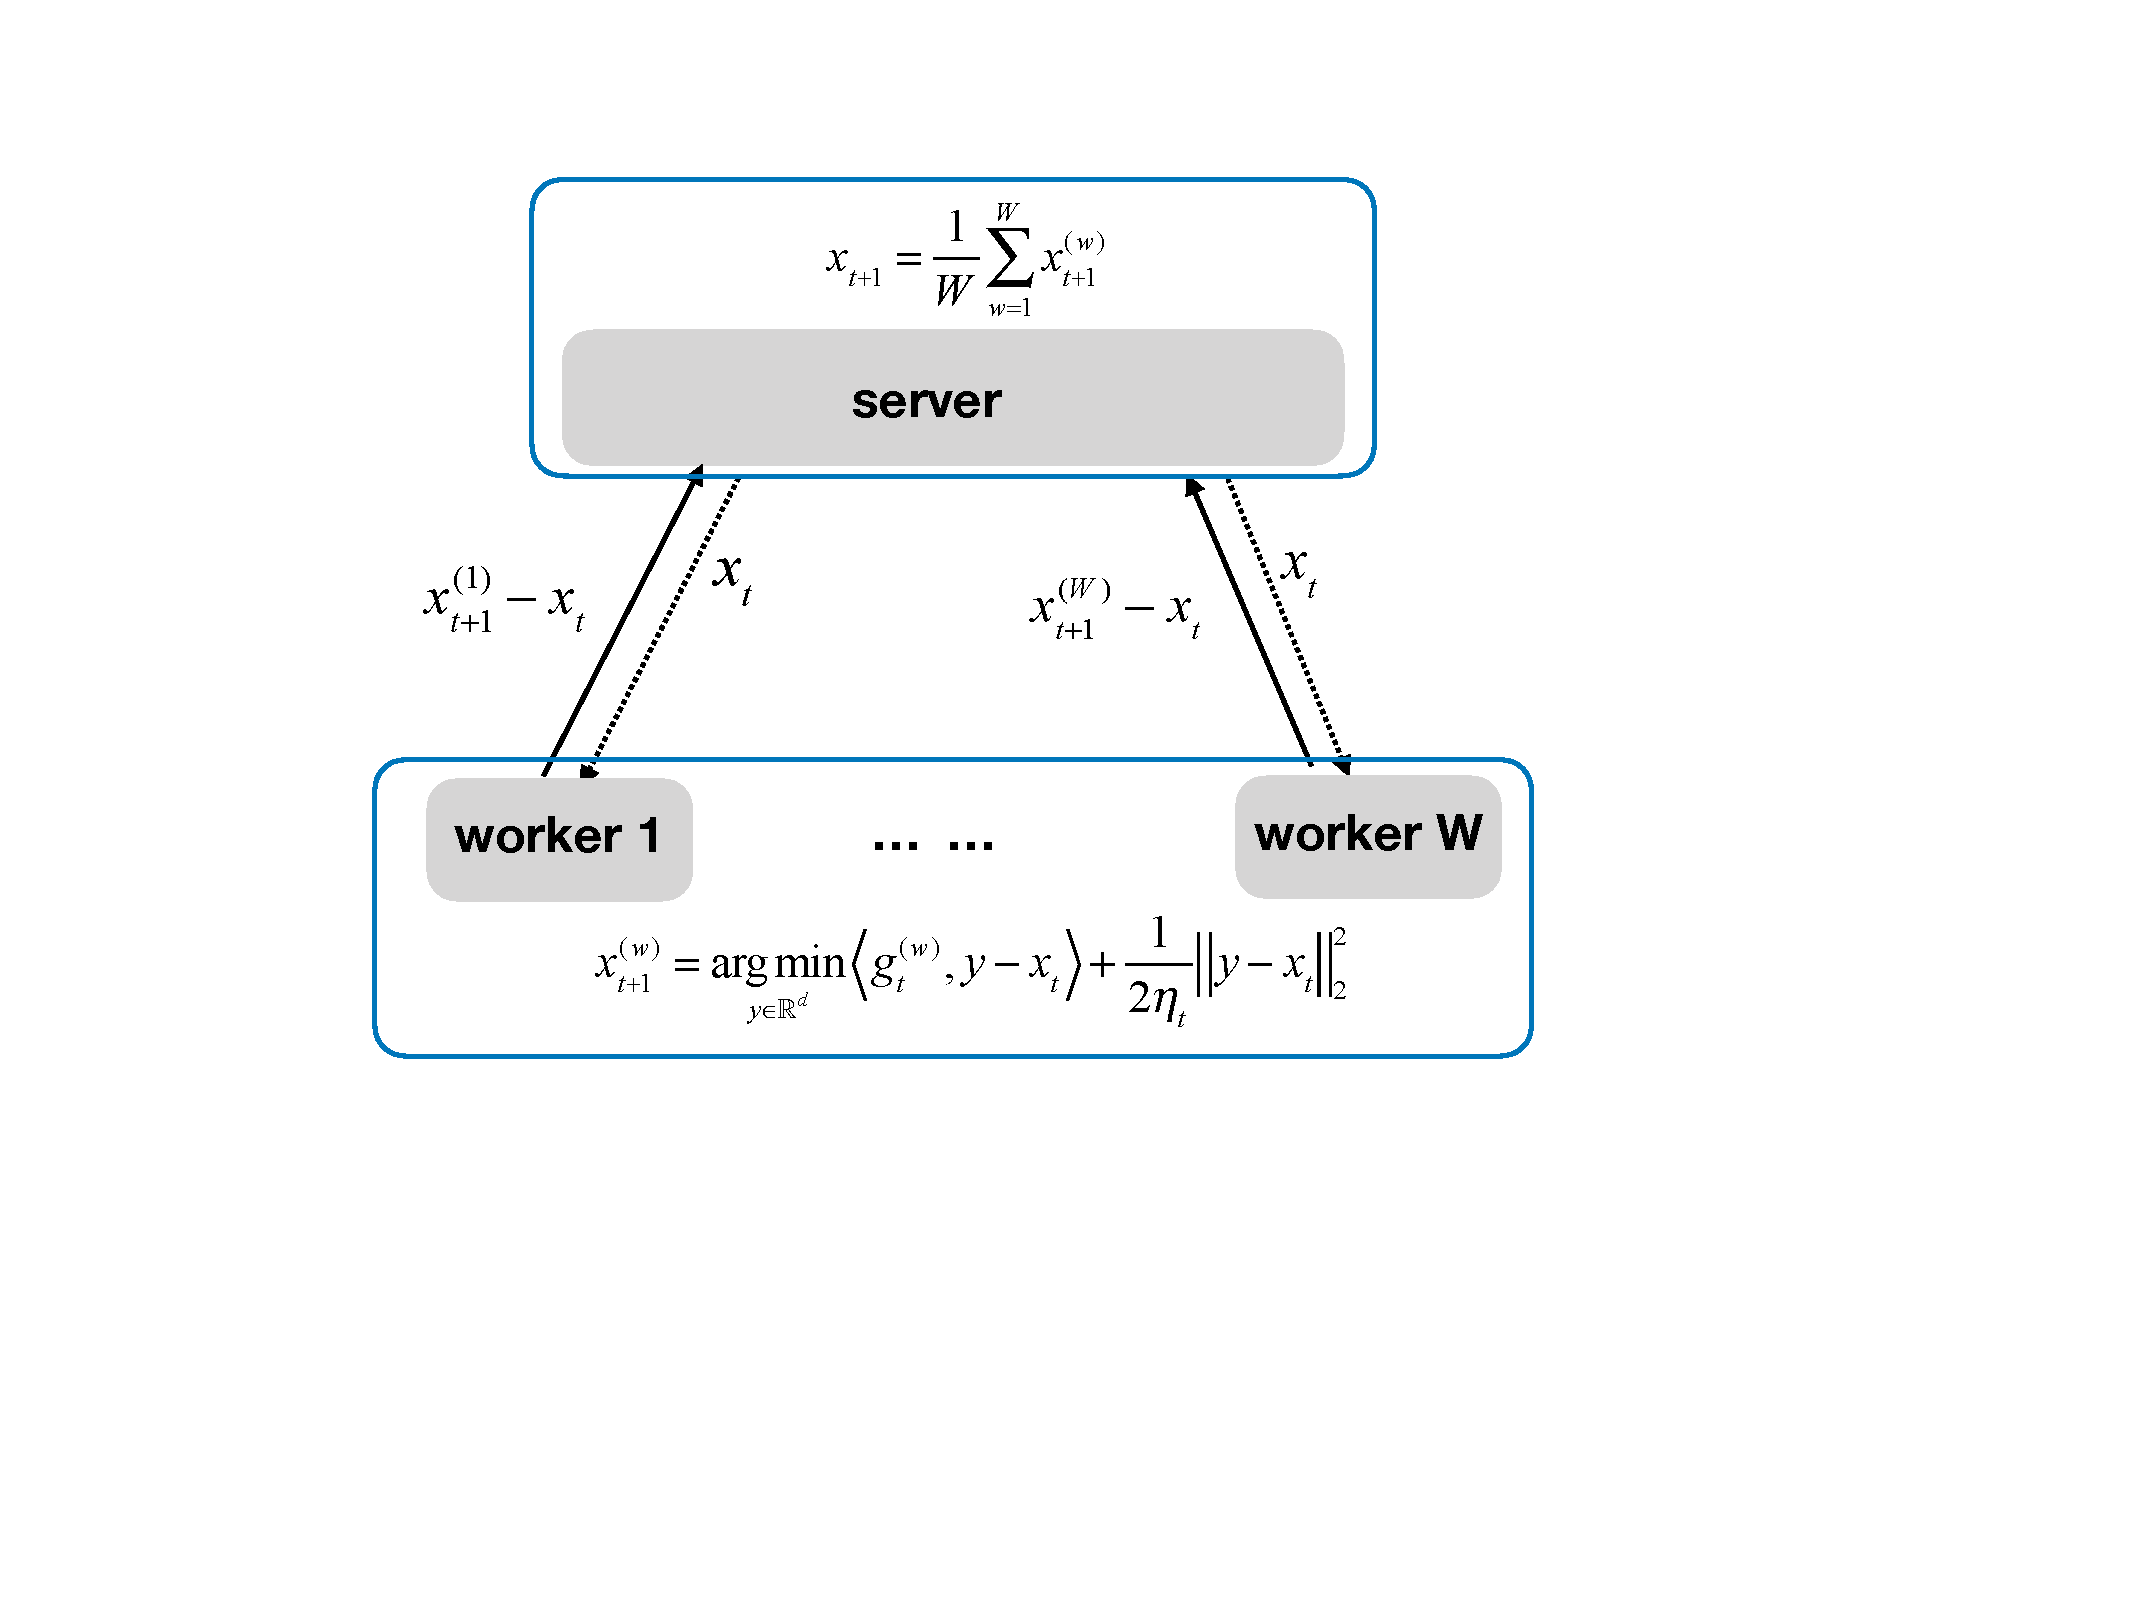
\includegraphics[width=0.7\columnwidth]{figures/figure_preliminary_parameter_server}
\caption{The illustration of the $t+1$-th iteration of the gradient descent method, which is performed  in a parameter server system.}
\label{figure_preliminary_parameter_server}
\end{figure}

\begin{figure}[!t]
\setlength{\abovecaptionskip}{0pt}
\setlength{\belowcaptionskip}{0pt}
\centering 
\subfigure[$\x^{(w)}_{t+1}-\x_t$  without clustering structures]{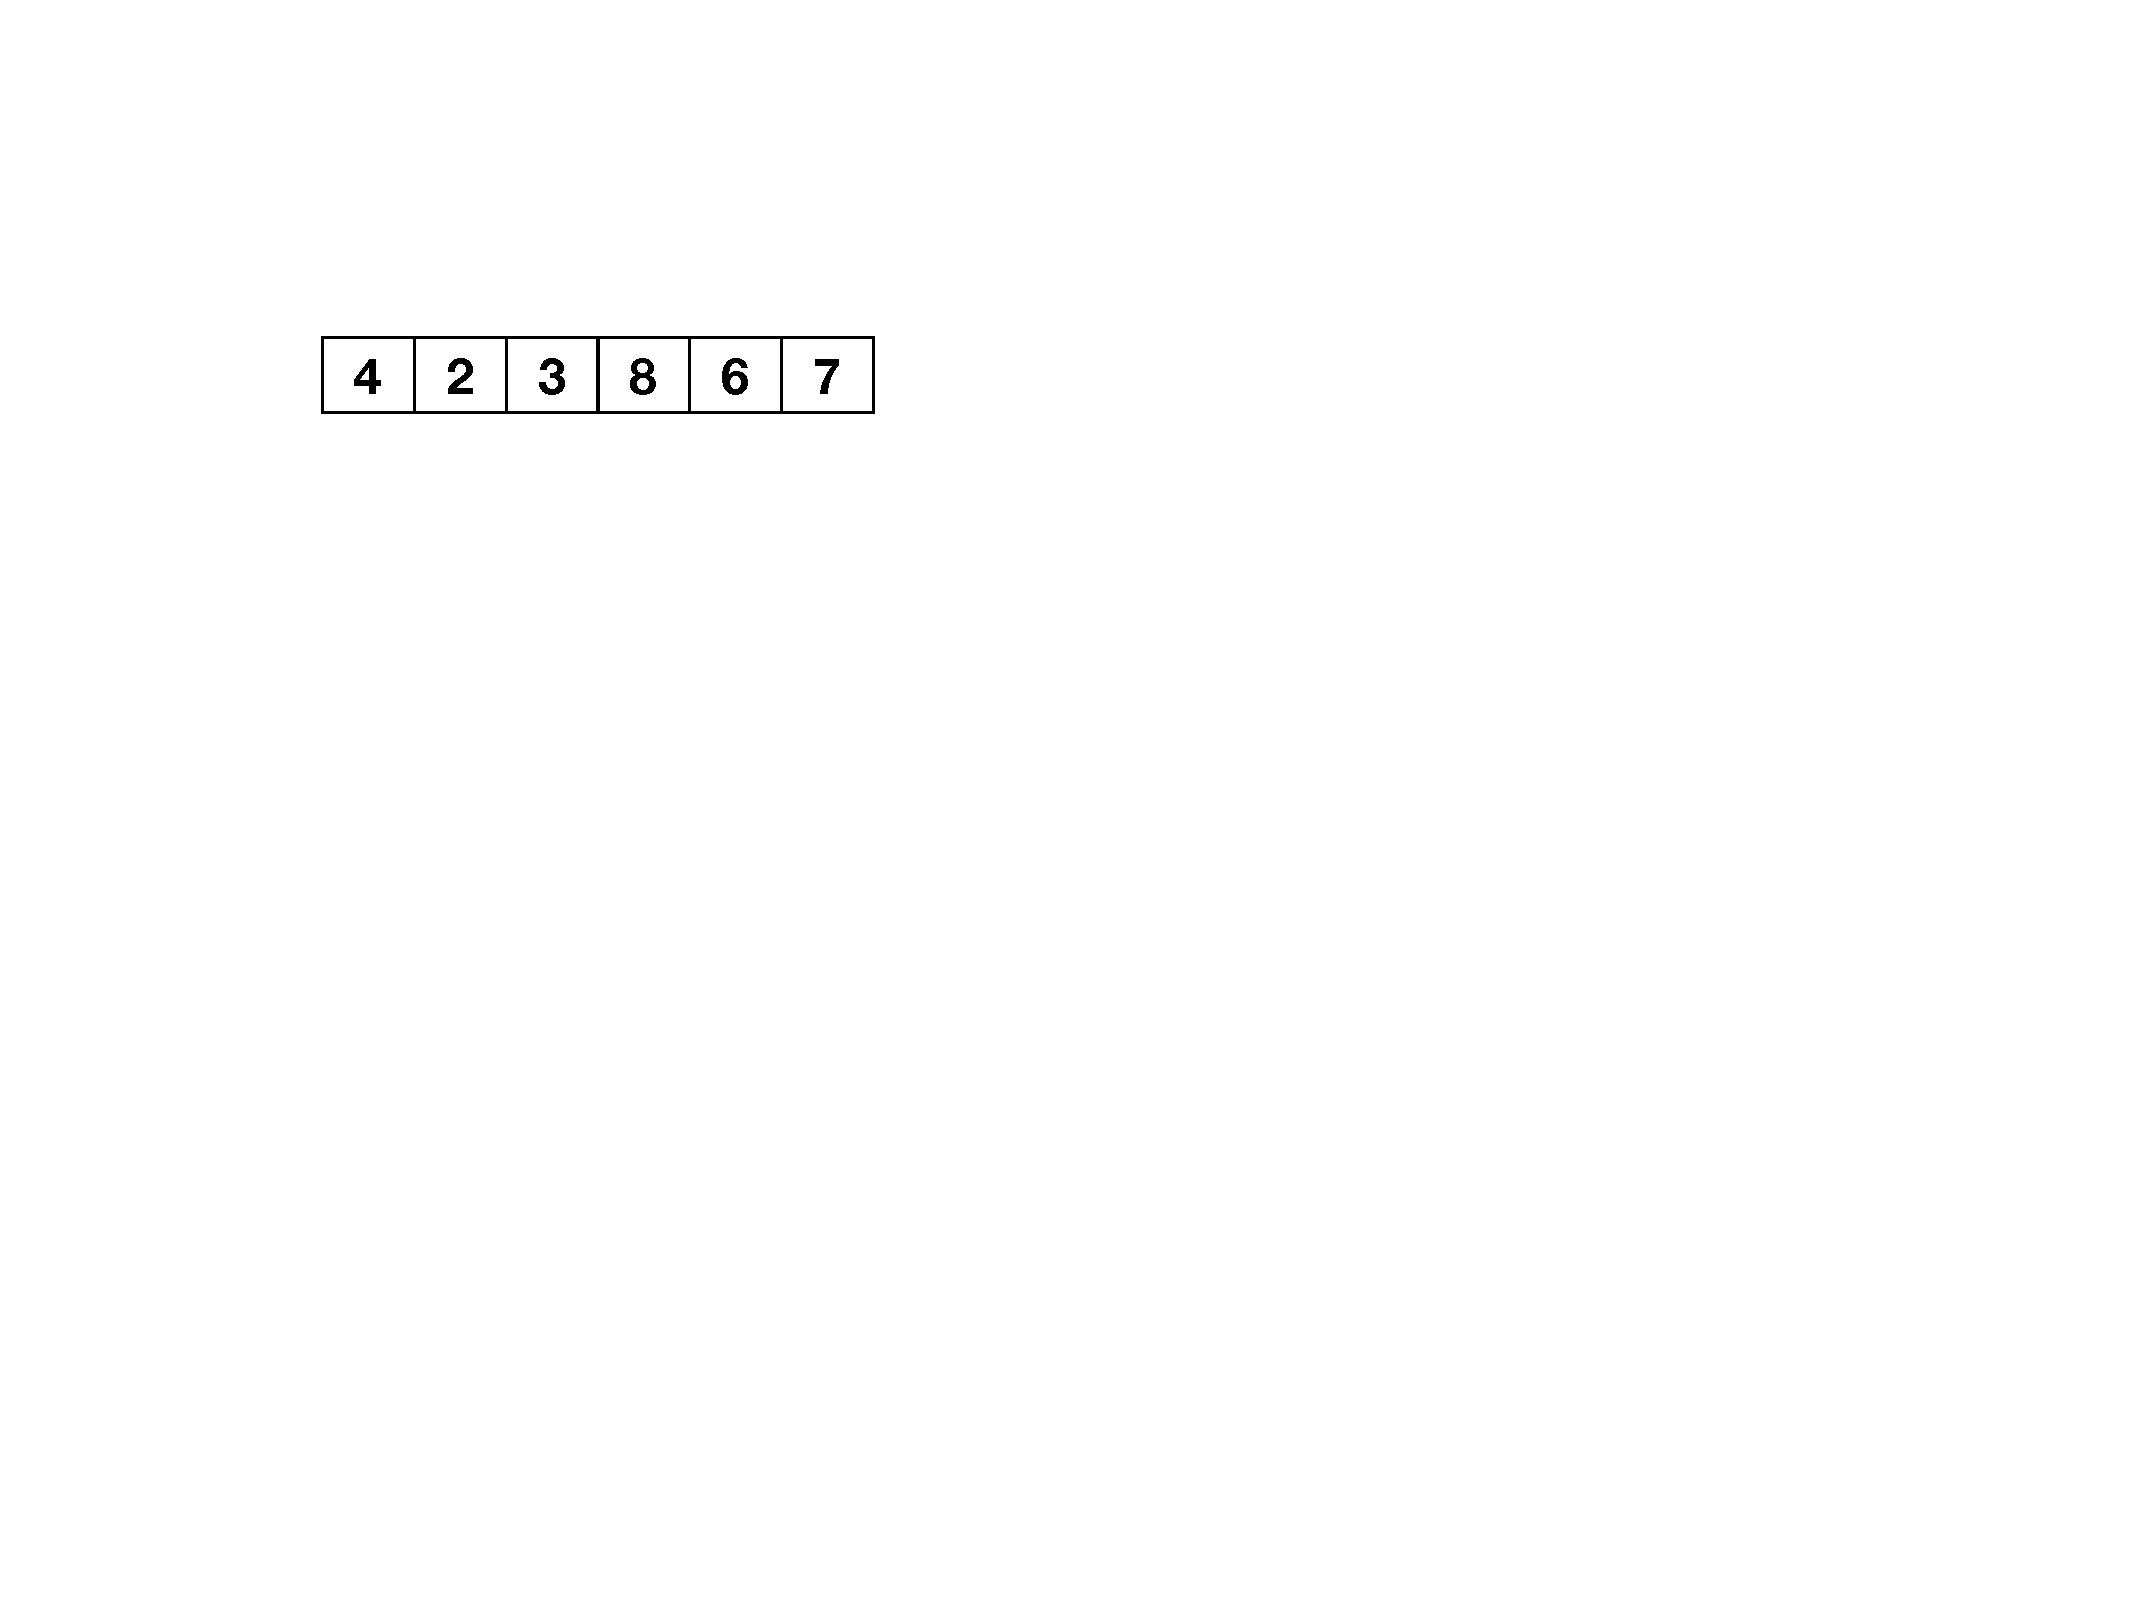
\includegraphics[width=0.4\columnwidth]{figures/figure_intro_gradient_clustering_without_clustering}\label{figure_intro_gradient_clustering_without_clustering}}
\subfigure[Difference between elements of $\x^{(w)}_{t+1}-\x_t$  (without clustering structures) is dense.]{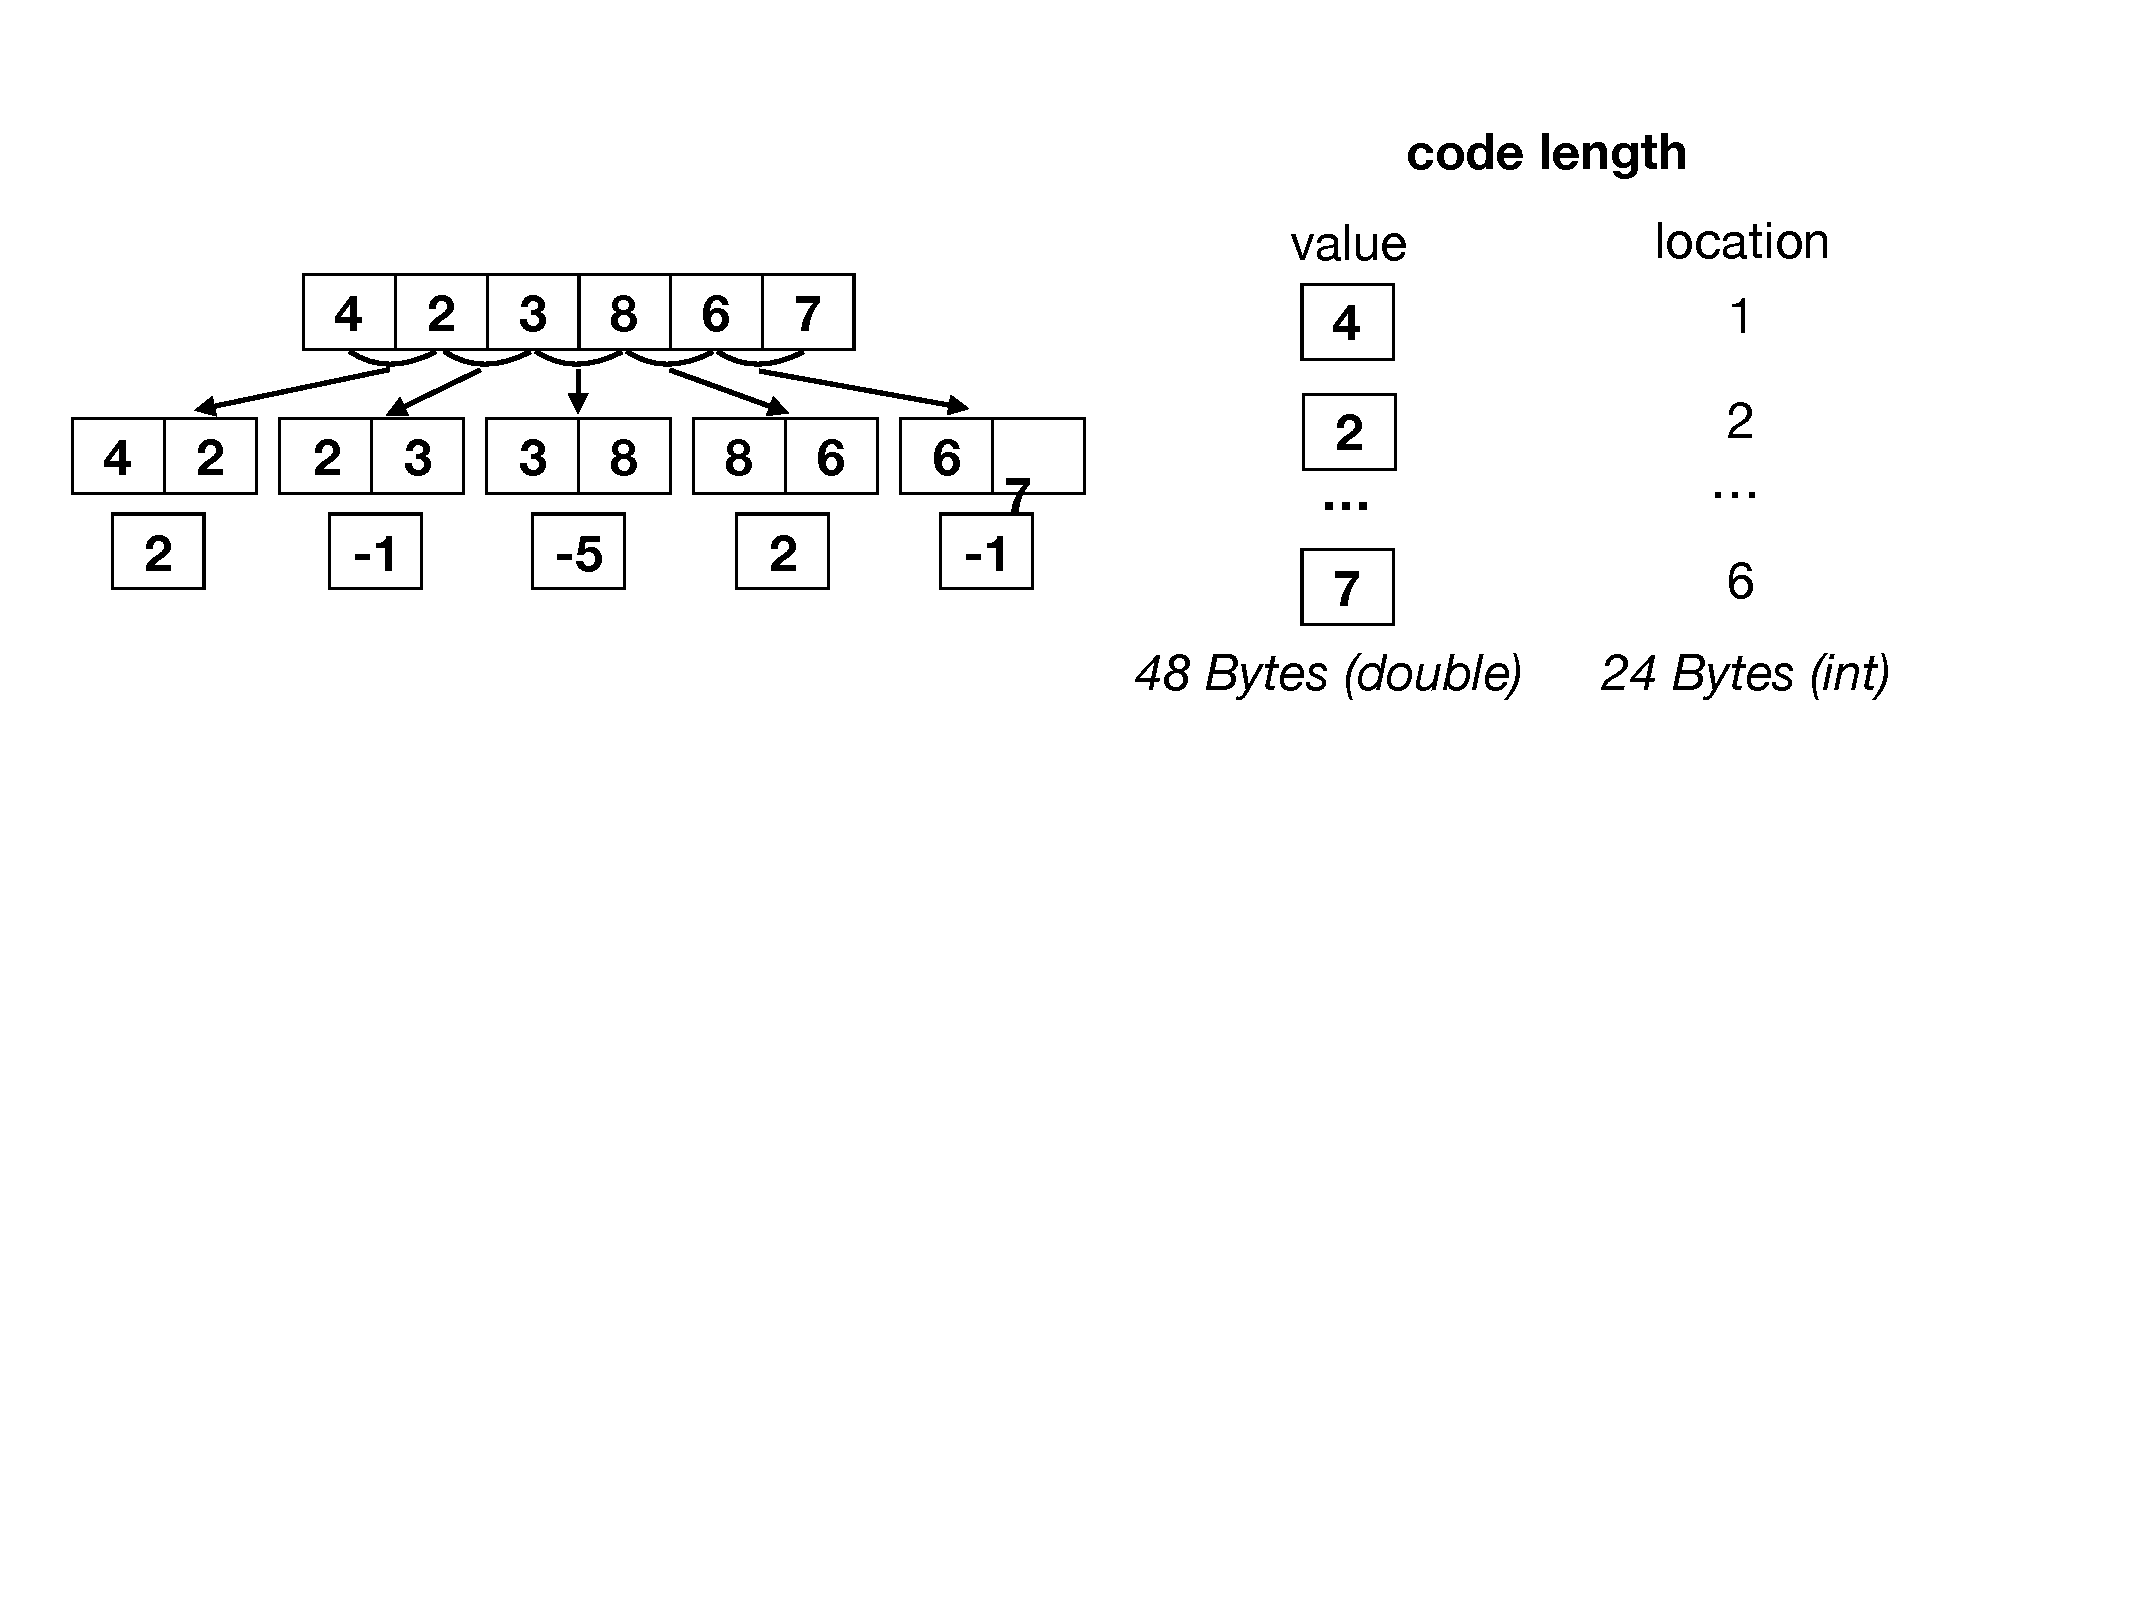
\includegraphics[width=0.8\columnwidth]{figures/figure_intro_gradient_clustering_without_clustering_details}\label{figure_intro_gradient_clustering_without_clustering_details}}
\subfigure[$\x^{(w)}_{t+1}-\x_t$ with clustering structures]{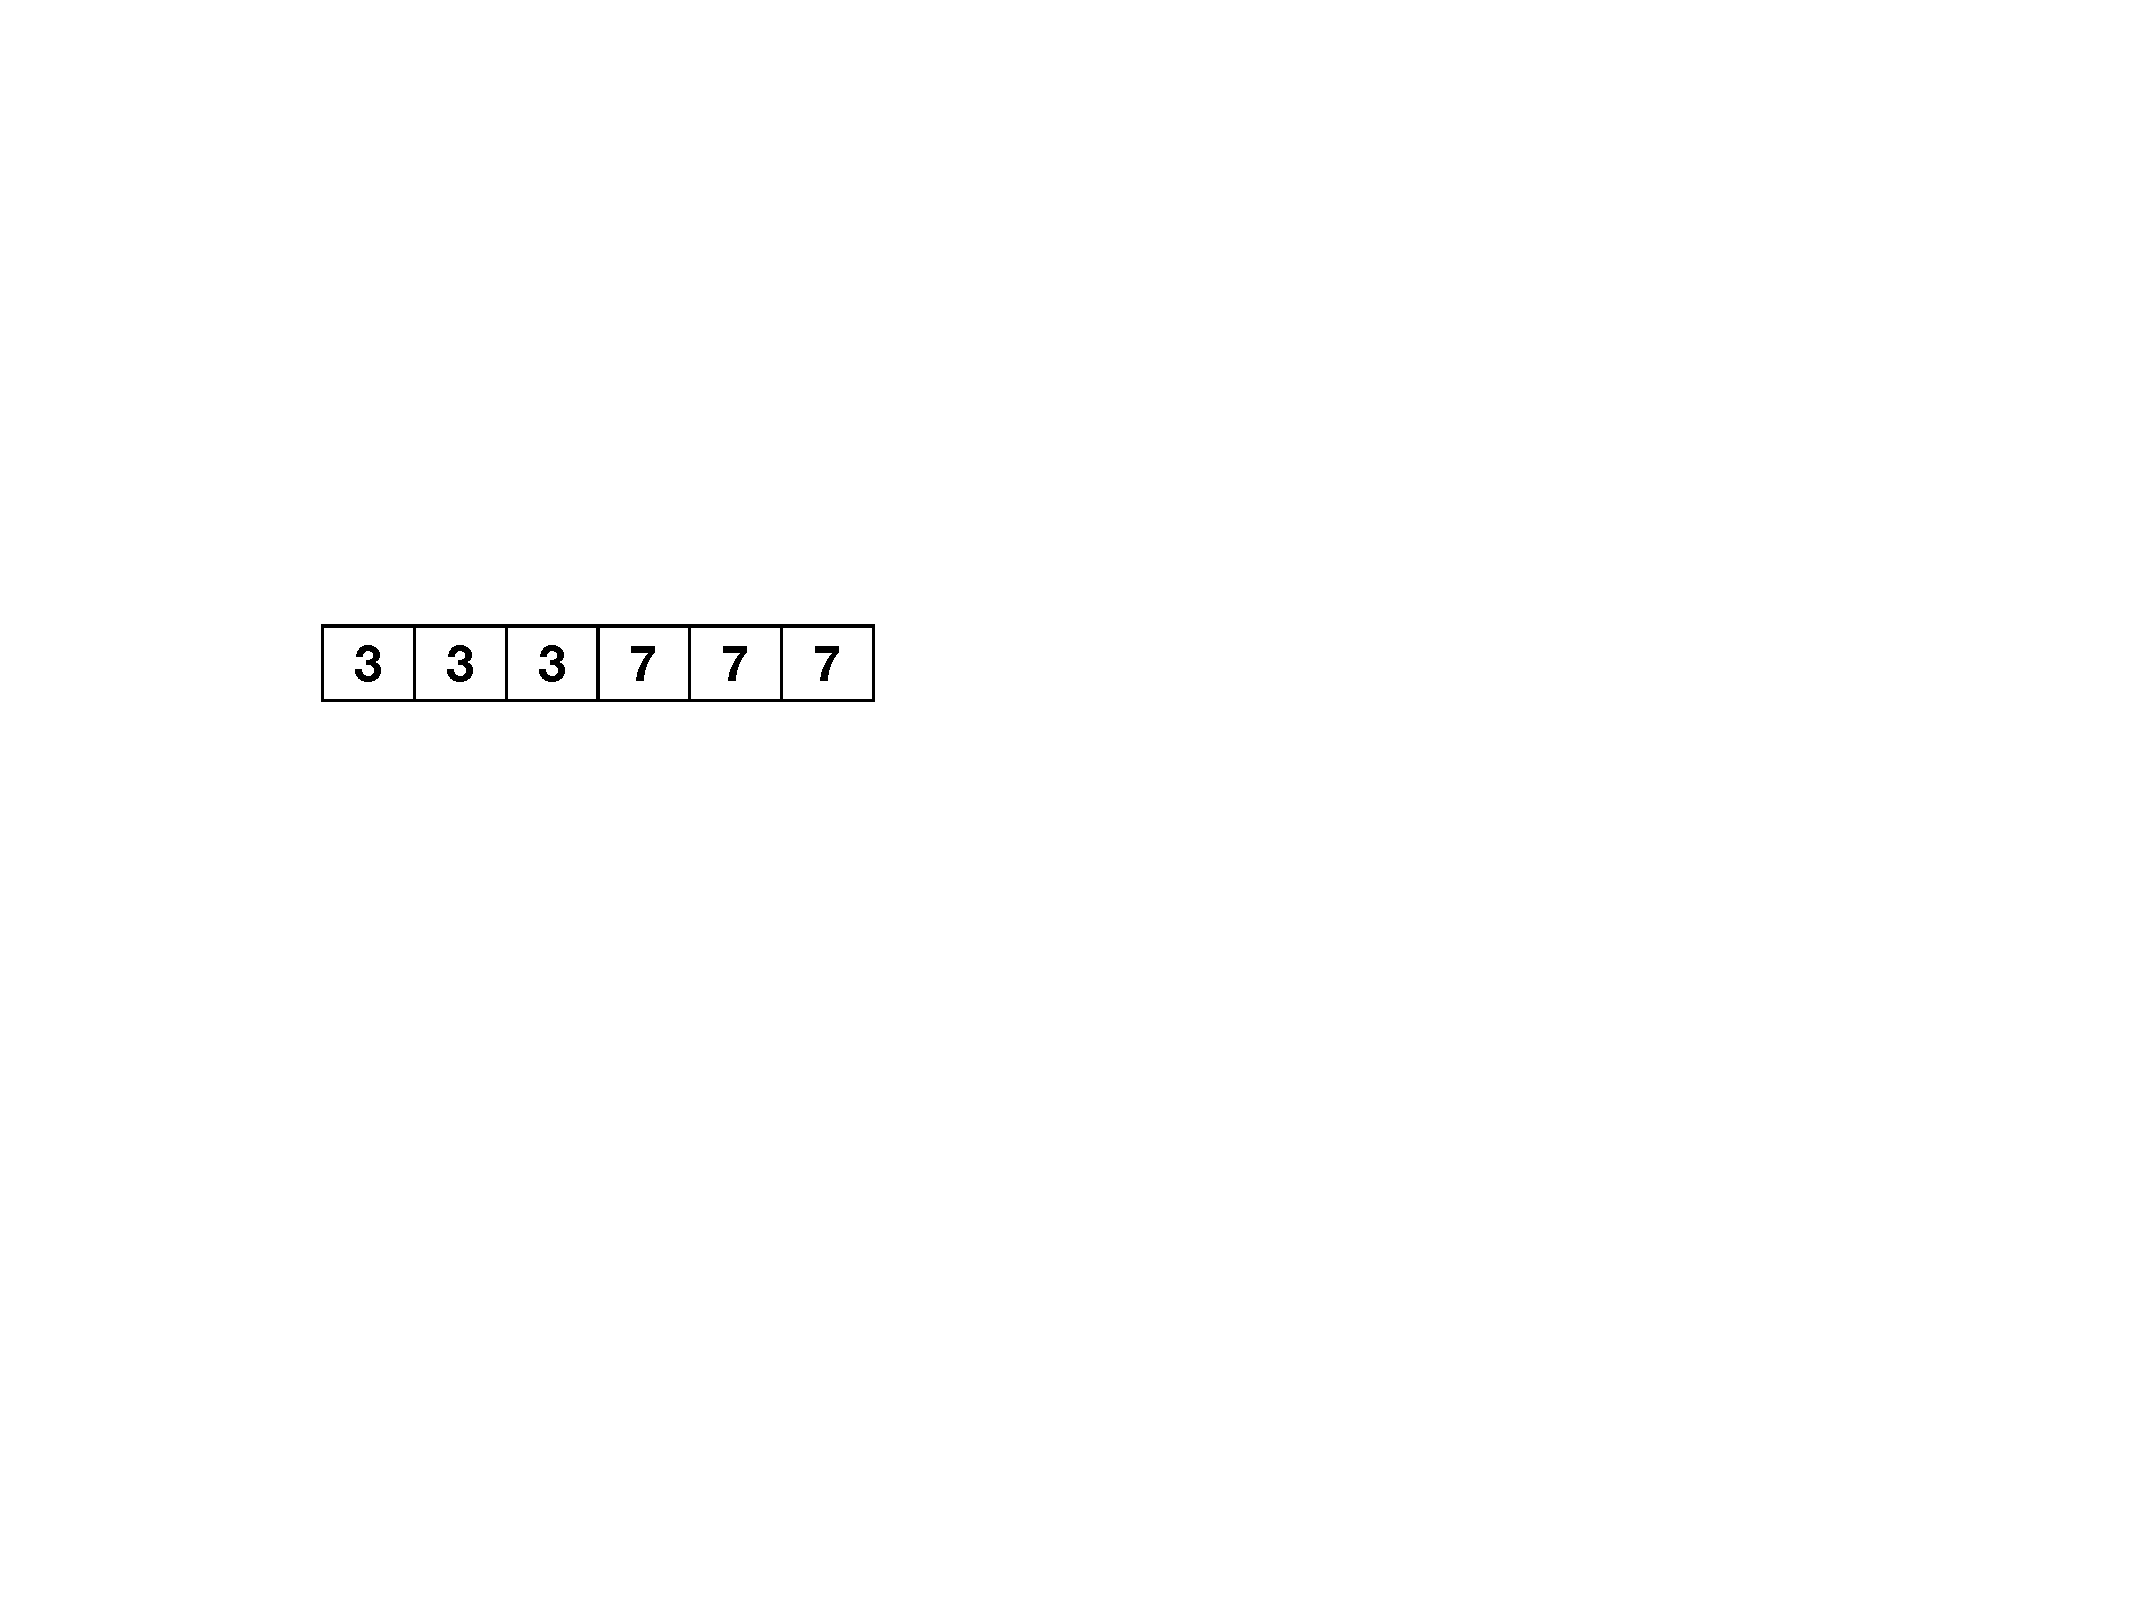
\includegraphics[width=0.4\columnwidth]{figures/figure_intro_gradient_clustering_with_clustering}\label{figure_intro_gradient_clustering_with_clustering}}
\subfigure[Difference between elements of $\x^{(w)}_{t+1}-\x_t$  (with clustering structures) is \textbf{sparse}.]{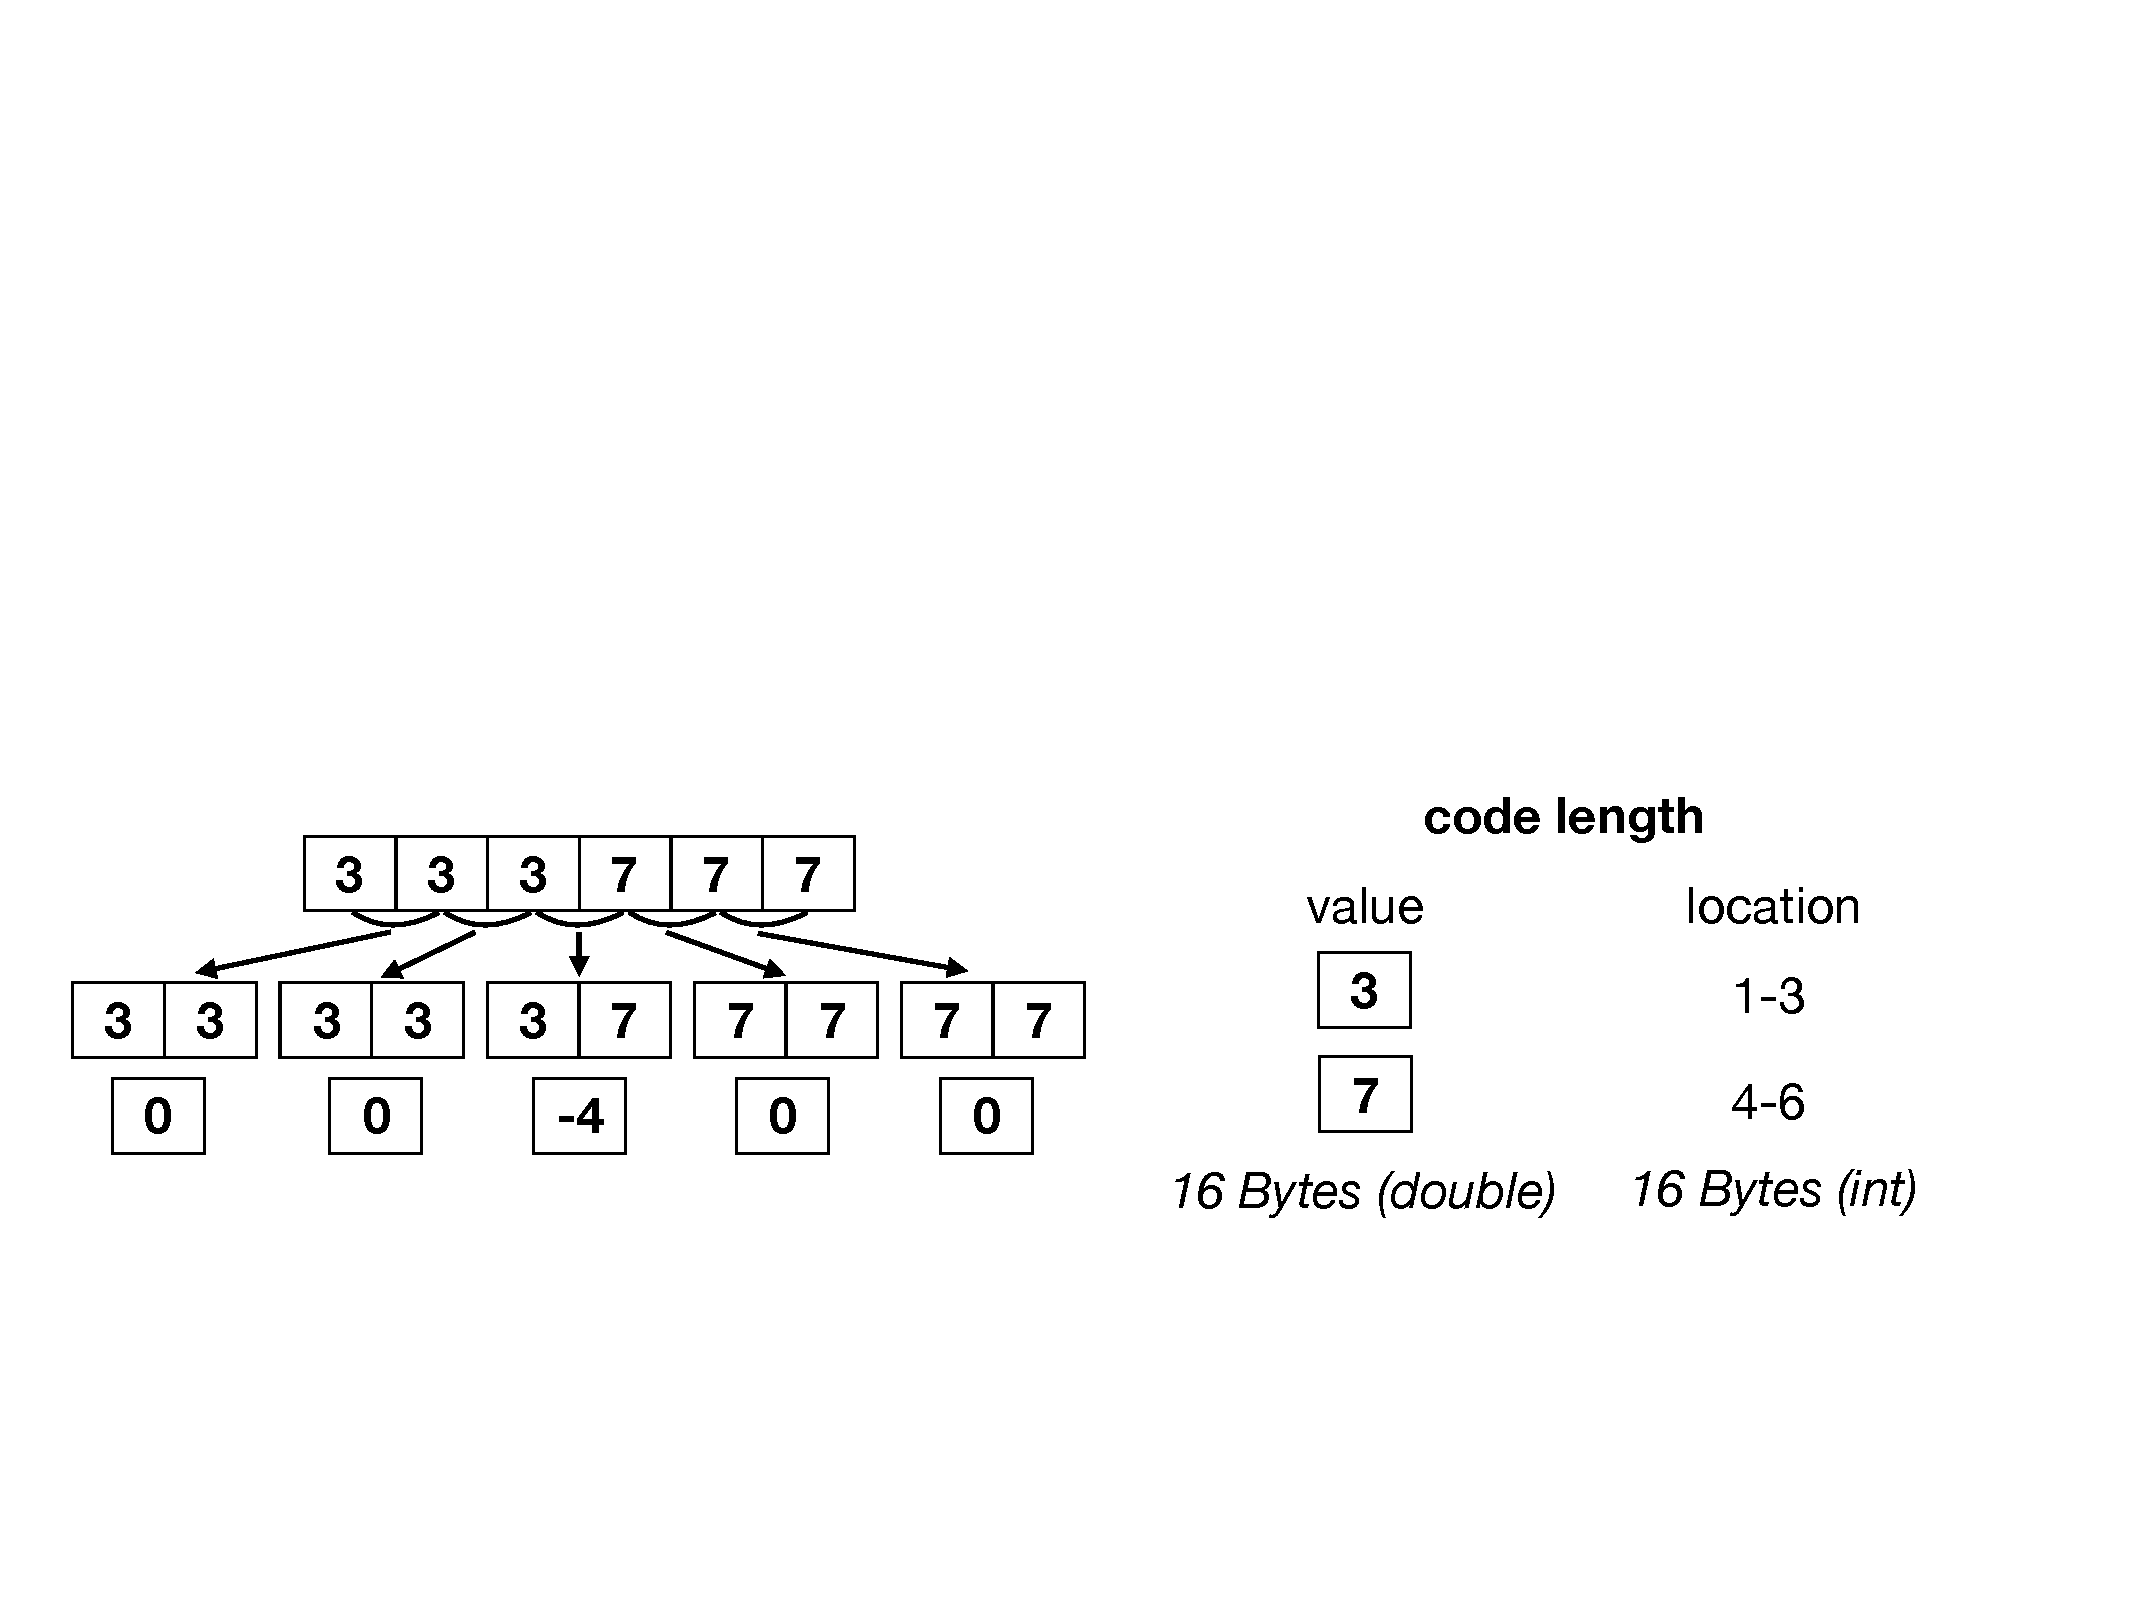
\includegraphics[width=0.8\columnwidth]{figures/figure_intro_gradient_clustering_with_clustering_details}\label{figure_intro_gradient_clustering_with_clustering_details}}
\caption{The illustrative example shows that $\x^{(w)}_{t+1}-\x_t$ with clustering structures can be compressed by using fewer bits, and thus the code length is reduced effectively. \textbf{Our basic idea is to make the difference between  elements of $\x^{(w)}_{t+1}-\x_t$ sparse.}}
\label{figure_intro_gradient_clustering}
\end{figure}

In the paper, we jointly optimize Eq. \eqref{equa_main_optimization_objective} in the distributed setting by using a communication efficient regularizer.  We propose a distributed optimization method, which encourages the update of parameter $\x^{(w)}_{t+1}-\x_t$ to own clustering structures. Figure \ref{figure_intro_gradient_clustering} presents an illustrative example. According to Figures \ref{figure_intro_gradient_clustering_without_clustering} and \ref{figure_intro_gradient_clustering_with_clustering},  we observe when the elements of $\x^{(w)}_{t+1}-\x_t$ own clustering structures, they can be encoded by using fewer bits. Its code length can be reduced a lot. The update of parameter can be transmitted from workers  and the server efficiently. According to Figures \ref{figure_intro_gradient_clustering_without_clustering_details} and \ref{figure_intro_gradient_clustering_with_clustering_details}, our basic idea is to let the difference between the elements of $\x^{(w)}_{t+1}-\x_t$ be sparse, which encourages the elements of $\x^{(w)}_{t+1}-\x_t$ to have clustering structures.

Comparing with the gradient quantization methods in the previous studies, the proposed method is able to find a good tradeoff between the convergence performance and the communication efficiency.  It is highlighted that the proposed method does not impair the convergence performance theoretically. Additionally, we propose an Alternating Direction of Method of Multipliers (ADMM) method to solve Eq. \eqref{equa_main_optimization_objective} efficiently. Furthermore, we improve the proposed method with some useful coding strategies. Finally, extensive empirical studies verify the advantages of the proposed method.  In summary, our main contributions are outlined as follows.
\begin{itemize}
\item We propose a communication efficient regularizer to jointly optimize a machine learning model and the communication efficiency.
\item We propose a new ADMM method to update the parameter efficiently.
\item We prove that the proposed distributed optimization method converges with a sublinear rate theoretically.
\end{itemize}





The paper is organized as follows. Section \ref{sect_related_work} outlines the related work. Section \ref{sect_communication_efficient_optimization}  presents the proposed distributed optimization method by using a communication efficient regularizer. Section \ref{sect_efficient_method_update_parameter} presents the efficient method to conduct the update of parameters. Section \ref{sect_convergence_rate} presents the convergence rate of the proposed method. Section \ref{sect_coding_strategy} presents some useful coding strategies to improve the communication efficiency. Section \ref{sect_experiment} presents extensive empirical studies. Section \ref{sect_conclusion} concludes the paper.

 

\section{Related work}
\label{sect_related_work}
We review the previous related literatures briefly.

\subsection{Methods to reduce the number of rounds of communication}
 \cite{Zhang:2013wq,pmlr-v65-wang17a,Smith:2016wp,Jaggi:2014,Shamir:2014:CDO,pmlr-v37-zhangb15,Reddi:2016wm} develop flexible methods to reduce the number of rounds of communication for the distributed optimization. For example, \cite{Zhang:2013wq} proposes a new sub-sampling method to reduce the number of rounds of communication.  \cite{pmlr-v65-wang17a} proposes a method to reduce the required memory for communication and the number of rounds of communication. Additionally, \cite{Renggli:2018uf} designs a communication-efficient protocol to reduce the workload of communication when handling the sparse dataset. \cite{Ye:2018uc} develops a new coding method for gradients to make a good trade-off between the computation and communication, but there is no theoretical guarantee for the convergence rate. Comparing with the proposed method, those previous researches do not involve in the compression of the update of parameter, and are orthogonal to our work. Therefore, these researches can be used to improve our method. 

\subsection{Methods to reduce the code length of gradients}
\cite{Xie:2016vt} proposes a sufficient factor broadcasting method to reduce the workload of network communication in a parameter server system. Since it is designed for matrix-parametrized models, it is not suitable for a general machine learning model such as ridge regression. \cite{alhamaji2017} improves the communication efficiency by making the gradient sparse with no theoretical guarantee. \cite{NIPS2017_6768,Zhang:2016wx} propose gradient quantization methods to reduce the code length of gradients. \cite{Wangni:2017vj} makes the gradient sparse to reduce its code length.  Comparing with the proposed method, those previous researches separately consider the learning of a machine learning model and the improvement of the communication efficiency. The proposed method outperforms them by making a good tradeoff between the convergence and the communication efficiency, which does not impair the convergence rate theoretically. 


\section{ Distributed optimization with the communication efficient regularizer }
\label{sect_communication_efficient_optimization}
In the section, we first show the major notations, and propose the  communication efficient regularizer.  Then, we present our distributed optimization method.

\subsection{Notations}
\begin{itemize}
{\color{blue} 
\item The regular letters $W$ and $w$ represent scalars. $W$ represents the number of workers in a parameter server system, and $w\in[W]$ means the $w$-th worker.
\item The bold lower-case letter $\x$ represents the parameter of a machine learning problem, and its $i$-th element is represented by $\x^i$. 
\item The bold upper-case letter $\A$ represents the data matrix, and the $i$-th row of $\A$ represents the $i$-th instance. 
}
\item The bold upper-case letter $\Q$ represents a matrix, and its $i$-th row is represented by $\Q^i$.
\item $\g_t^{(w)}$ represents the stochastic gradient at the $t$-th iteration for the $w$-th worker. $M$ and $d$ represent the number of instances in the dataset and the dimension of every instance, respectively. 
\item $\sigma$ represents the smallest singular value of $\Q$. 
\item $\lrnorm{\cdot}_s$  represents the $\ell_s$-norm with $s \in \{1,2,\infty\}$.
\item $B_p(\z,\x)$ represents the $p$-norm Bregman divergence, which is defined by $B_p(\z,\x) := \phi(\z) - \phi(\x) - \lrangle{\nabla \phi(\x), \z-\x}$ with $\phi(\x) := \frac{1}{2}\lrnorm{\x}_p^2$. Here, $1<p\le 2$.
{\color{blue} 
\item For any $\a$ and $\b$, $\lrangle{\a,\b}$ means $\a\Tr\b$, that is the inner product of $\a$ and $\b$.
}
\item $\EE$ represents to take mathematical expectation, and $\nabla $ represents the gradient operator. 
\item $\text{sign}(a) = 1$ if $a>0$, $\text{sign}(a) = -1$ if $a<0$, and $\text{sign}(a) = 0$ if $a=0$.
\end{itemize}

  


\subsection{CER: communication Efficient Regularizer}
{\color{blue}
Recall that stochastic gradient descent is usually used to solve a general optimization problem Eq. \eqref{equa_main_optimization_objective}. The Distributed Stochastic Gradient Descent (DSGD) method is performed iteratively. The previous DSGD conducts the update of parameter by solving Eq. \eqref{equa_sgd_local_update}. Since every worker has to send the update of parameter $\x^{(w)}_{t+1}-\x_t$ to the server, the workload of the network communication  becomes very  heavy for a large number of workers. When the workload of the the network communication is heavy, the previous DSGD has to consume much time to complete the data transmission, which impairs the convergence performance of DSGD.  

To improve the communication efficiency of DSGD, we propose a new method to conduct the update of the parameter, instead of solving Eq. \eqref{equa_sgd_local_update} directly. The proposed method use a communication efficient regularizer to find clustering structures of the elements of $\x^{(w)}_{t+1}-\x_t$. It is formulated as
\begin{align}
\label{equa_update_rule_cer}
\x^{(w)}_{t+1} = \argmin_{\y\in\RR^d} \quad \lrangle {\g^{(w)}_t, \y - \x_{t} } + {1\over 2\eta_t} \lrnorm{\Q(\y - \x_t)}_1^2.
\end{align} 
}Here, $\g^{(w)}_t$ is a stochastic gradient, which is obtained by using the local data in the $w$-th worker. The given full rank square matrix $\Q\in\mathbb{R}^{d\times d}$ is defined by
\begin{align}
\nonumber
\Q := \begin{bmatrix}
 1&  -1&  &  & \\ 
 &  1&  -1&  & \\ 
 &  &   \cdots &  & \\ 
 &  &  & 1 & -1 \\ 
 &  &  &  & 1
\end{bmatrix}.
\end{align} Notice that $\Q$ is a full rank square matrix, whose smallest singular value, denoted by $\sigma$,  is positive, that is, $\sigma > 0$. Comparing with the previous updating rule, i.e., Eq. \eqref{equa_sgd_local_update}, the proposed communication efficient regularizer is an $\ell_1$ norm square. It punishes the difference between elements of $\x^{(w)}_{t+1}-\x_t$, and encourages them  to be small or even zero. Thus, those corresponding elements of $\x^{(w)}_{t+1}-\x_t$ are very similar or even identical. That is, the elements of $\x^{(w)}_{t+1}-\x_t$ own clustering structures. Exploiting the clustering structures, $\x_{t+1}$ can be compressed by using few bits, and thus improves the communication efficiency in the distributed setting.

We give a demo example to explain the communication efficient regularizer intuitively. Suppose the optimum of $\x\in\RR^4$ is $\x_{\ast} = (1, -1, 1, -1)\Tr$. If $\x_0 = (0,0,0,0)\Tr$, the communication efficient regularizer may update $\x$ as follows.
\begin{align}
\nonumber
\x_1 = & (-1,-1,1,1)\Tr, \text{ and } \Q(\x_1-\x_0)= (0,-2,0,1)\Tr \\ \nonumber
\x_2 = & (1,-1,1,1)\Tr, \text{ and } \Q(\x_2-\x_1) = (2,0,0,0)\Tr \\ \nonumber
\x_3 = & (1,-1,1,-1)\Tr, \text{ and } \Q(\x_3-\x_2) = (0,0,2,-2)\Tr.
\end{align} For $\x_1$, $\x_2$ and $\x_3$, there are only two different elements: `$1$' and `$-1$', which shows that there are two clusters among those elements, and their cluster centers are `$1$' and `$-1$', respectively. Meanwhile, the difference of elements between successive update, e.g., $\Q(\x_2-\x_1)$, containts as least two $0$s. \textbf{It explains our basic idea, that is, to let the difference between elements of successive update, i.e., $\Q(\x^{(w)}_{t+1}-\x_t)$, be sparse.} 
 
However, comparing with Eq. \eqref{equa_sgd_local_update}, it is challenging for Eq. \eqref{equa_update_rule_cer} to obtain sublinear convergence rate in theoretical. The reason is that the communication efficient regularizer is non-smooth. Intuitively, it makes a tradeoff between the convergence performance and the communication efficiency. To improve the communication efficiency, the convergence performance may be impaired. This challenging problem is solved in the following section.

\subsection{Communication efficient update  with a linear coupling strategy}
 
\begin{algorithm}[!t]
    \caption{Distributed optimization with the communication efficient regularizer}
    \label{algo_comm_effi_regu_master}
    \begin{algorithmic}[1]
        \Require The number of total iterations $T$, and the initial parameter $\x_1$.
        \algotext{\textbf{On the server:}}
        \For {$t=1,2, ..., T$}
            \State Deliver the parameter $\x_t$ to every worker.
            \State Wait to collect all updates of  parameter $\y_{t+1}^{(w)} - \x_t$ with $1\le w \le W$.
            \State Update the global parameter $\x_{t+1} = \frac{1}{W}\sum\limits_{n=1}^W\y_{t+1}^{(w)}$.
        \EndFor
        \Return $\x_{T+1}$.
        \algotext{\textbf{On the $w$-th worker for the $t+1$-th iteration:}}
        \State Receive the parameter $\x_t$ from the server.
        \State $\eta_t = \frac{\sigma^2}{2L_1 \sqrt{t}}d^{-1}$, and $\x_{t+1}^{(w)} = \frac{1}{2}(\z_t^{(w)} + \x_t)$.
        \State Randomly sample an instance $\a$, and compute the stochastic gradient $\g^{(w)}_t = \nabla f(\x_{t+1}^{(w)};\a)$.
        \State $\y_{t+1}^{(w)} = \argmin_{\y\in\RR^d} \lrangle{\g^{(w)}_t, \y - \x_t} + \frac{1}{2\eta_t}\lrnorm{\Q(\y- \x_t)}_1^2$.
        \State $\z_{t+1}^{(w)} = \argmin_{\z\in\RR^d} \lrangle{\g^{(w)}_t, \z - \x_{t+1}^{(w)}} + \frac{1}{2\alpha_t}B_p(\z, \x_{t+1}^{(w)})$, and $B_p(\z, \x_{t+1}^{(w)}) = \frac{1}{2}\lrnorm{\z - \x_{t+1}^{(w)}}_p^2$.
        \State Send $\y_{t+1}^{(w)} - \x_t$ to the server.
    \end{algorithmic}
\end{algorithm} 


Consider Eq. \eqref{equa_update_rule_cer} on the $w$-th worker in the distributed setting. We do not transmit the sequence of $\{\x_{t+1}^{(w)}\}_{t=1}^T$ directly. Instead, we maintain two sequences $\{\y^{(w)}_t\}_{t=1}^T$ and $\{\z^{(w)}_t\}_{t=1}^T$ on the $w$-th worker, and a sequence $\{\x_t\}_{t=1}^T$ on the server. Every $\x_{t+1}$ is defined by 
\begin{align}
\nonumber
\x_{t+1} = \frac{1}{W}\sum_{w=1}^W \y_{t+1}^{(w)}.
\end{align}  We then use a linear coupling strategy $\x_{t+1}^{(w)} = \frac{1}{2} \lrincir{\z_t^{(w)} + \y_t} $ to guarantee the sublinear convergence rate. 

$\y_{t+1}^{(w)}$ is yielded based on $\x_{t+1}^{(w)}$ by using Eq. \eqref{equa_update_rule_cer}, that is,
\begin{align}
\label{equa_update_rule_cer_distributed}
\y_{t+1}^{(w)} = \argmin_{\y\in\RR^d} \quad \lrangle{ \g_t^{(w)}, \y - \x_{t+1}^{(w)} } + {1\over 2\eta_t} \lrnorm{\Q(\y - \x_{t+1}^{(w)})}_1^2.
\end{align} Here, $\eta_t$ is a learning rate, which is usually set to be positively proportional to $\frac{1}{\sqrt{t}}$. $\y_{t+1}^{(w)} - \x_t$  is transmitted to the server, and shared with other workers. Benefiting from the intrinsic clustering structures in elements of $\y_{t+1}^{(w)} - \x_t$,  it can be transmitted in a communication efficient way. Additionally, we maintain a local sequence of $\{ \z_t^{(w)} \}_{t=1}^T$, which is obtained by 
\begin{align}
\label{equa_update_rule_cer_distributed_z}
\z_{t+1}^{(w)} = \argmin_{\z\in\RR^d} \lrangle{\g^{(w)}_t, \z - \x_{t+1}^{(w)}} + \frac{1}{2\alpha_t}B_p(\z, \x_{t+1}^{(w)}).
\end{align} Here, $B_p(\z, \x_{t+1}^{(w)}) := \phi(\z) - \phi(\x_{t+1}^{(w)}) - \lrangle{\nabla \phi(\x_{t+1}^{(w)}), \z - \x_{t+1}^{(w)}}$. $\phi(\x) := \frac{1}{2}\lrnorm{\x}_p^2$ and $1<p\le 2$ is the $p$-norm Bregman divergence \cite{Duchi:2010tk}.  Note that $\z_{t+1}^{(w)}$ is stored in the local worker, and is not shared with other workers. 


{\color{blue}
The introduction of $\z_{t+1}^{(w)}$ and $\z_{t+1}^{(w)}$
\begin{itemize}
\item The sequence $\{\y_t^{(w)}\}_{t=1}^T$ is shared with other workers. Since the elements of  every $\y_t^{(w)}$ own clustering structures, it can be transmitted efficiently. 
\item The sequence $\{\z_t^{(w)}\}_{t=1}^T$ is not shared with other workers. It is used to  help the sequence $\{\y_t\}_{t=1}^T$ converge at the sublinear  rate theoretically.
\end{itemize} 
}The details of our method are presented in Algorithm \ref{algo_comm_effi_regu_master}. 

However, it is challenging to solve Eq. \eqref{equa_update_rule_cer_distributed} (or Eq. \eqref{equa_update_rule_cer}) efficiently. The reason is that the communication efficient regularizer in Eq. \eqref{equa_update_rule_cer_distributed} (or Eq. \eqref{equa_update_rule_cer}) is non-smooth and non-separable. In the next section, we propose an efficient ADMM method to solve Eq. \eqref{equa_update_rule_cer_distributed} (or Eq. \eqref{equa_update_rule_cer}), and present the closed form to solve Eq. \eqref{equa_update_rule_cer_distributed_z}.  







\section{Efficient methods to update {\lowercase{$\y_{t+1}^{(w)}$}} and {\lowercase{$\z_{t+1}^{(w)}$}}}
\label{sect_efficient_method_update_parameter}
In the section, we propose an efficient ADMM method to update $\y_{t+1}^{(w)}$, and then present the closed form to update $\z_{t+1}^{(w)}$.

As we have shown, the communication efficient regularizer makes the update rule, i.e., Eq. \eqref{equa_update_rule_cer_distributed} non-separable and non-smooth. It is challenging to solve it directly. By using the ADMM method, we decompose Eq. \eqref{equa_update_rule_cer_distributed} into some sub-problems, and each of them is able to be solved efficiently. 




\subsection{Update of $\y_{t+1}^{(w)}$.}
Recall that the update of $\y_{t+1}^{(w)}$ is equivalent to be formulated as the following problem.
\begin{align}
\nonumber
\min_{\y\in\RR^d, \u\in\RR^d} \lrangle{\g_t^{(w)}, \y - \x_{t+1}^{(w)}} + \frac{1}{2\eta_t}\lrnorm{\u}_1^2
\end{align} subject to
\begin{align}
\nonumber
\u = \Q(\y- \x_{t+1}^{(w)}).
\end{align} The augmented Lagrangian multiplier is 
\begin{align}
\nonumber
L(\y, \u, \blambda) = \lrangle{\g_t^{(w)}, \y - \x_{t+1}^{(w)}} + \frac{1}{2\eta_t}\lrnorm{\u}_1^2 + \blambda\Tr \lrincir{\Q(\y-\x_{t+1}^{(w)})-\u} + \frac{\rho}{2} \lrnorm{\Q(\y-\x_{t+1}^{(w)})-\u}_2^2,
\end{align} where $\rho$ is the step size.  At the $k$-th iteration, the update of $\y$ is $\hat{\y}_{k+1} = \argmin_{\y\in\RR^d} L(\y, \u_k, \blambda_k)$, which is equivalent to 
\begin{align}
\nonumber
\hat{\y}_{k+1} = &  \argmin_{\y\in\RR^d} \lrangle{\g_t^{(w)}, \y} + \blambda_k\Tr \lrincir{\Q\y-\u_k} + \frac{\rho}{2} \lrnorm{\Q(\y-\x_{t+1}^{(w)})-\u_k}_2^2 \\ \nonumber
= &  \argmin_{\y\in\RR^d} \lrangle{\g_t^{(w)} +  \Q\Tr \blambda_k, \y} + \frac{\rho}{2} \lrnorm{\Q(\y-\x_{t+1}^{(w)})-\u_k}_2^2
\end{align} According to KKT conditions, we obtain
\begin{align}
\nonumber
\hat{\y}_{k+1} = \x_t - \frac{1}{\rho} \lrincir{\Q\Tr\Q}^{-1}\g + \Q^{-1} \lrincir{\u_k - \frac{1}{\rho}\blambda_k}.
\end{align}

\begin{algorithm}[!t]
\caption{ The efficient projected gradient descent method to solve Eq. \eqref{equa_projected_gradient_descent} \cite{Duchi2008Efficient}}    
\label{algo_projected_gradient_descent}
    \begin{algorithmic}[1]
    \Require The positive integer $R$, and positive $\gamma_r$.
    \For {$r=0, 1, ..., R-1$}
        \State $\nabla h(\bdelta_r) = (h_r(\bdelta_r^1), ...,  h_r(\bdelta_r^d))\Tr$.
        %\algotext{\textbf{Efficient projection method.}}
        \State Sort elements of $\nabla h(\bdelta_r)$ in the decreasing order, and denote it by $\bnu := (\bnu^1, ..., \bnu^d)$ with $\bnu^1 > \bnu^2 >  ... > \bnu^d$.
        \State Find $J = \max \left \{ j |  \bnu^j - \frac{1}{j}\lrincir{\sum_{i=1}^j \bnu^i - 1} > 0 \right \}$.
        \State $\tilde{\nabla} h(\bdelta) := \max\left \{ \bnu^i - \bbeta  \right\}  $ where $\bbeta := \frac{1}{J} \lrincir{ \sum_{j=1}^J \bnu^j - 1 }$.
        \State $\bdelta_{r+1} = \bdelta_r - \gamma_r \tilde{\nabla} h(\bdelta)$.
    \EndFor
    \State \Return $\bdelta_{R}$.
    \end{algorithmic}
\end{algorithm}

\begin{algorithm}[!t]
\caption{ ADMM method to update $\y_{t+1}^{(w)}$ }
    \label{algo_admm_y}
    \begin{algorithmic}[1]
    \Require The matrix $\Q$, the integer $R$, the step size $\rho$.
    \For {$k=0, 1, ..., K-1$}
        \State $\hat{\y}_{k+1} = \x_{t+1}^{(w)} - \frac{1}{\rho} (\Q\Tr\Q)^{-1}\g_t^{(w)} + \Q^{-1}(\u_k - \frac{1}{\rho}\blambda_k)$.
        \State Obtain $\bdelta_R = (\bdelta_R^1, ..., \bdelta_R^d)$ for any $1\le i \le d$ according to Algorithm \ref{algo_projected_gradient_descent}.
        \State $\u_{k+1}^i = \frac{\bdelta_R^i}{2+\rho \bdelta_R^i} \lrincir{\blambda_k^i + \rho \Q^i (\hat{\y}_{k+1}-\x_{t+1}^{(w)})}$ for any $1\le i \le d$.
        \State $\blambda_{k+1} = \blambda_{k} + \Q(\hat{\y}_{k+1}-\x_{t+1}^{(w)})-\u_{k+1}$.
    \EndFor
    \State $\y_{t+1}^{(w)} = \hat{\y}_K$.
    \end{algorithmic}
\end{algorithm}


At the $k$-th iteration, the update of $\u$ is $\u_{k+1} = \argmin_{\u\in\RR^d} L(\hat{\y}_{k+1}, \u, \blambda_k)$, which is equivalent to
\begin{align}
\nonumber
\u_{k+1} = & \argmin_{\u\in\RR^d}\frac{1}{2\eta_t}\lrnorm{\u}_1^2 - \blambda_k\Tr\u + \frac{\rho}{2} \lrnorm{\Q(\hat{\y}_{k+1}-\x_{t+1}^{(w)})-\u}_2^2.
\end{align} Here, $\lrnorm{\u}_1^2$ makes the update of $\u$ challenging due to its non-smooth and non-separable. We use a variational identity to replace it equivalently \cite{Bach2012Optimization}. The variational identity is
\begin{align}
\nonumber
\lrnorm{\u}_1^2 = \min_{\bdelta\in\bDelta_d} \sum_{i=1}^d \frac{(\u^i)^2}{\bdelta^i},
\end{align} where $\bDelta_d := \{\bdelta\in\RR_+^d | \sum_{i=1}^d \bdelta^i = 1 \}$. Here, $\u^i$ and $\bdelta^i$ represents the $i$-th element of  $\u$ and $\bdelta^i$, respectively. Since the variational identity is independent to $\u$, we obtain
\begin{align}
\nonumber
& \min_{\u\in\RR^d}\frac{1}{2\eta}\lrnorm{\u}_1^2 - \blambda_k\Tr\u + \frac{\rho}{2} \lrnorm{\Q(\hat{\y}_{k+1}-\x_{t+1}^{(w)})-\u}_2^2 \\ \nonumber
= & \min_{\u\in\RR^d}\lrincir{ \frac{1}{2\eta} \min_{\bdelta\in\bDelta_d} \sum_{i=1}^d \frac{(\u^i)^2}{\bdelta^i} } - \blambda_k\Tr\u + \frac{\rho}{2} \lrnorm{\Q(\hat{\y}_{k+1}-\x_{t+1}^{(w)})-\u}_2^2 \\ \label{equa_admm_update_u}
= & \min_{\bdelta\in\bDelta_d} \min_{\u\in\RR^d} \lrincir{ \frac{1}{2\eta} \sum_{i=1}^d \frac{(\u^i)^2}{\bdelta^i} } - \blambda_k\Tr\u + \frac{\rho}{2} \lrnorm{\Q(\hat{\y}_{k+1}-\x_{t+1}^{(w)})-\u}_2^2.
\end{align} Fixing $\bdelta$ and according to KKT conditions, for the $i$-th element of $\u$, i.e., $\u^i$, we obtain the optimum of $\u_\ast$
\begin{align}
\label{equa_admm_u_update}
\u^i_\ast = \frac{\eta \bdelta^i}{1+\rho \eta \bdelta^i} \lrincir{\blambda_k^i + \rho \Q^i (\hat{\y}_{k+1}-\x_{t+1}^{(w)})}
\end{align} holds for any $1\le i \le d$. Here, $\Q^i$ represents the $i$-th row of $\Q$. Substituting it into \eqref{equa_admm_update_u}, we denote
\begin{align}
\nonumber
h(\bdelta^i) := &  \frac{1}{2\eta} \sum_{i=1}^d \frac{(\u_\ast^i)^2}{\bdelta^i} - \blambda_k\Tr\u_\ast + \frac{\rho}{2} \lrincir{\Q^i(\hat{\y}_{k+1}-\x_{t+1}^{(w)})-\u^i_\ast}^2.
\end{align} Thus, \eqref{equa_admm_update_u} is equivalently to 
\begin{align}
\label{equa_projected_gradient_descent}
\min_{\bdelta\in\bDelta_d} \sum_{i=1}^d h(\bdelta^i).
\end{align} Using the efficient projection method proposed in \cite{Duchi2008Efficient}, \eqref{equa_projected_gradient_descent} is easily solved by using projected gradient descent method.  The details are presented in Algorithm \ref{algo_projected_gradient_descent}. We recommend \cite{Duchi2008Efficient} for more details about the efficient projection method.



When \eqref{equa_projected_gradient_descent} is solved, and $\bdelta_{R}$ is obtained, the update of $\u$ is immediately obtained by substituting $\bdelta_{R}$ into \eqref{equa_admm_u_update}. In summary, the update of $\u_{k+1}$ is
\begin{align}
\nonumber
\u_{k+1}^i = \frac{\bdelta_R^i}{2+\rho \bdelta_R^i} \lrincir{\blambda_k^i + \rho \Q^i (\hat{\y}_{k+1}-\x_{t+1}^{(w)})}
\end{align} for any $1\le i \le d$.
 
Finally, the update of $\blambda_{k+1}$ is $\blambda_{k+1} = \blambda_{k} + \Q(\hat{\y}_{k+1}-\x_{t+1}^{(w)})-\u_{k+1}$. Thus, the ADMM method to update $\y_{t+1}^{(w)}$ is presented in Algorithm \ref{algo_admm_y}.


\subsection{Update of $\z_{t+1}^{(w)}$.} 
The update of $\z_{t+1}^{(w)}$ is a special case of the mirror descent with $p$-norm Bregman divergence \cite{Duchi:2010tk}. It has the closed form, which is presented in Algorithm \ref{algo_pcomid}.  We recommend \cite{Duchi:2010tk} for more details about the closed form of the mirror descent with the $p$-norm Bregman divergence.

\begin{algorithm}[!t]
\caption{ Closed form of the $p$-norm Bregman divergence \cite{Duchi:2010tk} for the $w$-th worker at the $t$-th iteration}
    %\caption{ $\z = \text{pCOMID}(\g, \theta, q, \alpha_t)$}
    \label{algo_pcomid}
    \begin{algorithmic}[1]
    \Require The positive $\alpha_t$ and $q$ with $1<q\le 2$.  $\btheta_{t}^{(w)}$, and $\btheta_{1}^{(w)} = \mathbf{0} $. The stochastic gradient $\g_t^{(w)}$. 
        \State $\btheta_{t+1}^{(w)} \leftarrow \btheta_t^{(w)} - \alpha_t \g_t^{(w)} $, and $\hat{\btheta} := \btheta_{t+1}^{(w)}$.
        \State For any $1\le i\le d$, $\hat{\z}_{t+1}^i = \frac{\text{sign}(\hat{\btheta}^i)|\hat{\btheta}^i|^{q-1}}{\lrnorm{\hat{\btheta}}_q^{q-2}}$.
        \State $\z_{t+1}^{(w)} = \hat{\z}_{t+1}$.
    \end{algorithmic}
\end{algorithm}






\section{Convergence rate}
\label{sect_convergence_rate}
In this section, we first present the assumptions, and then present the convergence rate of the proposed method.

\subsection{Assumptions}
The assumptions used in the paper are presented as follows.
\begin{Assumption}
\label{assumption_variance_bound_f}
For any $t$ and $w$, assume that  
$\lrnorm{ \g_t^{(w)} - \nabla f(\x_t)}_2^2 \le G$.
\end{Assumption}

\begin{Assumption}
\label{assumption_bound_x}
For any $t$, $w$, $\u$, and any vector $\z_t^{(w)}$, assume that $B_p(\u, \z_t^{(w)}) \le R$.
\end{Assumption}


\begin{Assumption}
\label{assumption_f_smooth}
Assume that $f(\cdot)$ is $L_1$-smooth with respect to $\lrnorm{\cdot}_1$, which guarantees that for any vectors $\x$ and $\y$, $f(\x) \le f(\y) + \lrangle{\nabla f(\y), \x-\y} + \frac{L_1}{2} \lVert \x - \y \rVert_1^2$.
\end{Assumption}

These assumptions are the basic assumptions, and are widely used to analyze the convergence rate of an optimization method \cite{Song:2017tu,Duchi:2010tk}. 



\subsection{Useful lemmas}

\begin{Lemma}[\cite{Duchi:2010tk}]
\label{lemma_p_bregman_cosine_theorem}
Given $\g^{(w)}_t$, $\theta_t$, $q$, $\alpha_t$, and $1<p\le 2$, $\z_{t+1}^{(w)}$ is yielded by solving \eqref{equa_update_rule_cer_distributed_z}. For any vector $\u$, we have 
\begin{align}
\nonumber
\alpha_t \lrangle{\g^{(w)}_t, \z_{t+1}^{(w)} - \u} \le -B_p(\z_{t+1}^{(w)}, \z_t^{(w)}) + B_p(\u,\z_t^{(w)}) - B_p(\u, \z_{t+1}^{(w)}).
\end{align}
\end{Lemma}

\begin{Lemma}[\cite{Duchi:2010tk}]
\label{lemma_pnorm_strongly_convex}
Given a scalar $1<p\le 2$, and any two vectors $\x$ and $\y$, we have $ B_p(\y,\x) \ge \frac{p-1}{2}\lrnorm{\y - \x}_p^2 $.
\end{Lemma}


\begin{Lemma}[\cite{Duchi:2010tk}]
\label{lemma_norms_transform}
Given a scalar $p \ge 1$ and a vector $\x\in\RR^d$, $\lrnorm{\x}_p \le \lrnorm{\x}_1 \le d^{1-\frac{1}{p}}\lrnorm{\x}_p$.
\end{Lemma}

\begin{Lemma}
\label{lemma_4}
Given that $\sigma$ is the smallest singular value of $\Q$. For any vector $\v\in\RR^d$, by setting $\eta_t = \frac{\tau\alpha_t \lrnorm{\Q}_1^2}{p-1} d^{\frac{2(p-1)}{p}}$, we have 
\begin{align}
\nonumber
& \lrangle{\g^{(w)}_t, \x_t-\v} - \frac{1}{2\eta_t}\lrnorm{\Q(\x_t-\v)}_1^2 \\ \nonumber
\le & f(\x_{t+1}^{(w)}) - f(\y_{t+1}^{(w)}) + \frac{\tau\alpha_t\lrnorm{\Q}_1^2 d^{\frac{3p-2}{p}}G}{2((p-1)\sigma^2-\tau L_1\alpha_t\lrnorm{\Q}_1^2 d^{\frac{3p-2}{p}})},
\end{align} where $\y_{t+1}^{(w)} =  \argmin_{\y\in\RR^d} \lrangle{\g^{(w)}_t, \y - \x_{t+1}^{(w)}} + \frac{1}{\eta_t}\lrnorm{\Q(\y - \x_{t+1}^{(w)})}_1^2$.
\end{Lemma}

The proof details of Lemma \ref{lemma_4} are presented in the appendix.


\subsection{Sublinear convergence rate}

The following theorem shows that the proposed method to update parameter with the communication efficient regularizer, i.e., Eq. \eqref{equa_update_rule_cer_distributed} obtains the sublinear convergence rate. Comparing with the previous method, i.e., Eq. \eqref{equa_sgd_local_update}, our method does not impair the convergence rate theoretically.
\begin{Theorem}
\label{theorem}
Given that $\sigma$ is the smallest singular value of $\Q$.
Let $\eta_t = \frac{\sigma^2}{2L_1 \sqrt{t}}d^{-1}$,  and $\alpha_t = \frac{(p-1)\sigma^2 }{L_1\lrnorm{\Q}_1^2\sqrt{t} d^{\frac{3p-2}{p}}}$. Denote $\y_{\ast} = \argmin_{\y\in\RR^d} f(\y)$. When Algorithm \ref{algo_comm_effi_regu_master} is run for $T$ iterations to yield $f(\y_{T})$, it satisfies
\begin{align}
\nonumber
& \EE f\lrincir{\frac{1}{T}\sum_{t=1}^T\y_t} - f(\y_{\ast}) \\ \nonumber 
\le &  \frac{2(f(\y_1) - f(\y_{T+1}))}{T} + \frac{2G}{L_1\sqrt{T}} + \frac{2L_1\lrnorm{\Q}_1^2d^{\frac{3p-2}{p}}}{(p-1)\sigma^2}\lrincir{\frac{R}{T} +  \frac{R\sqrt{T+1}}{T}} \\ \nonumber
\lesssim & \frac{1}{T} + \frac{1}{\sqrt{T}}.
\end{align}
\end{Theorem}
The proof details are presented in the appendix.


\begin{Remark}
Theorem \ref{theorem} implies that Algorithm \ref{algo_projected_gradient_descent} yields $\Ocal\lrincir{\frac{1}{\sqrt{T}}}$ convergence rate.
\end{Remark}





\begin{figure*}[!t]
\setlength{\abovecaptionskip}{0pt}
\setlength{\belowcaptionskip}{0pt}
\centering 
\subfigure{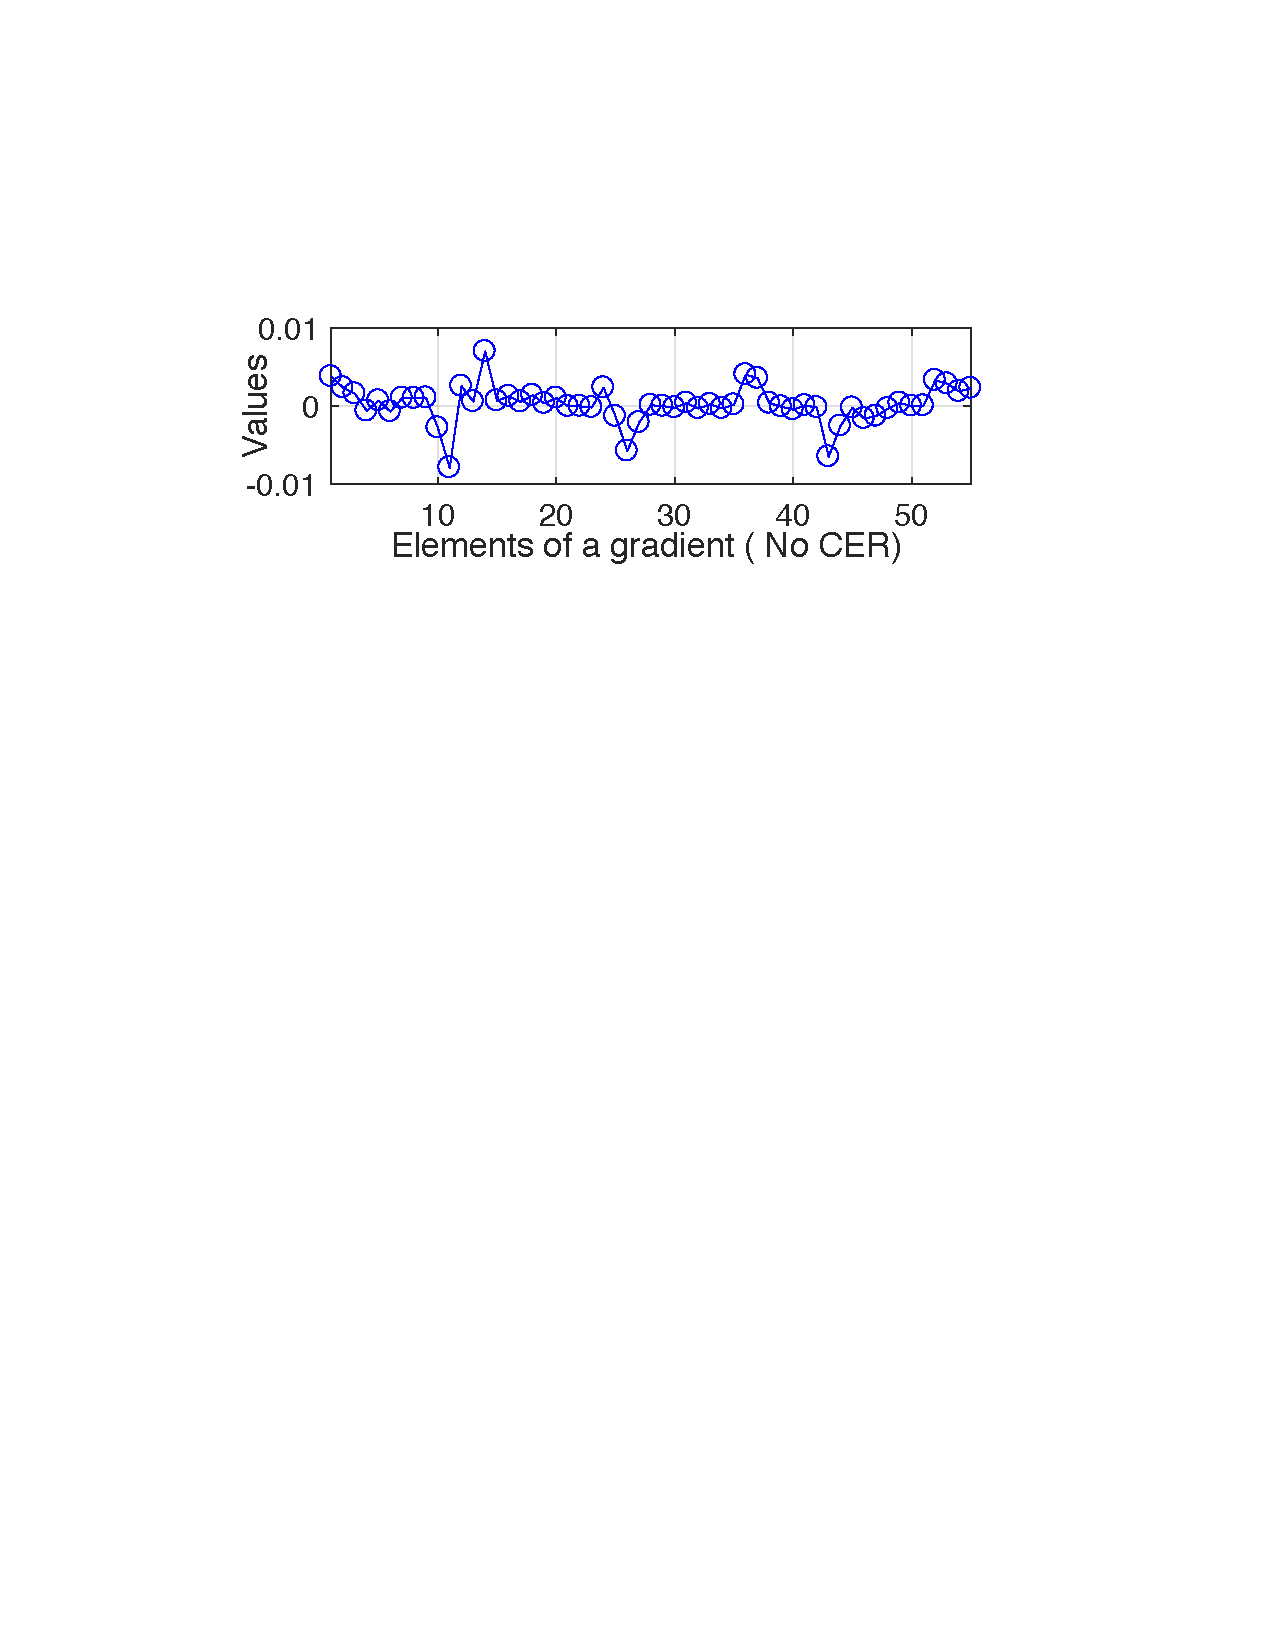
\includegraphics[width=0.47\columnwidth]{figures/figure_illustrative_communication_efficient_clustering_1}\label{figure_illustrative_communication_efficient_clustering_1}}
\subfigure{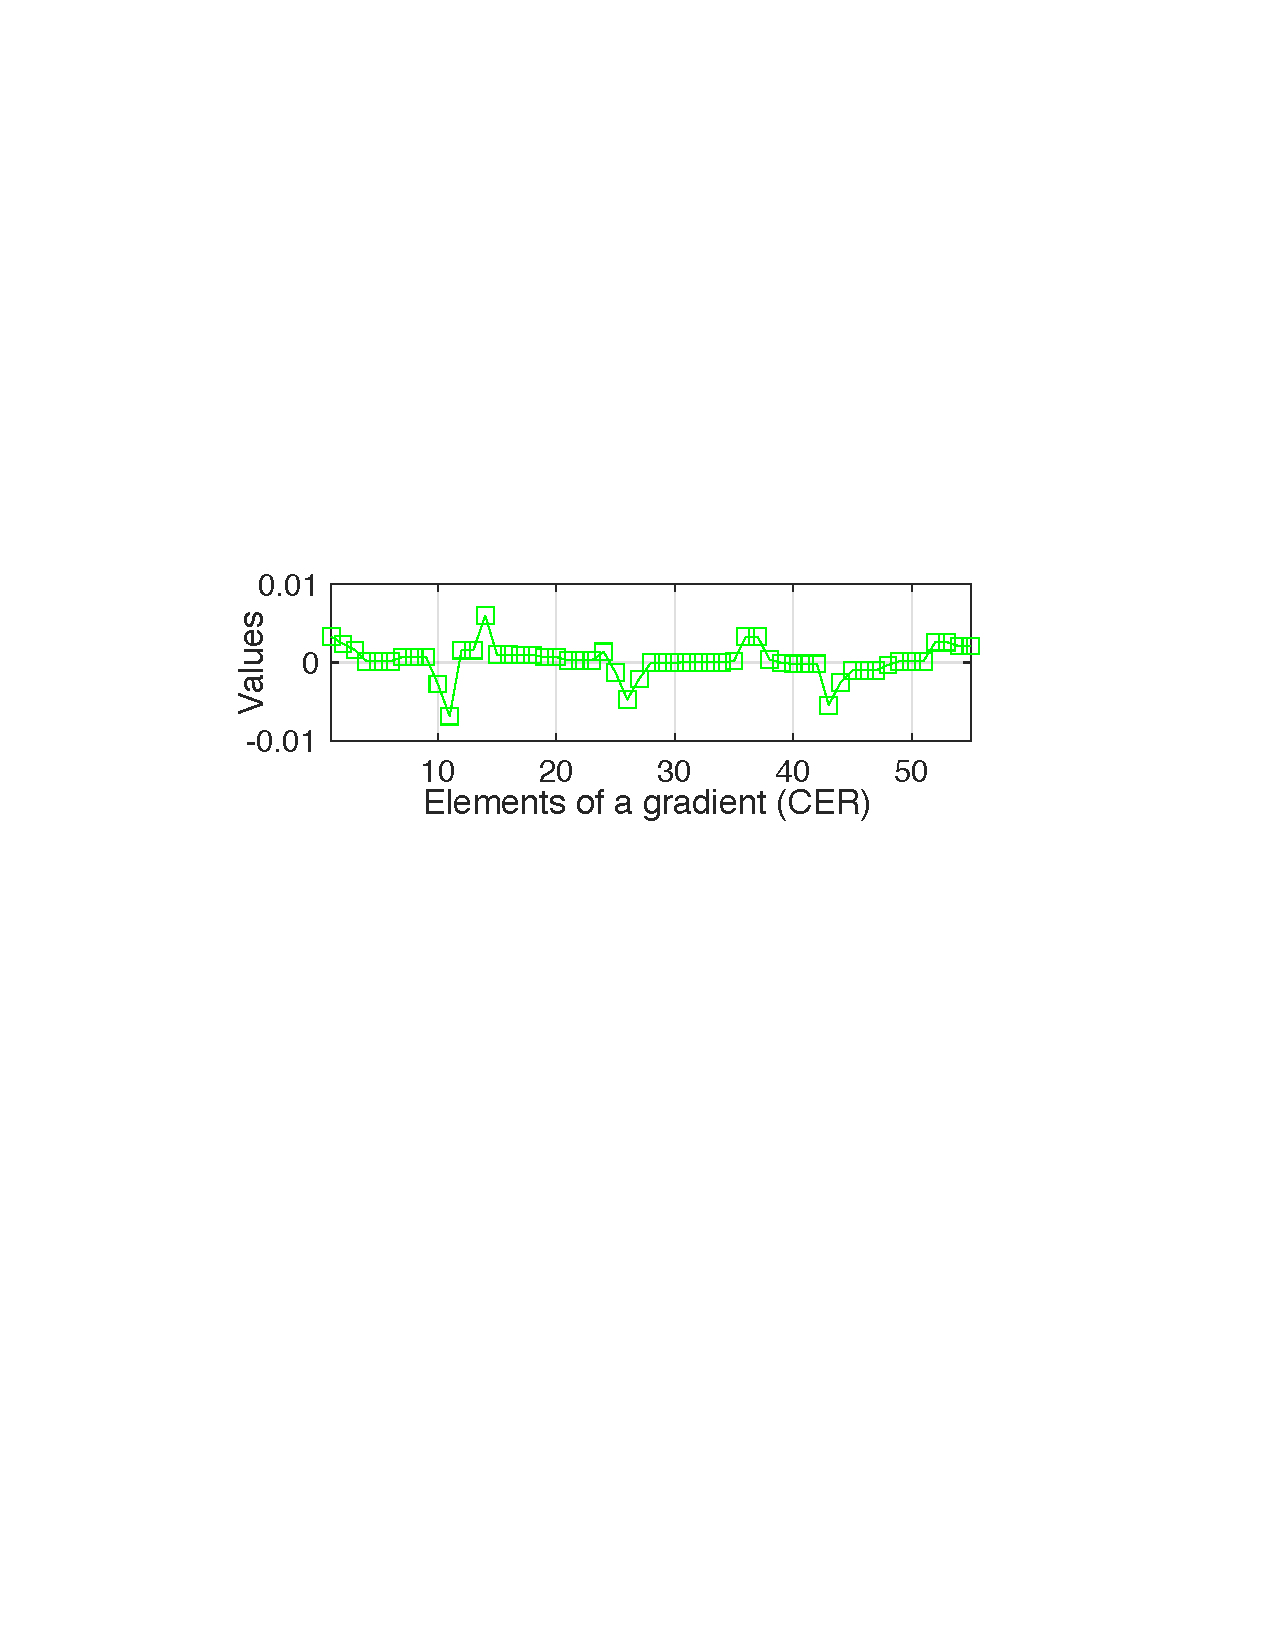
\includegraphics[width=0.47\columnwidth]{figures/figure_illustrative_communication_efficient_clustering_2}\label{figure_illustrative_communication_efficient_clustering_2}}
\subfigure{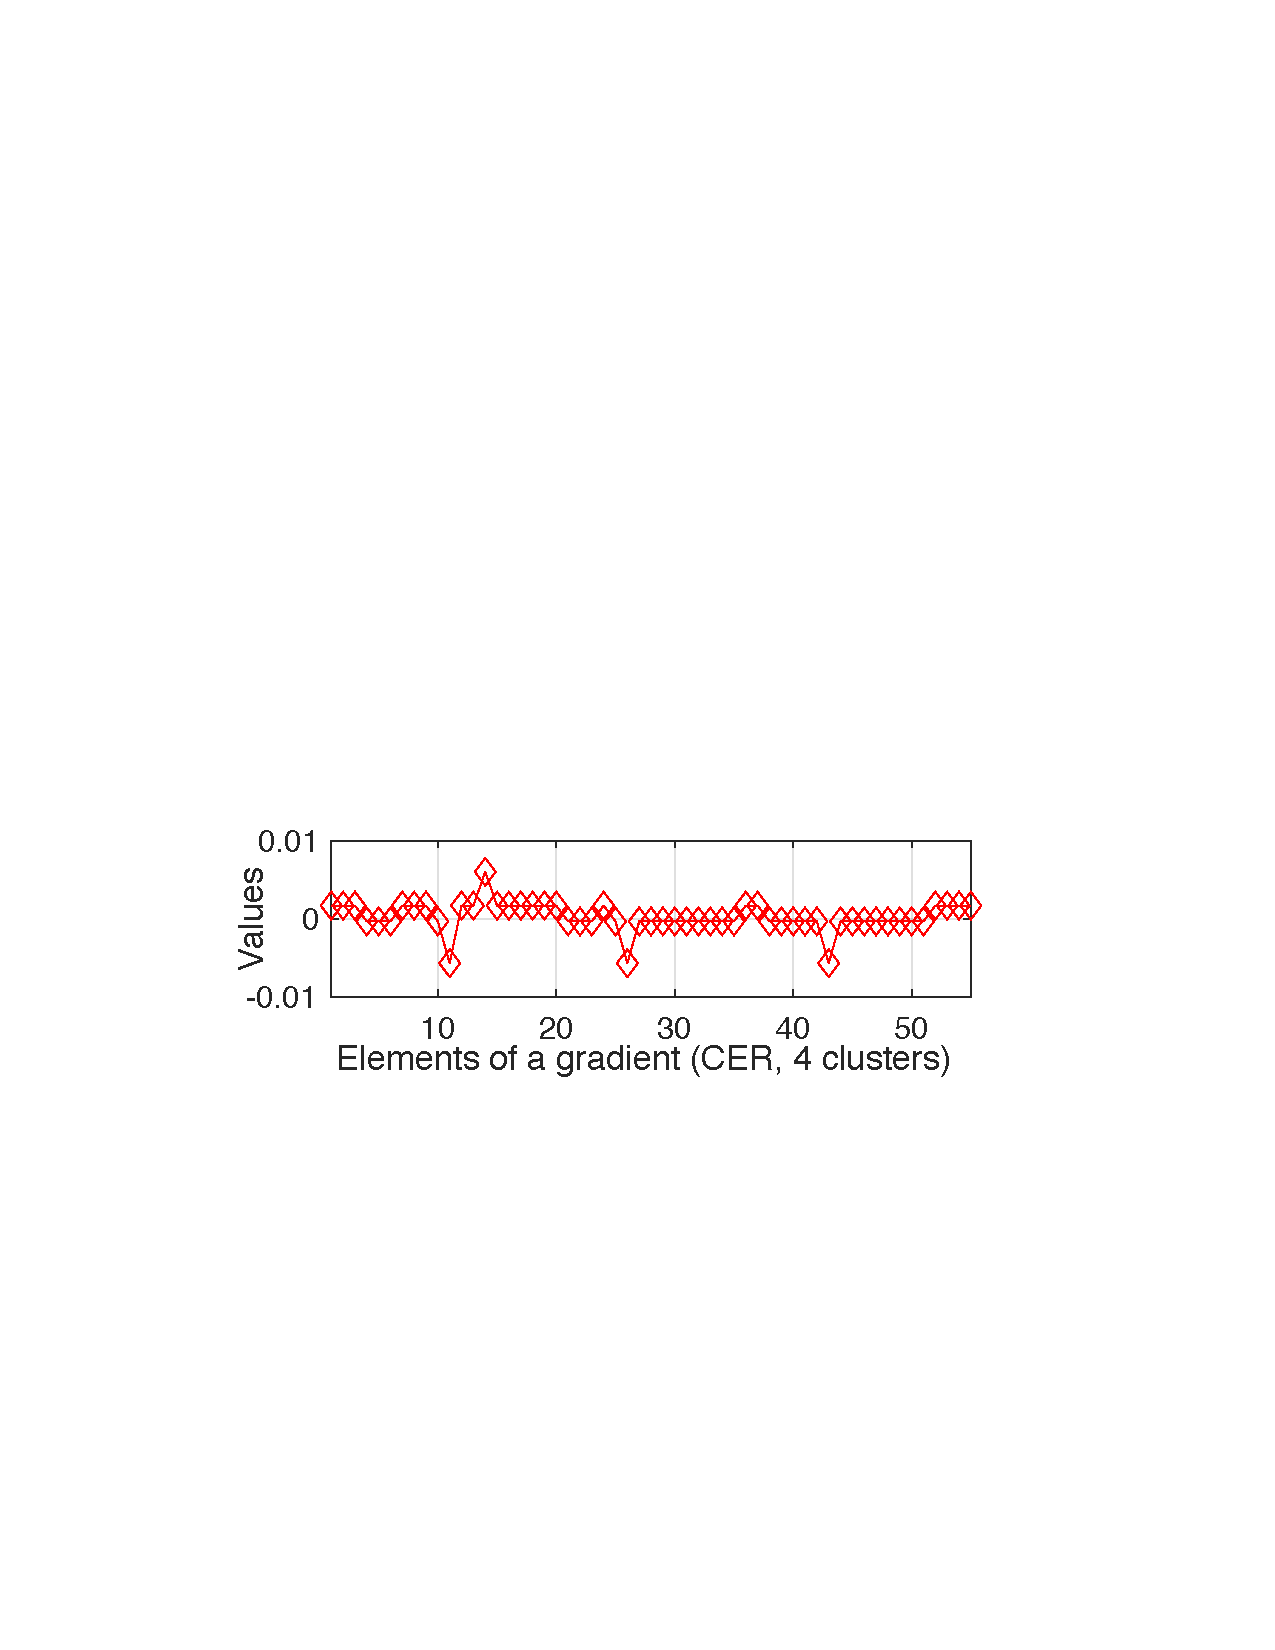
\includegraphics[width=0.47\columnwidth]{figures/figure_illustrative_communication_efficient_clustering_3}\label{figure_illustrative_communication_efficient_clustering_3}}
\subfigure{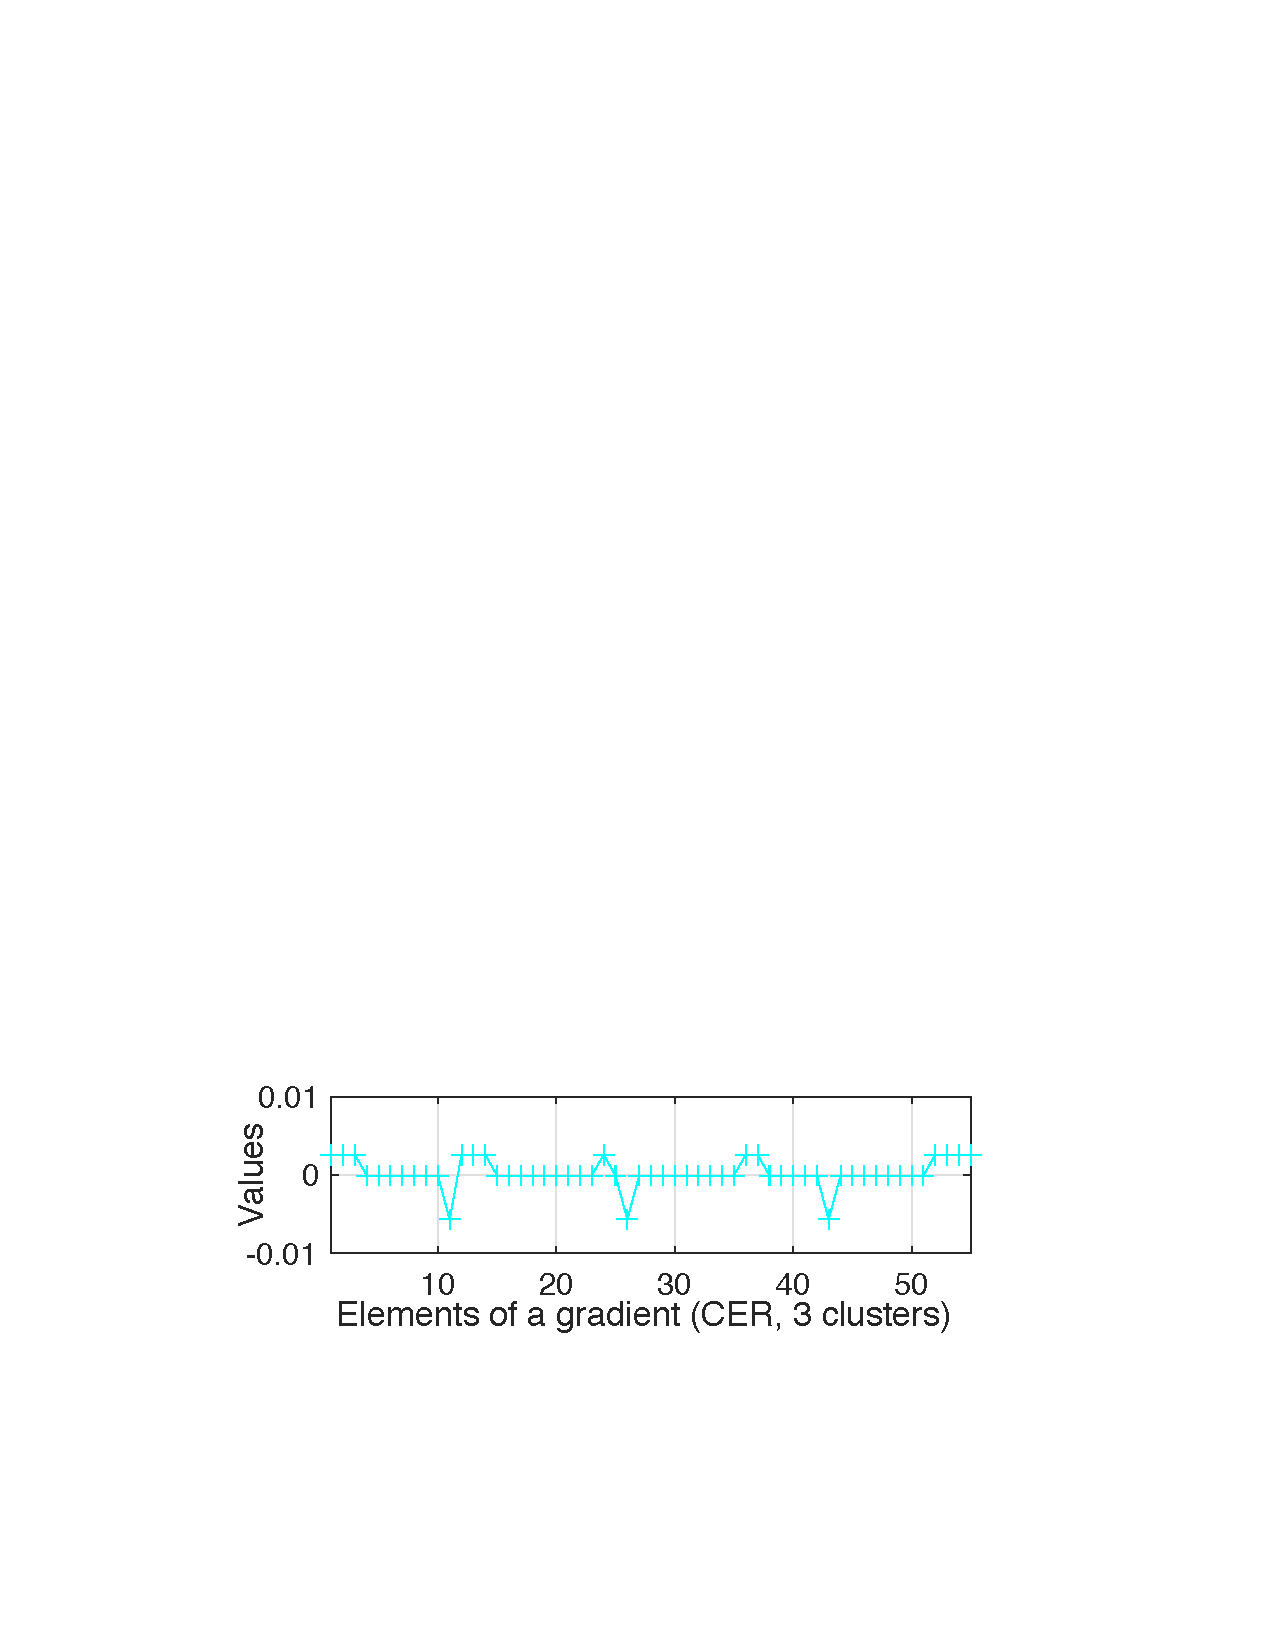
\includegraphics[width=0.47\columnwidth]{figures/figure_illustrative_communication_efficient_clustering_4}\label{figure_illustrative_communication_efficient_clustering_4}}
\caption{Comparison of elements of $\y_{t+1}^{(w)}$. The first sub-figure is plotted by using the classic gradient descent method without the Communication Efficient Regularizer (CER). The second sub-figure is plotted by using our method, i.e., Eq. \eqref{equa_update_rule_cer_distributed}. The third and fourth sub-figures are plotted by using our method and the k-means clustering coding strategy with $k=3$ and $k=4$, respectively.  }
\label{figure_illustrative_communication_efficient_clustering}
\end{figure*}






\section{Coding strategy}
\label{sect_coding_strategy}
In this section, we present some coding strategies to encode the sequence  $\{\y_t^{(w)}\}_{t=1}^T$.





As we have shown, the elements of $\y_{t+1}^{(w)}$ own some clustering structures. Exploiting the intrinsic clustering structures, it is able to encode $\y_{t+1}^{(w)}$ with few bits. We furthermore conduct clustering, e.g., k-means on elements of $\y_{t+1}^{(w)}$. Here, there is a trade-off between the accuracy and communication efficiency. When elements of a gradient are partitioned into more clusters, the higher accuracy of the gradient is guaranteed. Meanwhile, the gradient has to be encoded by using more bytes, thus leading to the decrease of the communication efficiency.  

We take an example for more explanation. We conduct logistic regression on the \textit{covtype} dataset. $\y_{t+1}^{(w)}$ has $55$ elements. As illustrated in Figure \ref{figure_illustrative_communication_efficient_clustering}, the x-axis represents the elements, and the y-axis represents values of an element. When the basic gradient descent method, i.e., Eq. \eqref{equa_sgd_local_update} is used to yield $\y_{t+1}^{(w)}$, the top-left sub-figure shows that its elements are usually different. But, when the communication efficient regularizer is used to update $\y_{t+1}^{(w)}$, the top-right sub-figure shows that its elements can be partitioned into multiple clusters.  When k-means clustering is furthermore conducted on those elements, the bottom-left and bottom-right sub-figures show that those elements can be represented with $k=4$ and $k=3$ cluster centers, respectively.  Suppose every cluster center needs $b$ bits to be encoded. Those cluster centers need $kd$ bits. Additionally, we present two method to encode the clustering membership. 
\begin{itemize}
\item  {\textbf{Elias integer encoding method.}} For every element of $\y_{t+1}^{(w)}$, we use Elias integer coding method to encode the index of its cluster \cite{elias}. The code length is not larger than $\log d + 1$.  For every cluster, the code length to represent its clustering membership is not larger than $d(\log d + 1)$. Finally, the  required code length is  not larger than $k d(\log d + 1)$.  We recommend \cite{NIPS2017_6768} for more details about the Elias integer encoding method.
\item {\textbf{Bloom filter encoding method.}} For every cluster, we use the hashing method to map its members into a sequence of bits. Every member may be mapped to more than one bits by using more than one hash functions. If a member is mapped to a bit by using a hash function, the bit will turn to $1$.  Note that bloom filter may lead to false positive error.  Suppose that the false positive probability is $p>0$, and the required code length is thus $-\frac{kd \ln p}{(\ln 2)^2}$.    We recommend \cite{bloomfilter} for more details about the Bloom filter.
\end{itemize}


\begin{figure*}[!t]
\setlength{\abovecaptionskip}{0pt}
\setlength{\belowcaptionskip}{0pt}
\centering 
\subfigure[\textit{w8a, logistic regression}]{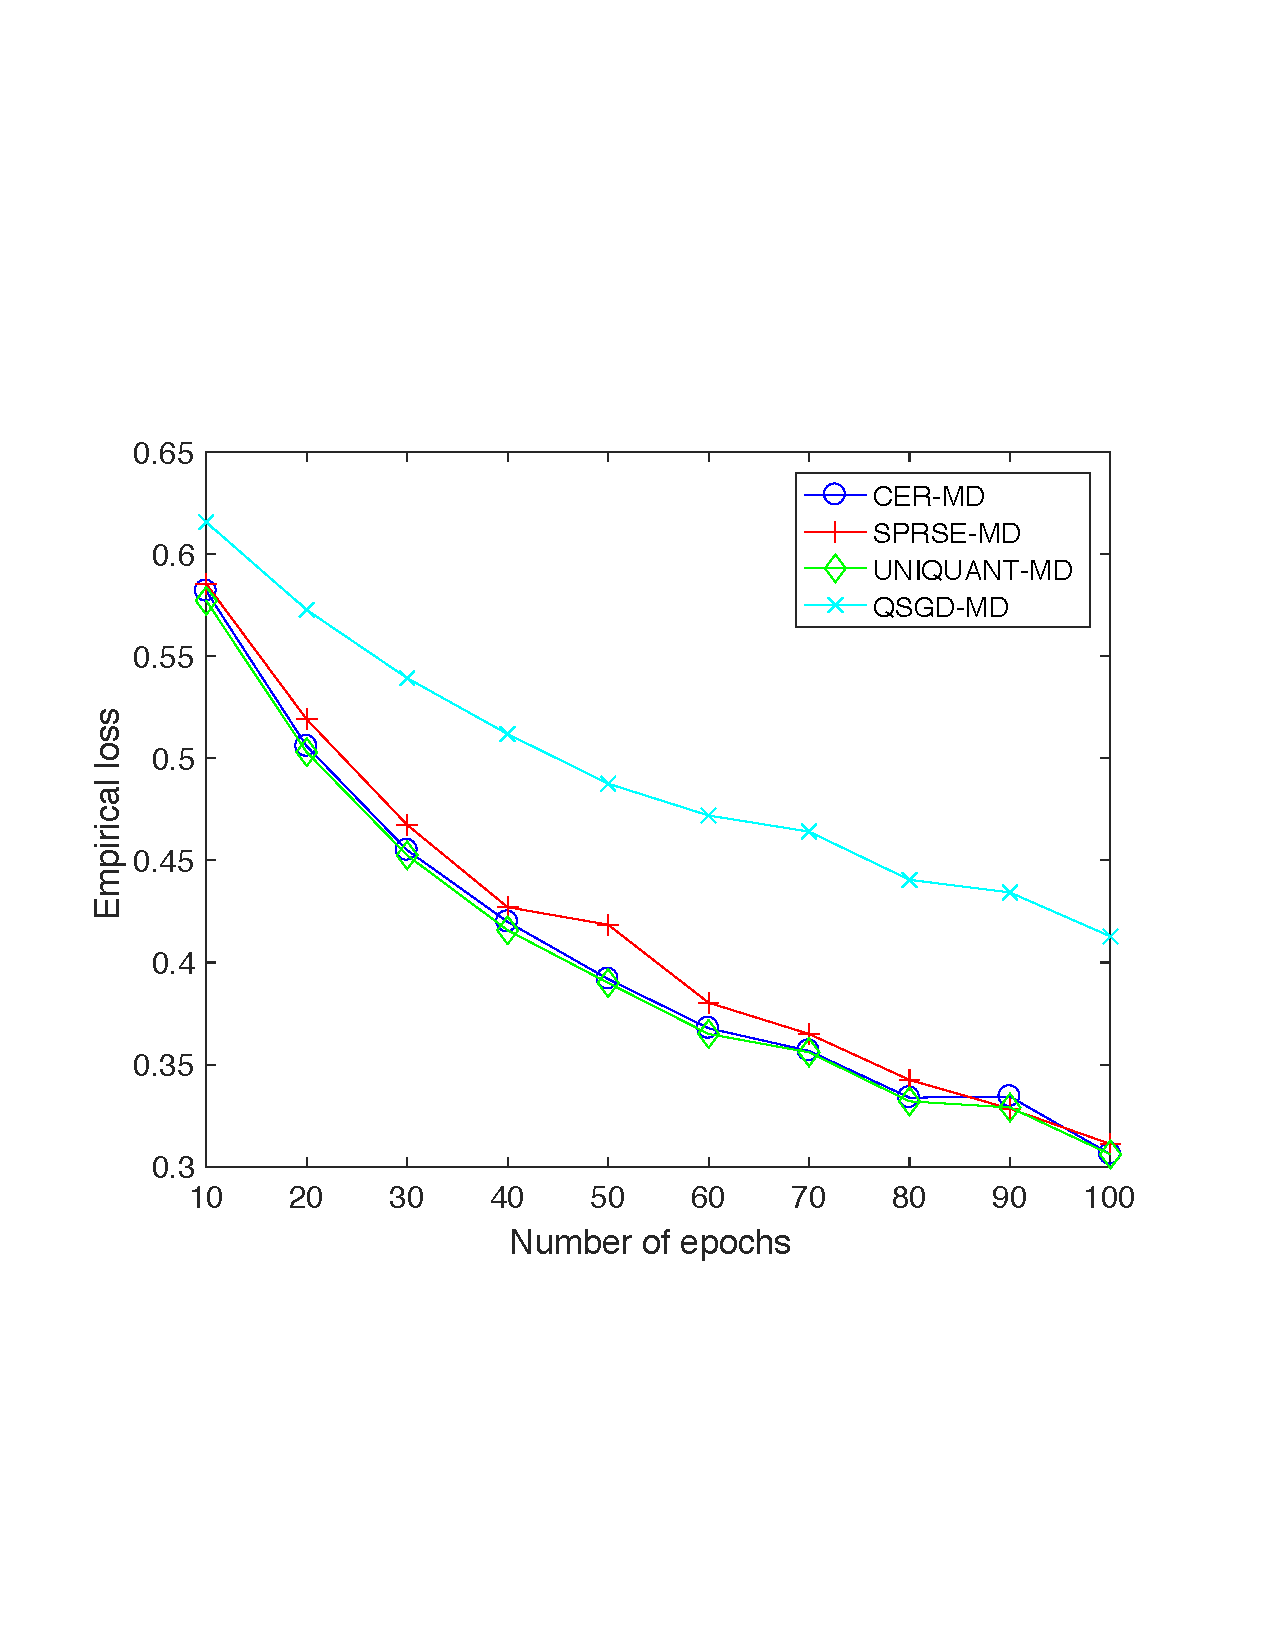
\includegraphics[width=0.32\columnwidth]{figures/figure_empirical_loss_w8a}\label{figure_empirical_loss_w8a}}
\subfigure[\textit{a9a, logistic regression}]{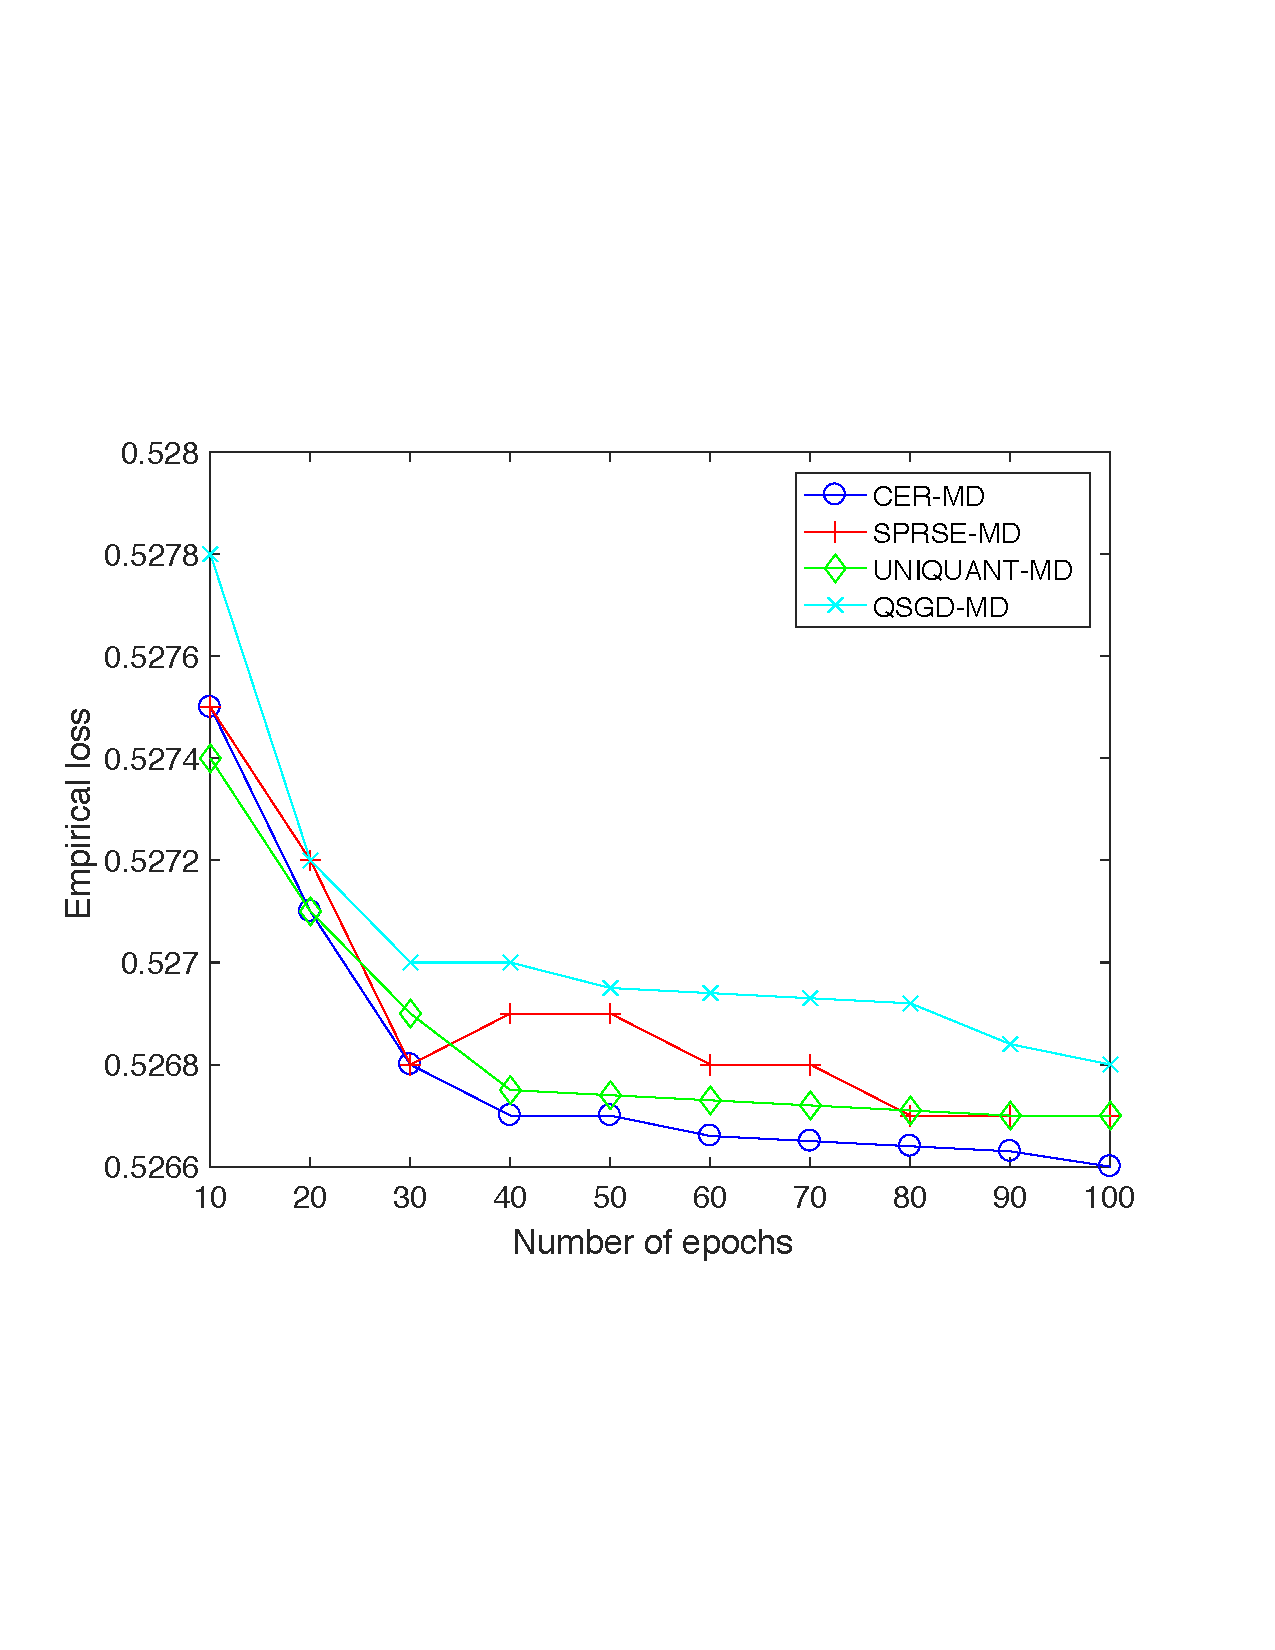
\includegraphics[width=0.33\columnwidth]{figures/figure_empirical_loss_a9a}\label{figure_empirical_loss_a9a}}
\subfigure[\textit{covtype, logistic regression}]{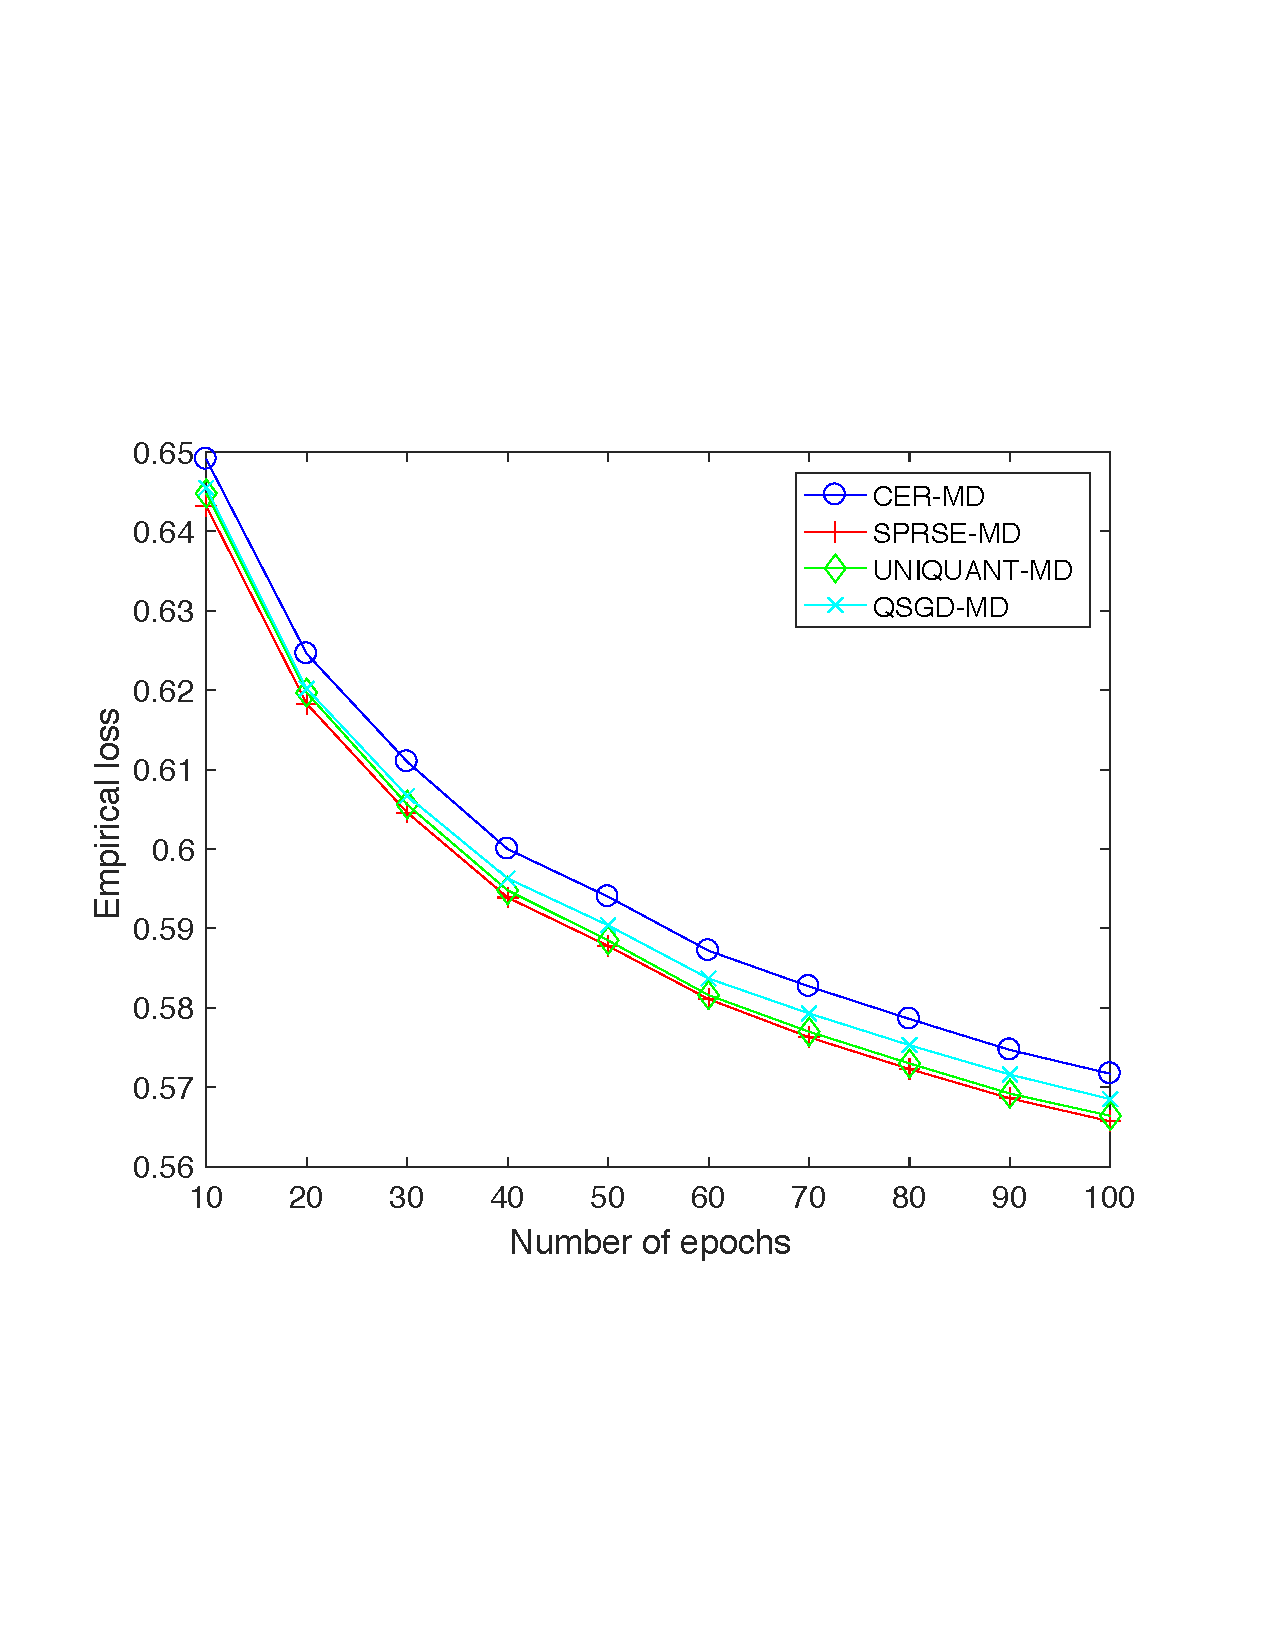
\includegraphics[width=0.32\columnwidth]{figures/figure_empirical_loss_covtype}\label{figure_empirical_loss_covtype}}
\subfigure[\textit{year, ridge regression}]{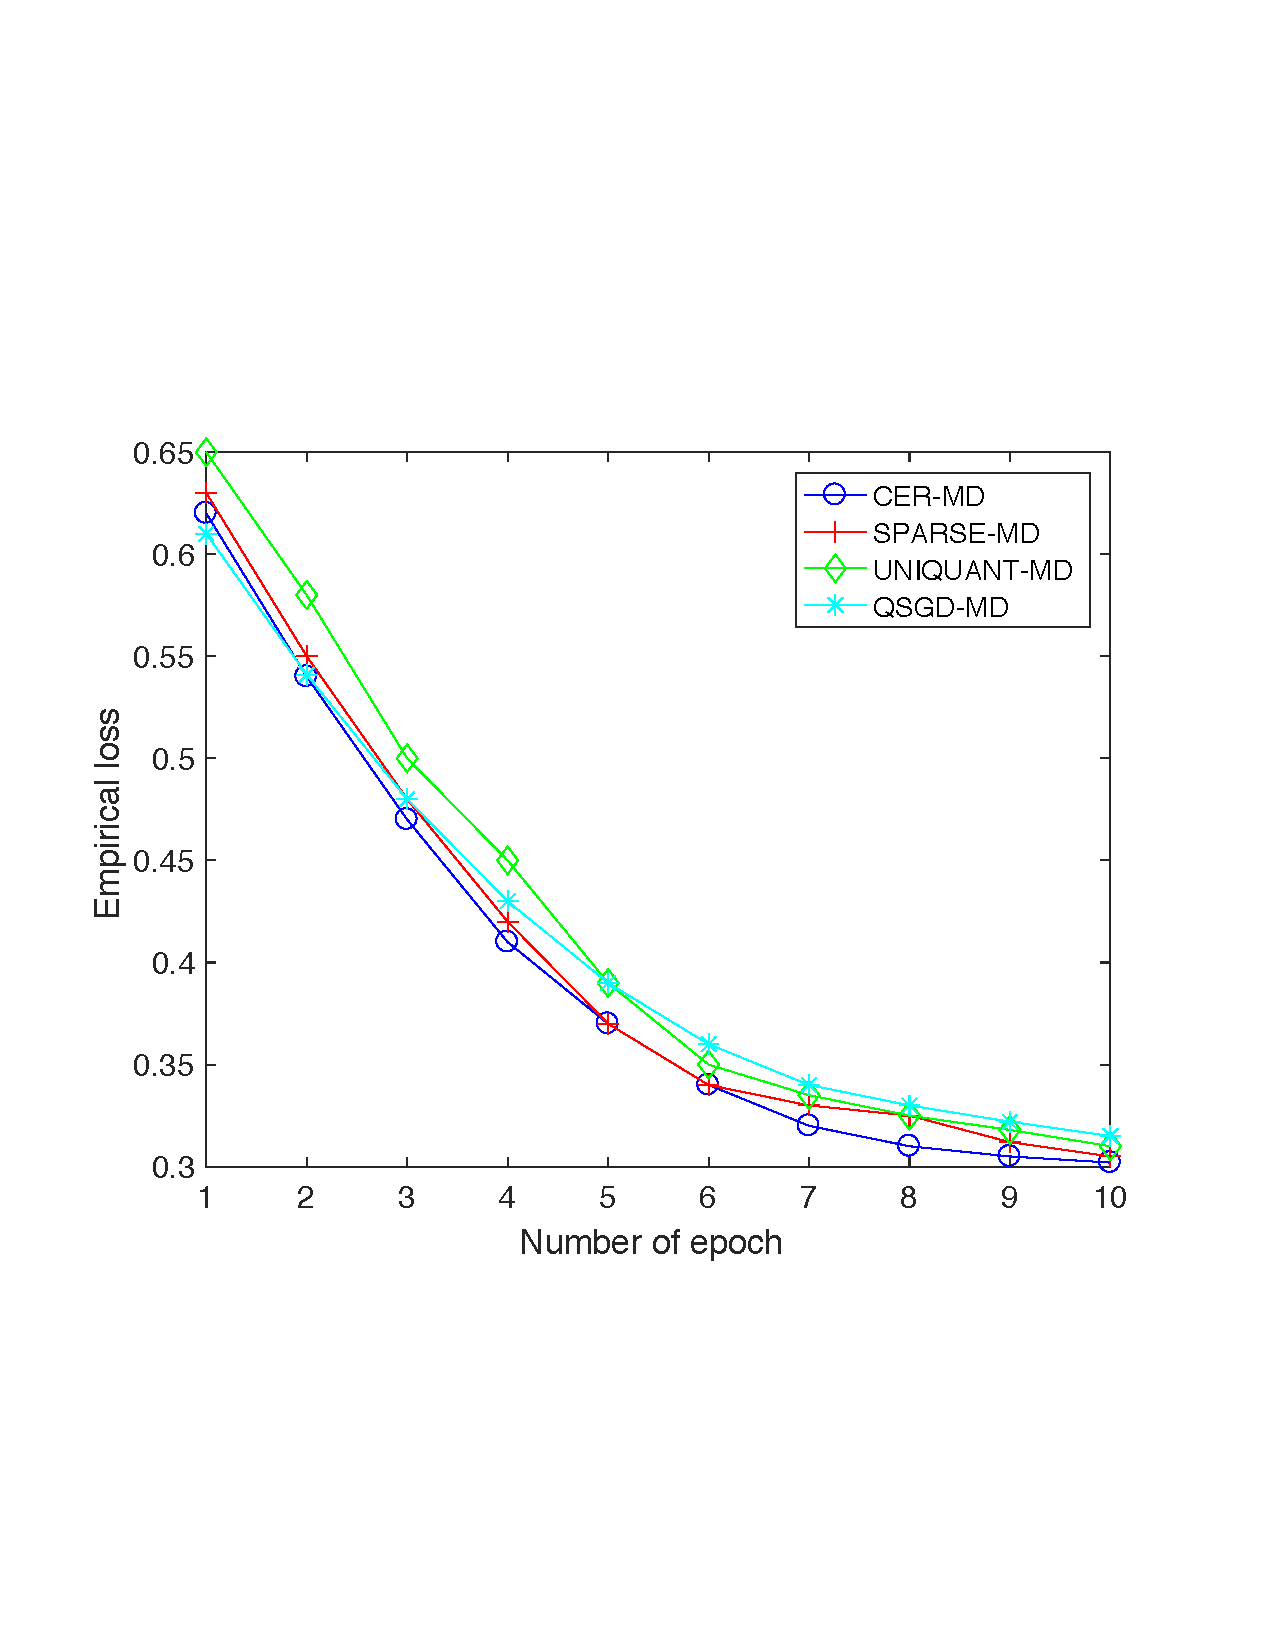
\includegraphics[width=0.325\columnwidth]{figures/figure_empirical_loss_year}\label{figure_empirical_loss_year}}
\subfigure[\textit{cadata, ridge regression}]{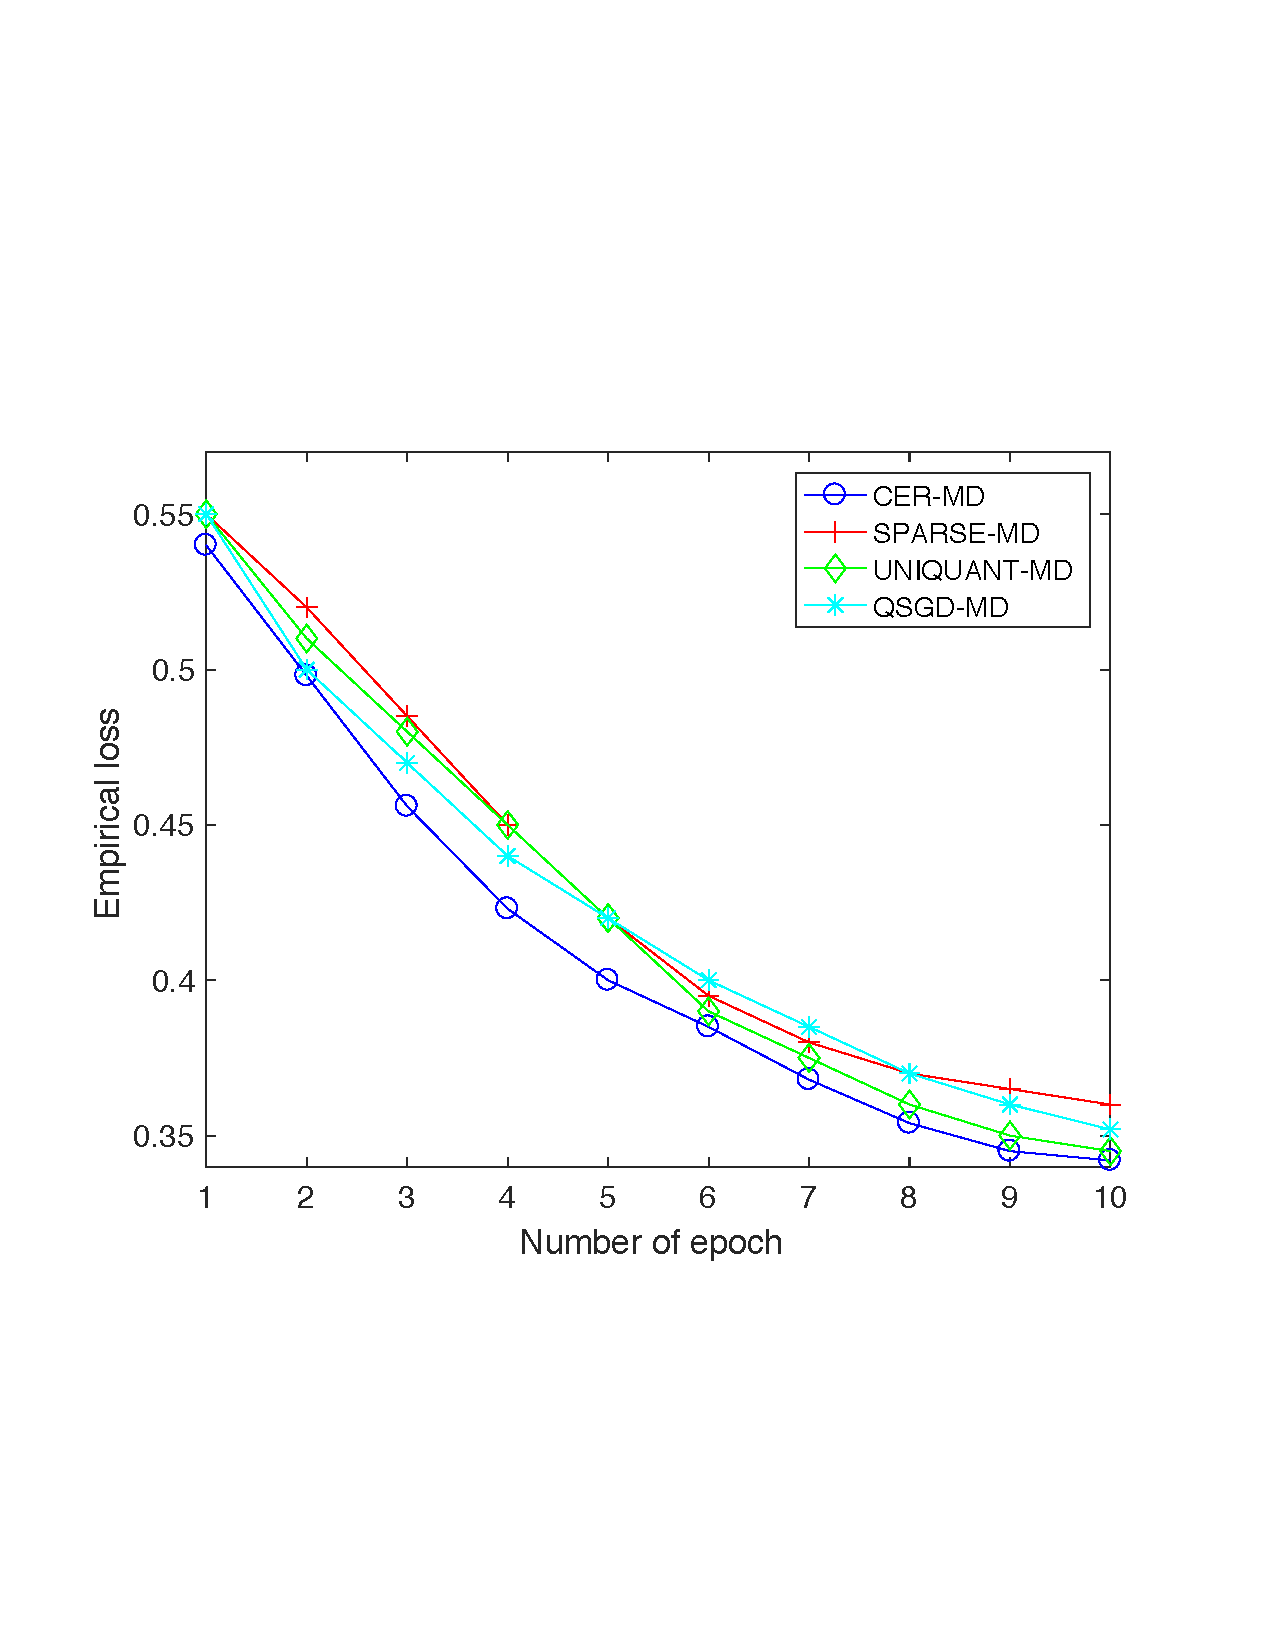
\includegraphics[width=0.32\columnwidth]{figures/figure_empirical_loss_cadata}\label{figure_empirical_loss_cadata}}
\subfigure[\textit{cpusmall, ridge regression}]{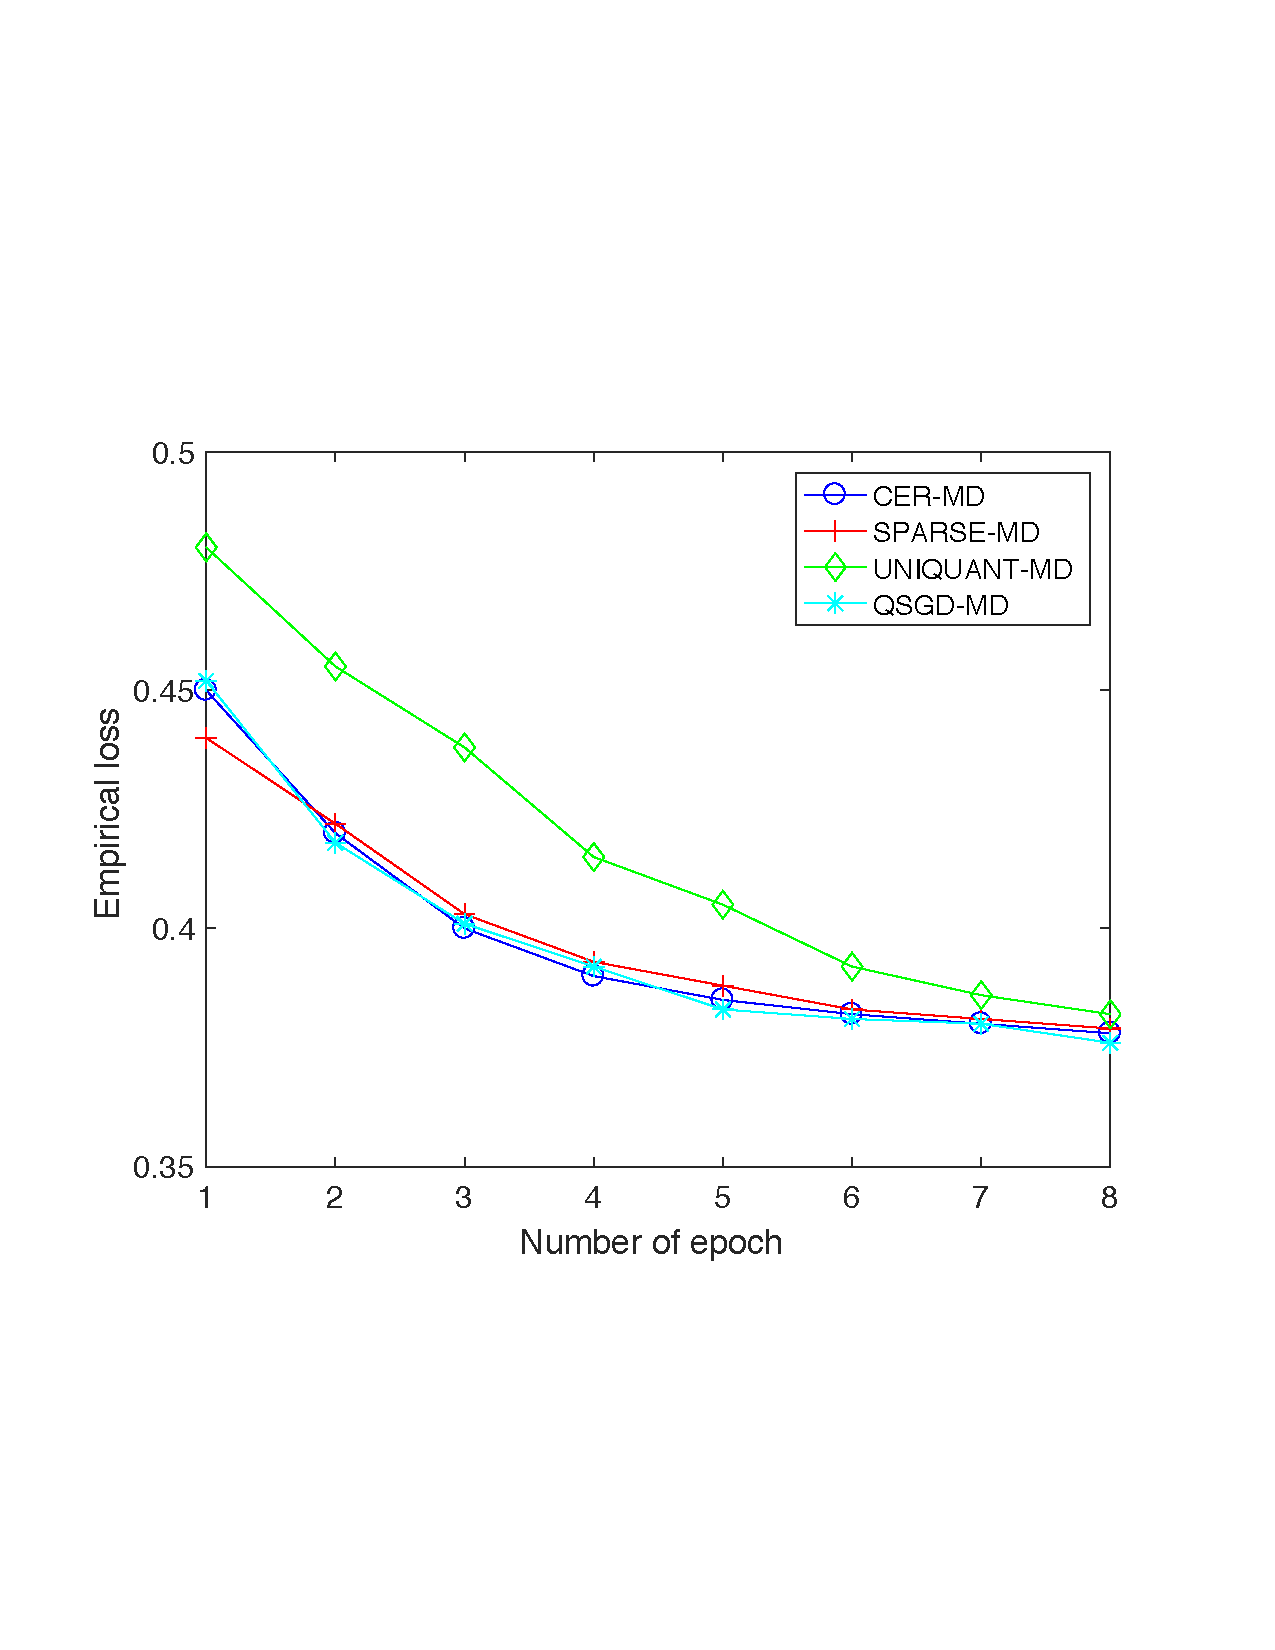
\includegraphics[width=0.32\columnwidth]{figures/figure_empirical_loss_cpusmall}\label{figure_empirical_loss_cpusmall}}
\caption{Comparsion of the empirical loss. Our method \textit{CER-MD} obtains the comparable convergence performance with the state-of-the-art methods.}
\label{figure_empirical_loss_logistic_regression}
\end{figure*}


\section{Empirical studies}
\label{sect_experiment}


\subsection{Experimental settings}
\label{subsect_experiment_settings}

We conduct classification tasks via \textit{logistic regression} and prediction tasks \textit{ridge regression} to evaluate the proposed method. The formulation of the logistic regression is $\min_{\x\in\RR^d} \frac{1}{M} \sum_{i=1}^M \log(1+\exp(-\y_i\A_i\x))$.  The formulation of the ridge regression is $\min_{\x\in\RR^d} \frac{1}{M} \sum_{i=1}^M \lrnorm{\A\x - \y_i }^2 + \gamma \lrnorm{\x}^2  $.   Here, $M$ represents the number of instances, $\A_i$ and $\y_i$ represent the $i$-th instance and its label, respectively. $\gamma$ is a hyper-parameter which is given before conducting the task. Those two tasks are implemented by using  the parameter server system \textit{DMTK} \cite{dmtk}.  The parameter server system is deployed by using five computing machines (four workers and one server).    

We conduct the logistic regression on datasets: \textit{w8a}\footnote{https://www.csie.ntu.edu.tw/$\sim$cjlin/libsvmtools/datasets/binary.html\#w8a}, \textit{a9a}\footnote{https://www.csie.ntu.edu.tw/$\sim$cjlin/libsvmtools/datasets/binary.html\#a9a}, and  \textit{covtype} \footnote{https://www.csie.ntu.edu.tw/$\sim$cjlin/libsvmtools/datasets/binary.html\\ \#covtype.binary}, and conduct ridge regression on datasets: \textit{year} \footnote{https://www.csie.ntu.edu.tw/$\sim$cjlin/libsvmtools/datasets/regression.html\\ \#YearPredictionMSD }, \textit{cadata} \footnote{https://www.csie.ntu.edu.tw/$\sim$cjlin/libsvmtools/datasets/regression.html\\ \#cadata} and \textit{cpusmall} \footnote{https://www.csie.ntu.edu.tw/$\sim$cjlin/libsvmtools/datasets/regression.html\\ \#cpusmall} The statics of those datasets are presented in Table \ref{table_dataset_statics}. Additionally, our method is denoted by \textit{CER-MD}, and the compared algorithms are presented as follows.
\begin{itemize}
\item \textbf{SPARSE-MD.} It proposes a gradient sparsification method to compress gradients \cite{Wangni:2017vj}.
\item \textbf{UNIQUANT-MD. } It uses the uniformly random quantization method to compress gradients \cite{Zhang:2016wx}. 
\item \textbf{QSGD-MD.} It proposes a new gradient quantization and coding method to compress gradient. \cite{NIPS2017_6768}.
\end{itemize}





\begin{table}[!h]
\centering
\caption{Statistics of datasets. }
\begin{tabular}{c|c|c|c}
\hline 
datasets & instances & features & tasks \tabularnewline
\hline 
\hline 
\textit{w8a} & $49,749$ & $300$ & clssification, logistic regression\tabularnewline
\hline 
\textit{a9a} & $32,561$ & $123$ & clssification, logistic regression\tabularnewline
\hline 
\textit{covtype} & $581,012$ & $54$ & clssification, logistic regression\tabularnewline
\hline 
\textit{year} & $463,715$ & $90$ & prediction, ridge regression\tabularnewline
\hline 
\textit{cadata} & $20,640$ & $8$ & prediction, ridge regression\tabularnewline
\hline 
\textit{cpusmall} & $8192$ & $12$ & prediction, ridge regression\tabularnewline
\hline 
\end{tabular}
\label{table_dataset_statics}
\end{table}


\begin{figure*}[!t]
\setlength{\abovecaptionskip}{0pt}
\setlength{\belowcaptionskip}{0pt}
\centering 
\subfigure[\textit{w8a, logistic regression}]{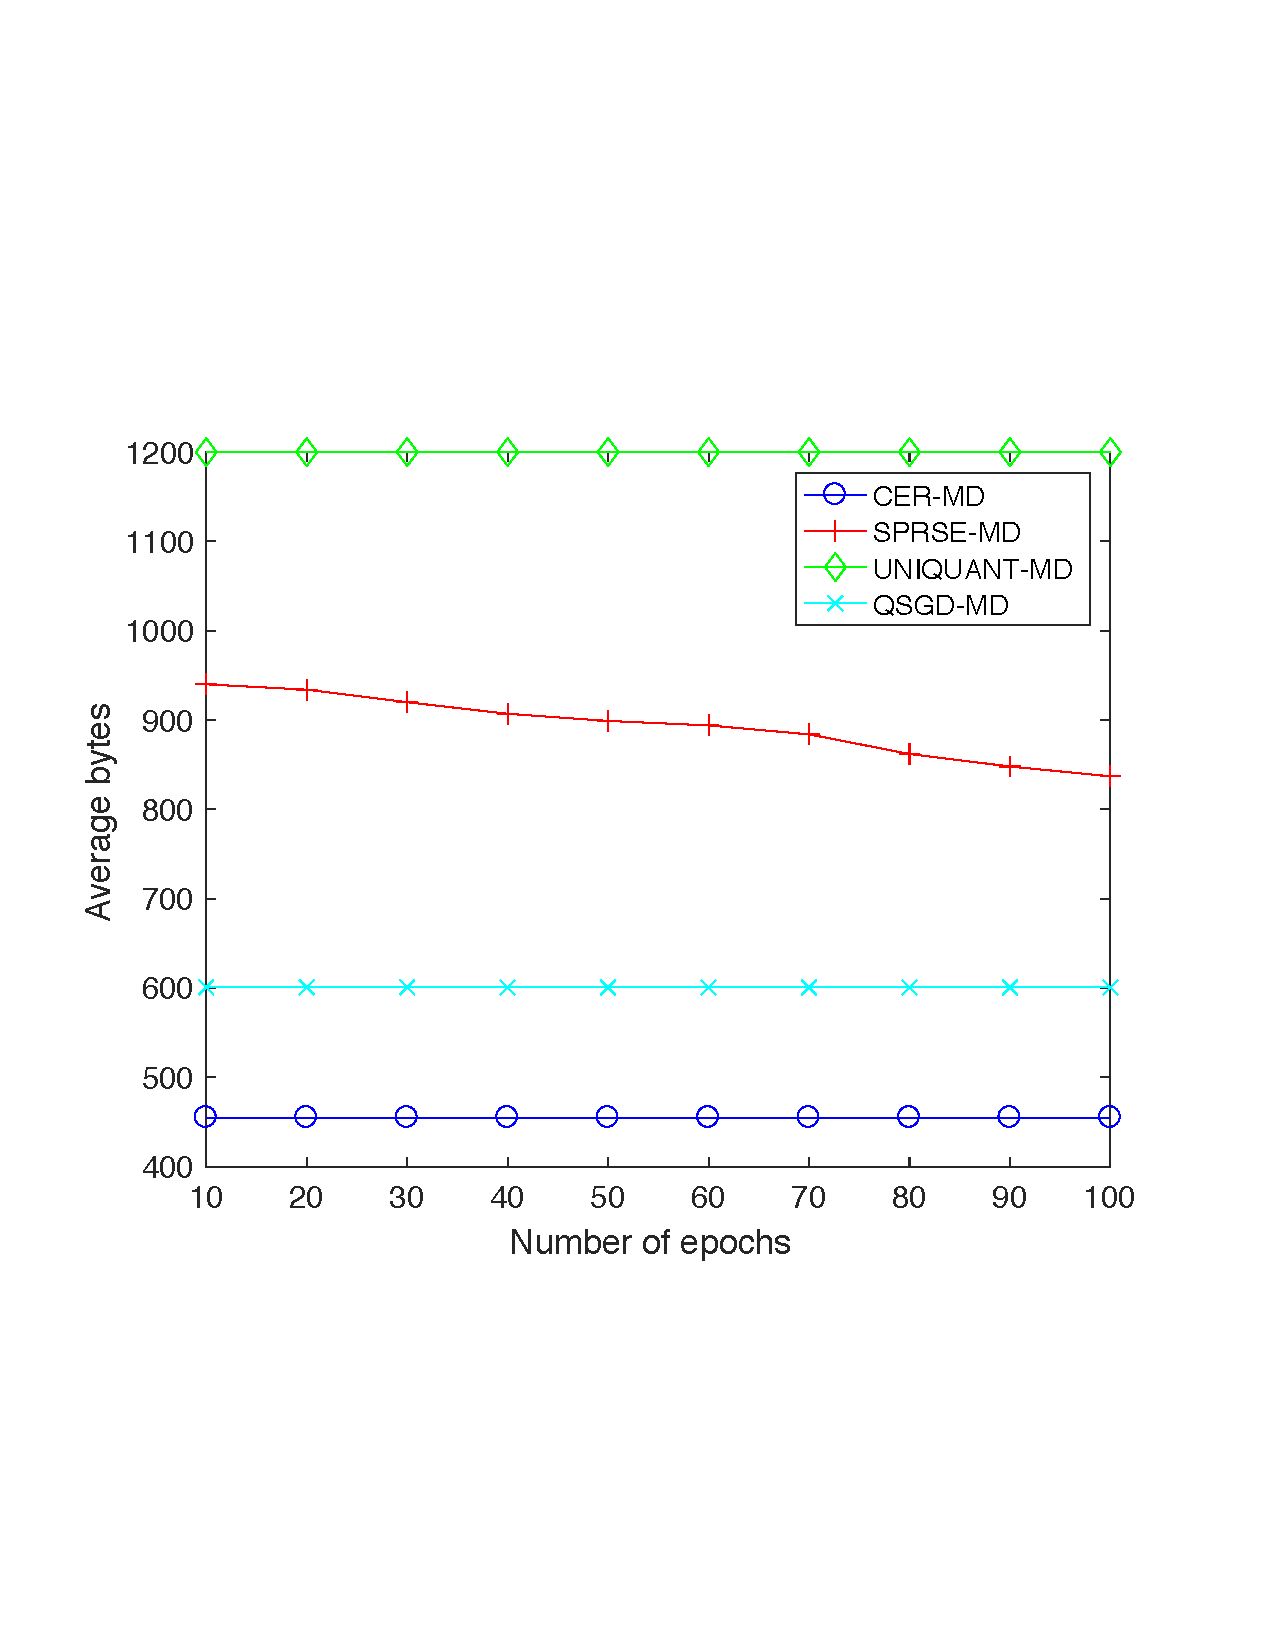
\includegraphics[width=0.32\columnwidth]{figures/figure_average_bytes_w8a}\label{figure_average_bytes_w8a}}
\subfigure[\textit{a9a, logistic regression}]{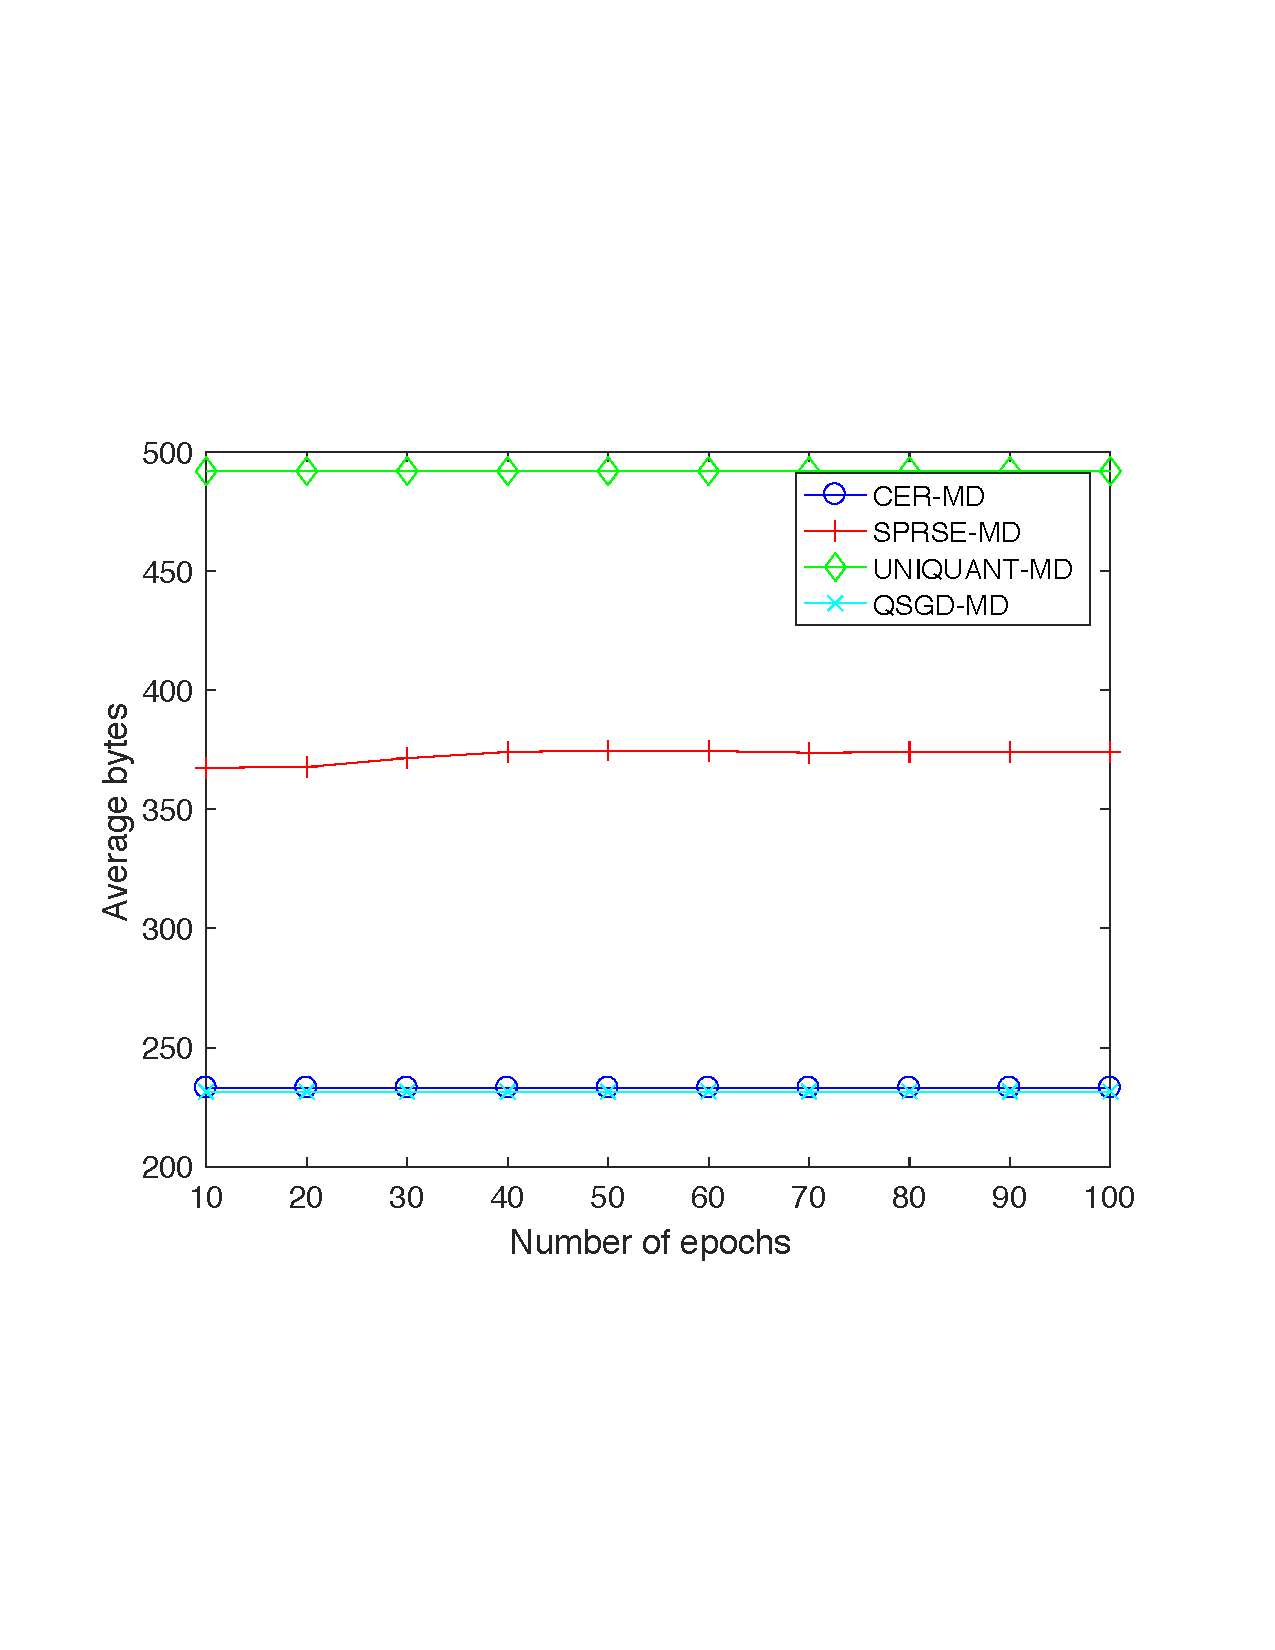
\includegraphics[width=0.32\columnwidth]{figures/figure_average_bytes_a9a}\label{figure_average_bytes_a9a}}
\subfigure[\textit{covtype, logistic regression}]{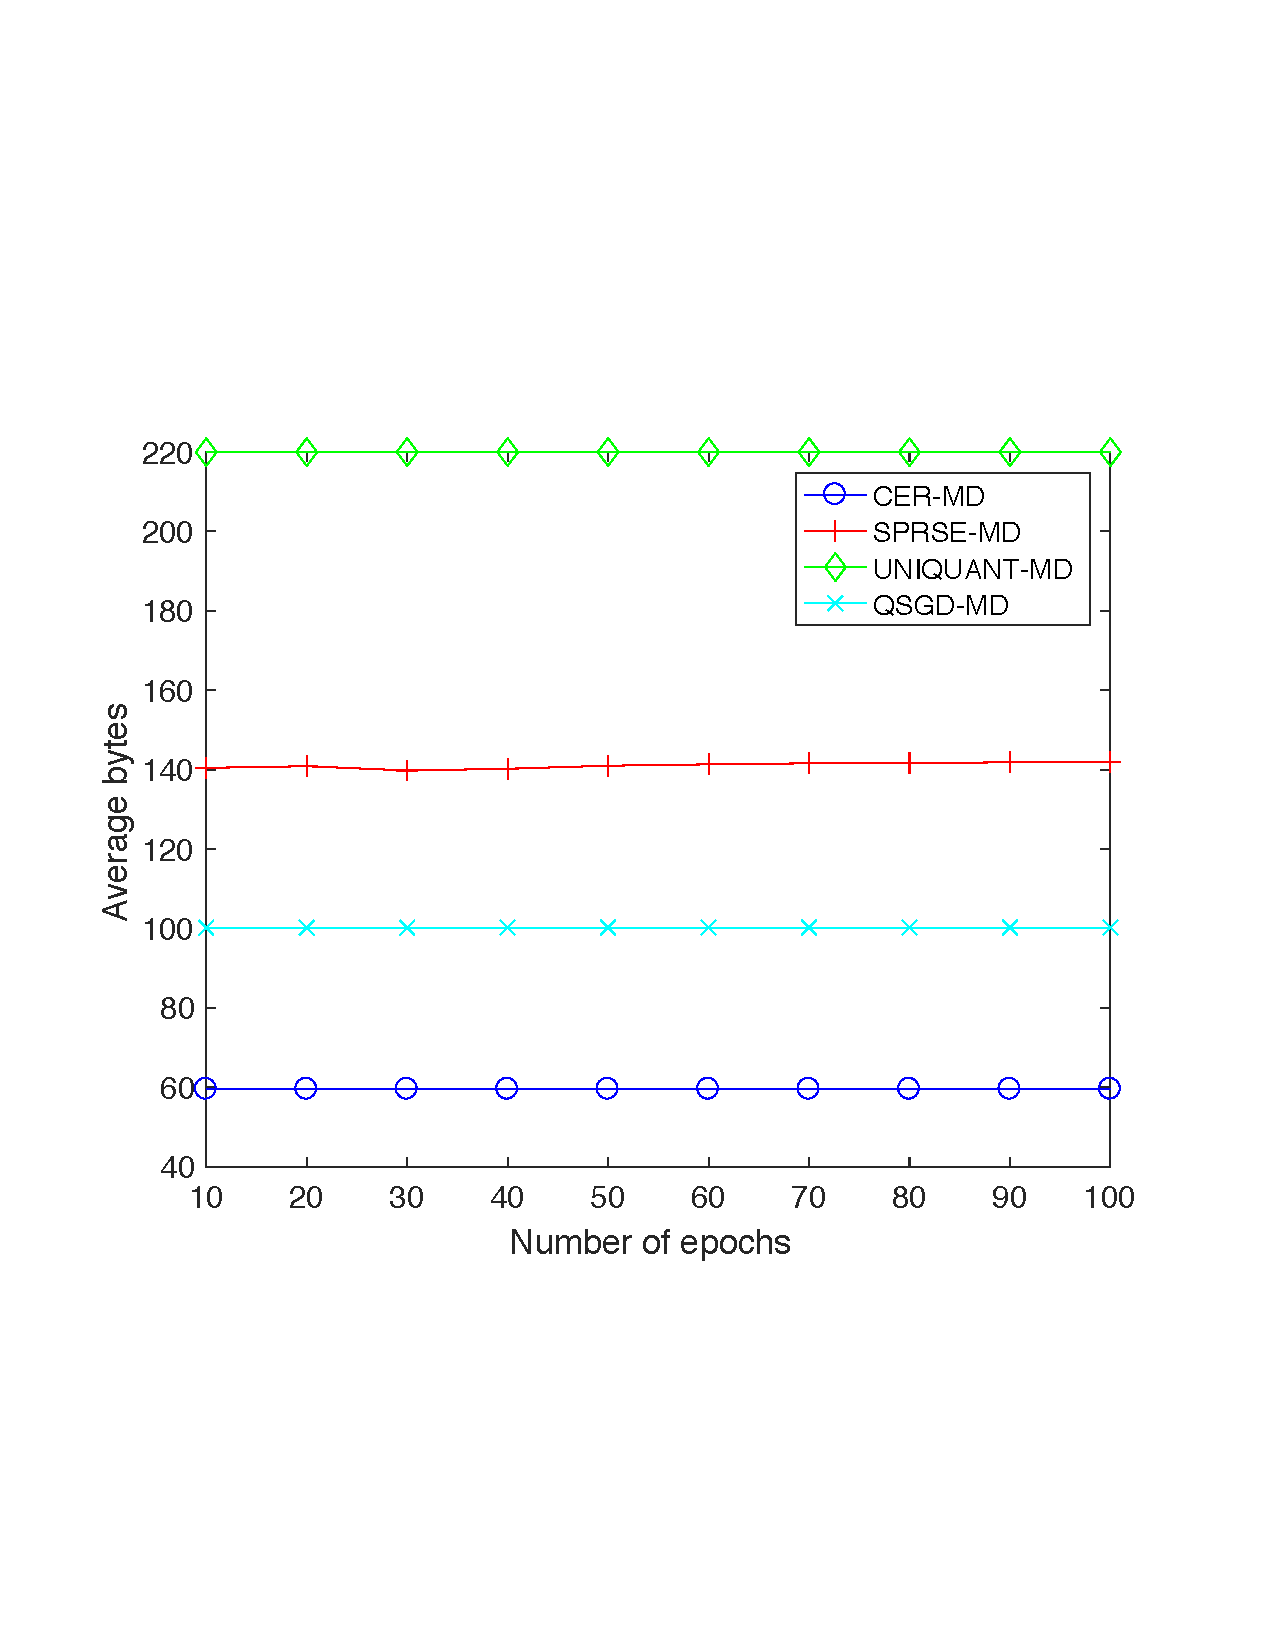
\includegraphics[width=0.32\columnwidth]{figures/figure_average_bytes_covtype}\label{figure_average_bytes_covtype}}
\subfigure[\textit{year, ridge regression}]{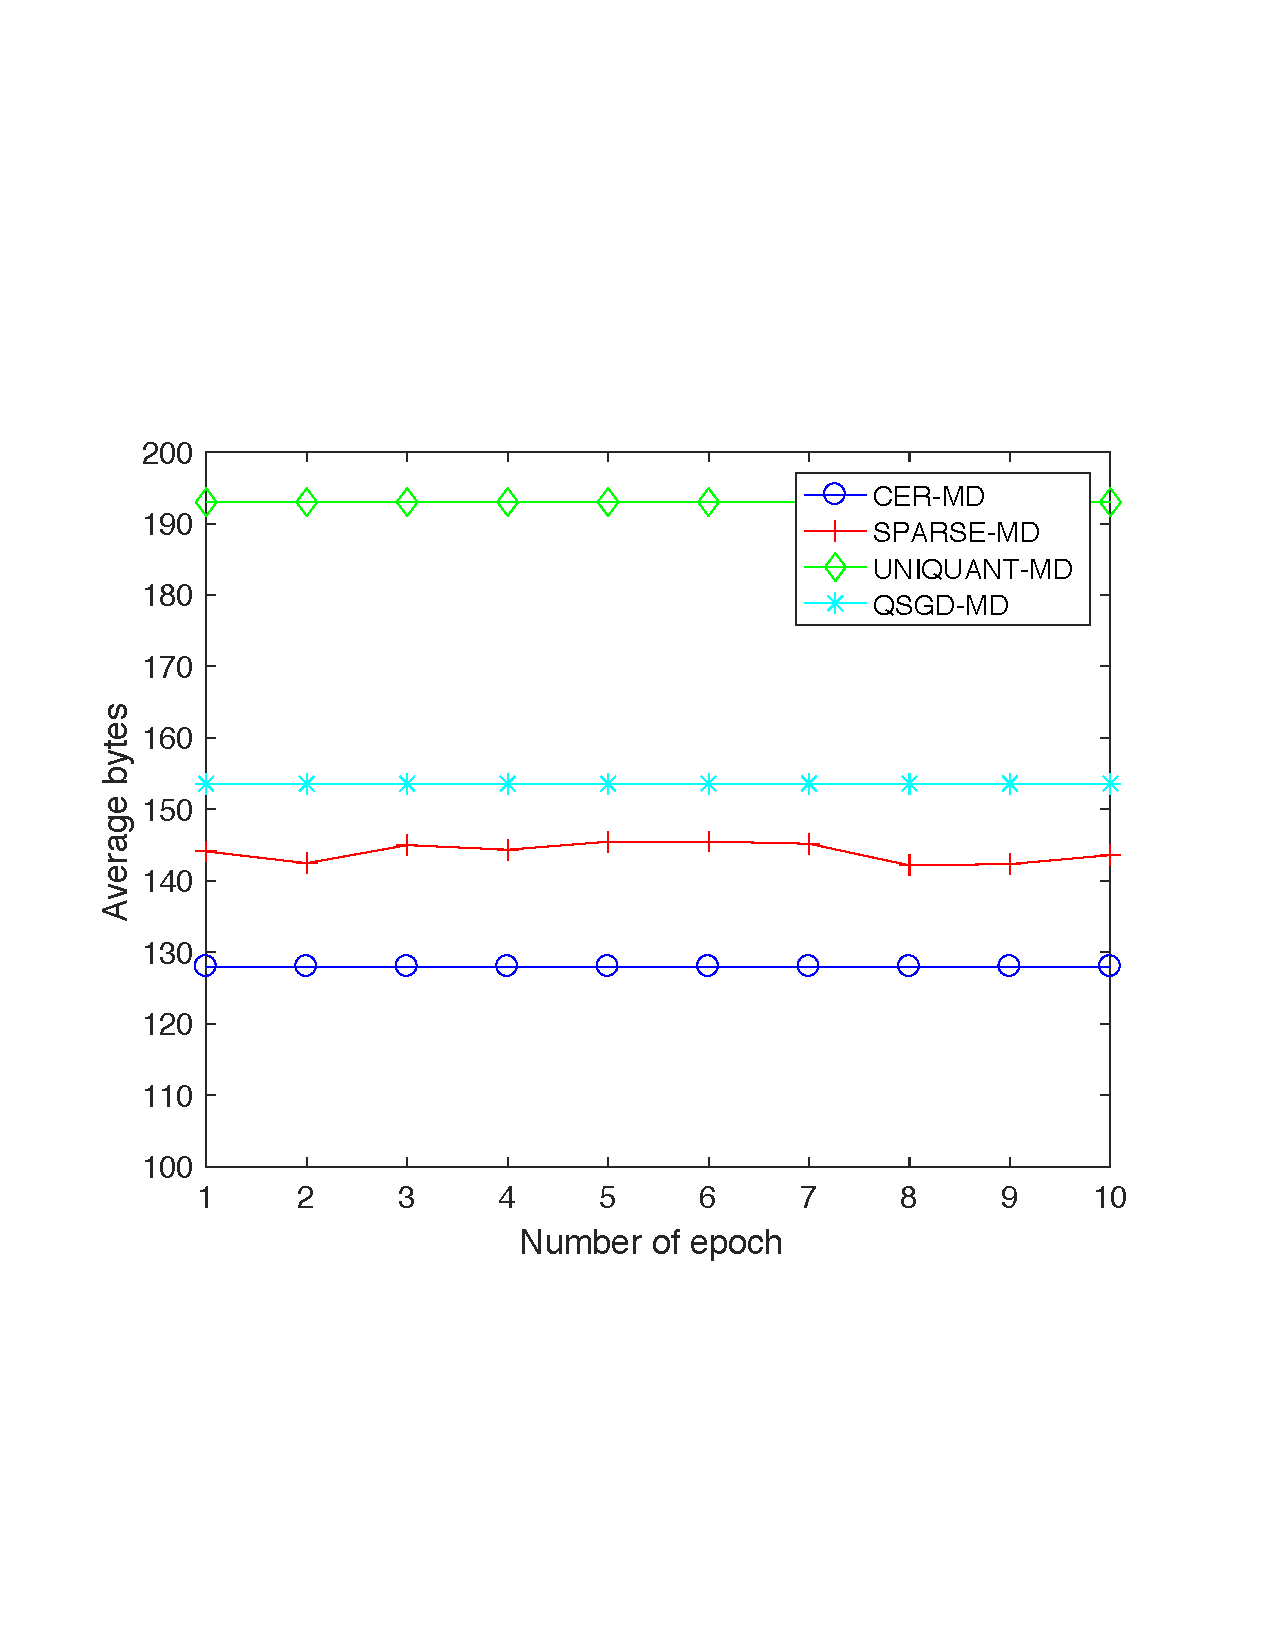
\includegraphics[width=0.33\columnwidth]{figures/figure_average_bytes_year}\label{figure_average_bytes_year}}
\subfigure[\textit{cadata, ridge regression}]{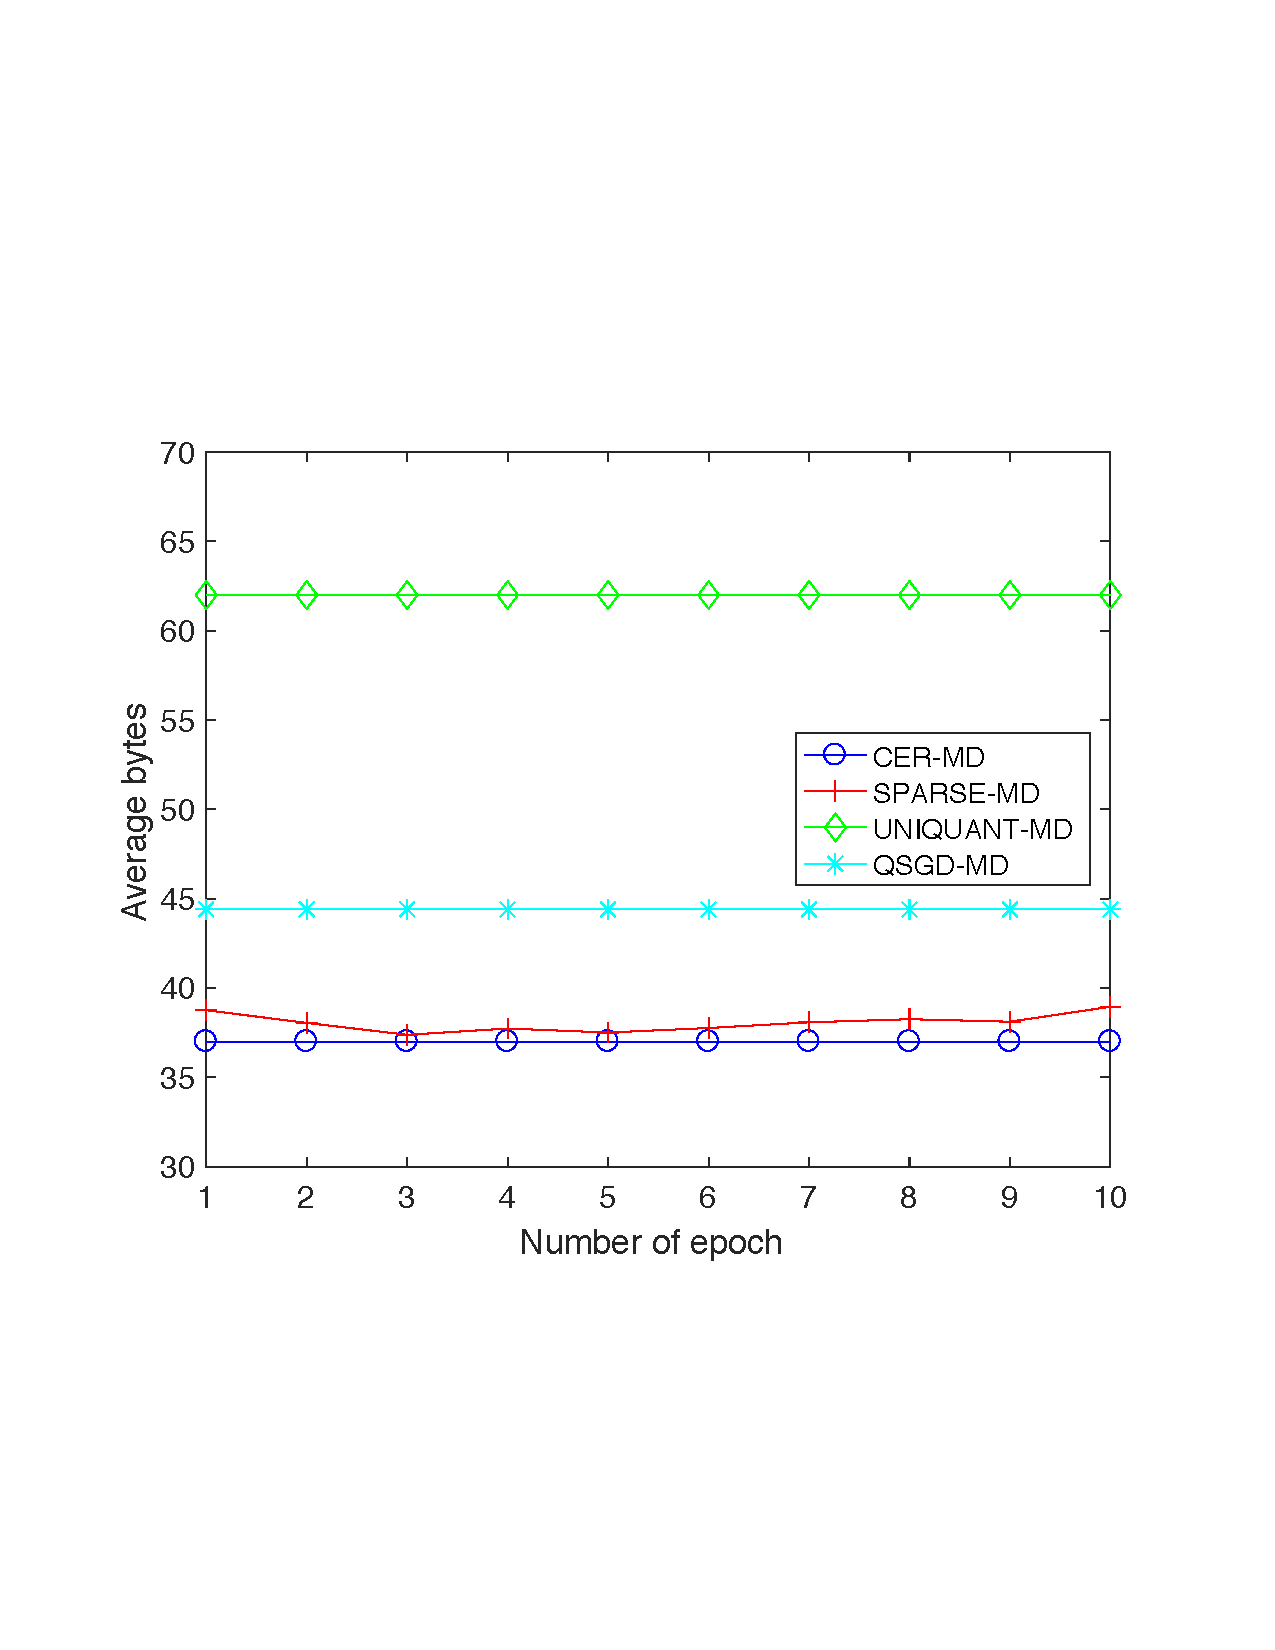
\includegraphics[width=0.32\columnwidth]{figures/figure_average_bytes_cadata}\label{figure_average_bytes_cadata}}
\subfigure[\textit{cpusmall, ridge regression}]{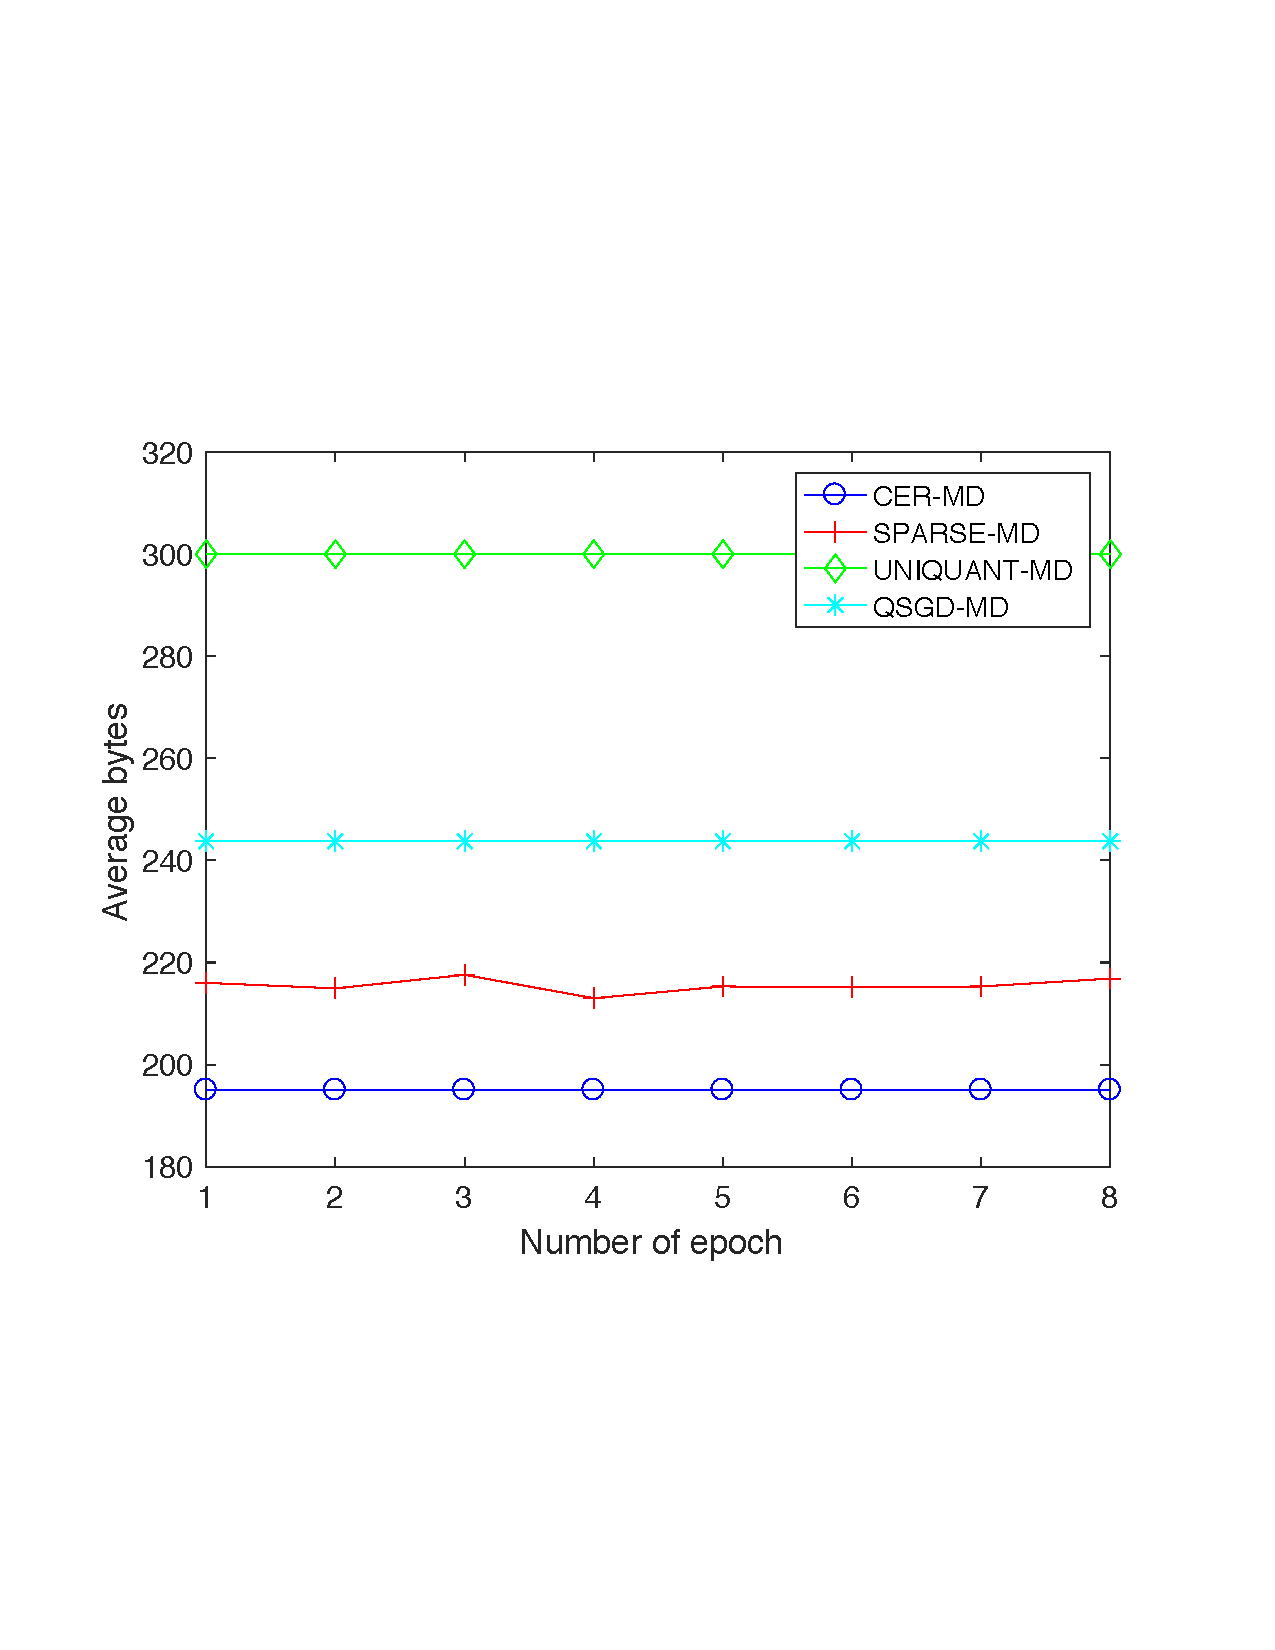
\includegraphics[width=0.32\columnwidth]{figures/figure_average_bytes_cpusmall}\label{figure_average_bytes_cpusmall}}



\caption{Comparsion of the average bytes for data transimission. Our method \textit{CER-MD} leads to the smallest amount of data transmission. }
\label{figure_average_bytes_logistic_regression}
\end{figure*}





\subsection{Numerical results} 

First, we compare the convergence performance. As illustrated in Figure \ref{figure_empirical_loss_logistic_regression}, the y-axis represents the empirical loss, and the x-axis represents the number of epoches. Here, an epoch means the entire dataset is scanned once.  Our proposed method, i.e., \textit{CER-MD} obtains the best convergence performance in the \textit{a9a} dataset, and the comparable convergence performance with other methods in the \textit{w8a} and \textit{covtype}. It shows that our method \textit{CER-MD} does not impair the convergence performance with the state-of-the-art methods. The reason is that our method jointly optimizes the empirical loss and the communication efficiency, which makes a good tradeoff between the convergence performance and the communication efficiency.

Second, we compare the workload of the data transmission. As shown in Figure \ref{figure_average_bytes_logistic_regression}, the y-axis represents the average bytes which are needed to be transmitted via network communication. The x-axis represents the number of epoches, which means how many times to scan the entire dataset. Our method \textit{CER-MD} leads to much smaller workload of data transmission. The main reason is that  \textit{CER-MD} uses the communication efficient regularizer to encourage the update of parameter to own clustering structures. The update of parameter can be encoded by using a few bits, and thus is compressed effectively. 





\begin{figure*}[!t]
\setlength{\abovecaptionskip}{0pt}
\setlength{\belowcaptionskip}{0pt}
\centering 
\subfigure[\textit{w8a, logistic regression}]{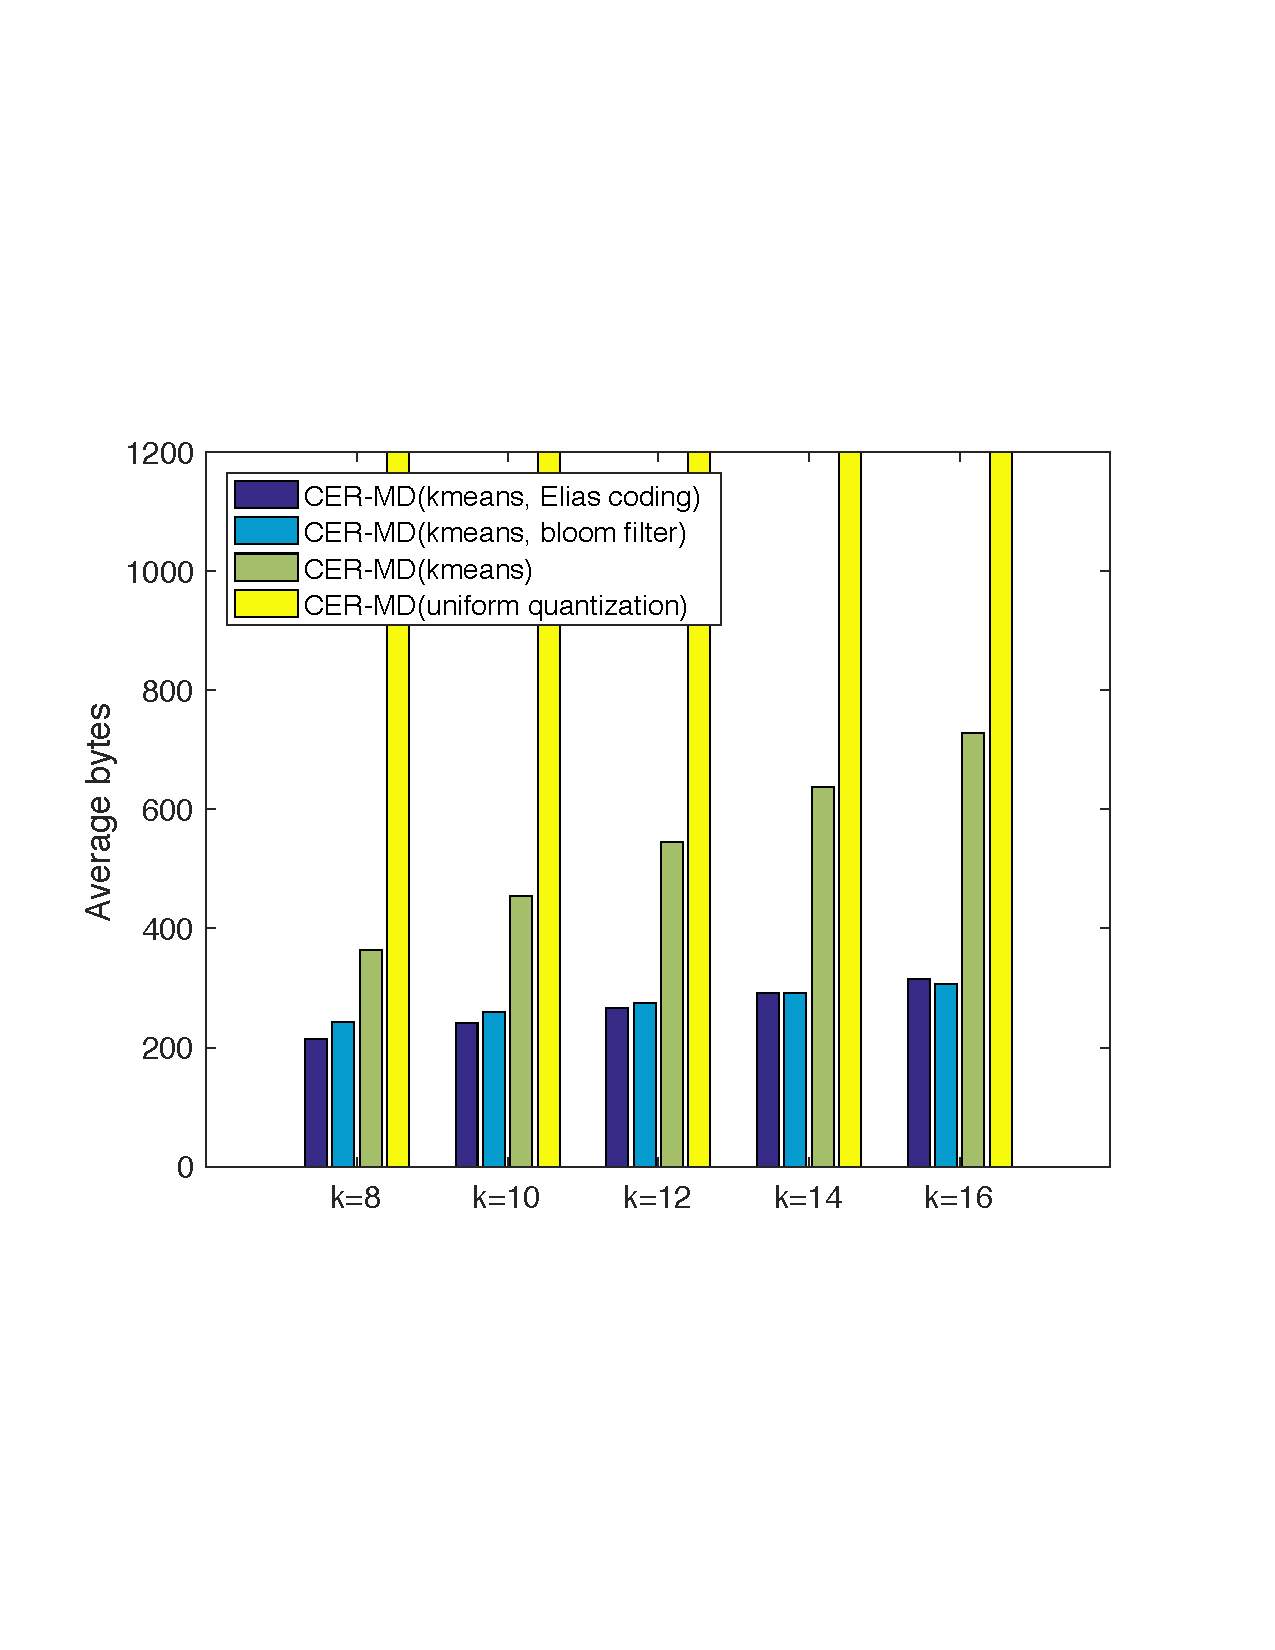
\includegraphics[width=0.335\columnwidth]{figures/figure_average_bytes_improvement_w8a}\label{figure_average_bytes_improvement_w8a}}
\subfigure[\textit{a9a, logistic regression}]{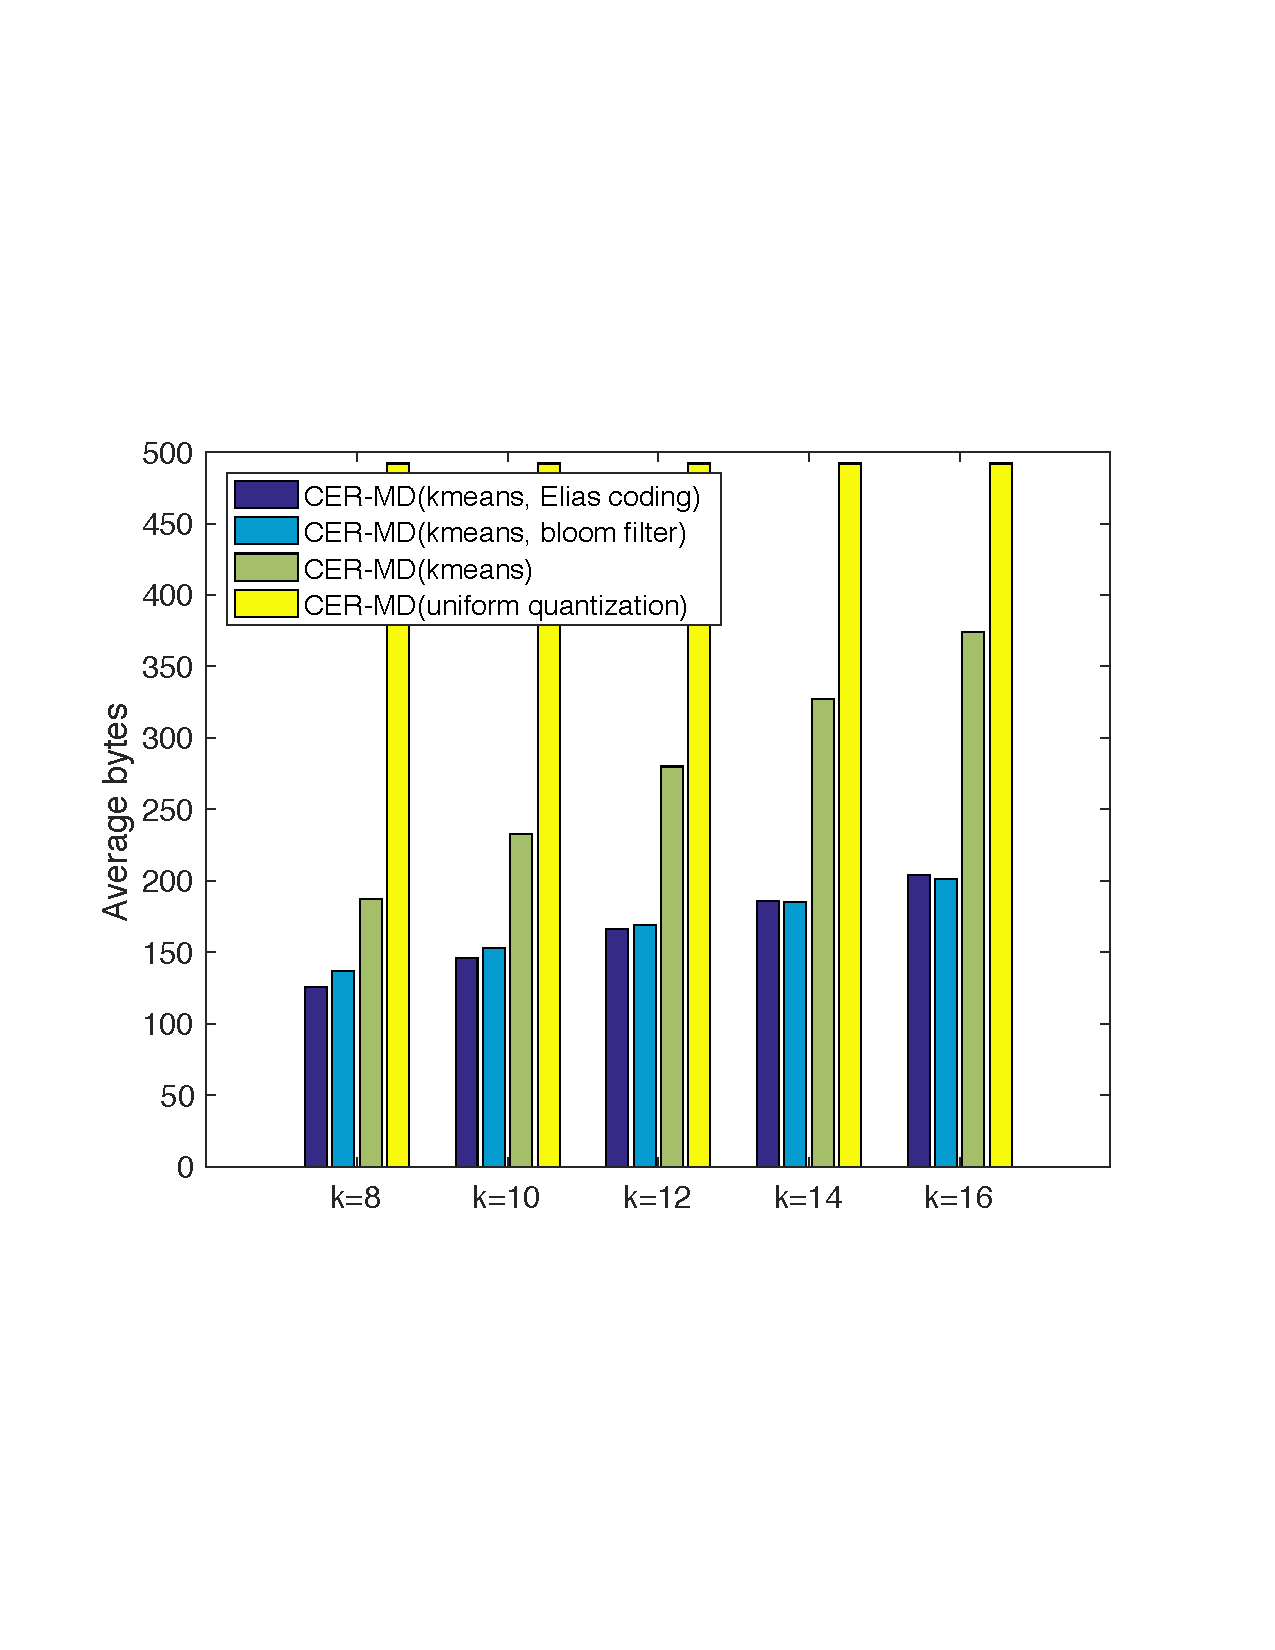
\includegraphics[width=0.325\columnwidth]{figures/figure_average_bytes_improvement_a9a}\label{figure_average_bytes_improvement_a9a}}
\subfigure[\textit{covtype, logistic regression}]{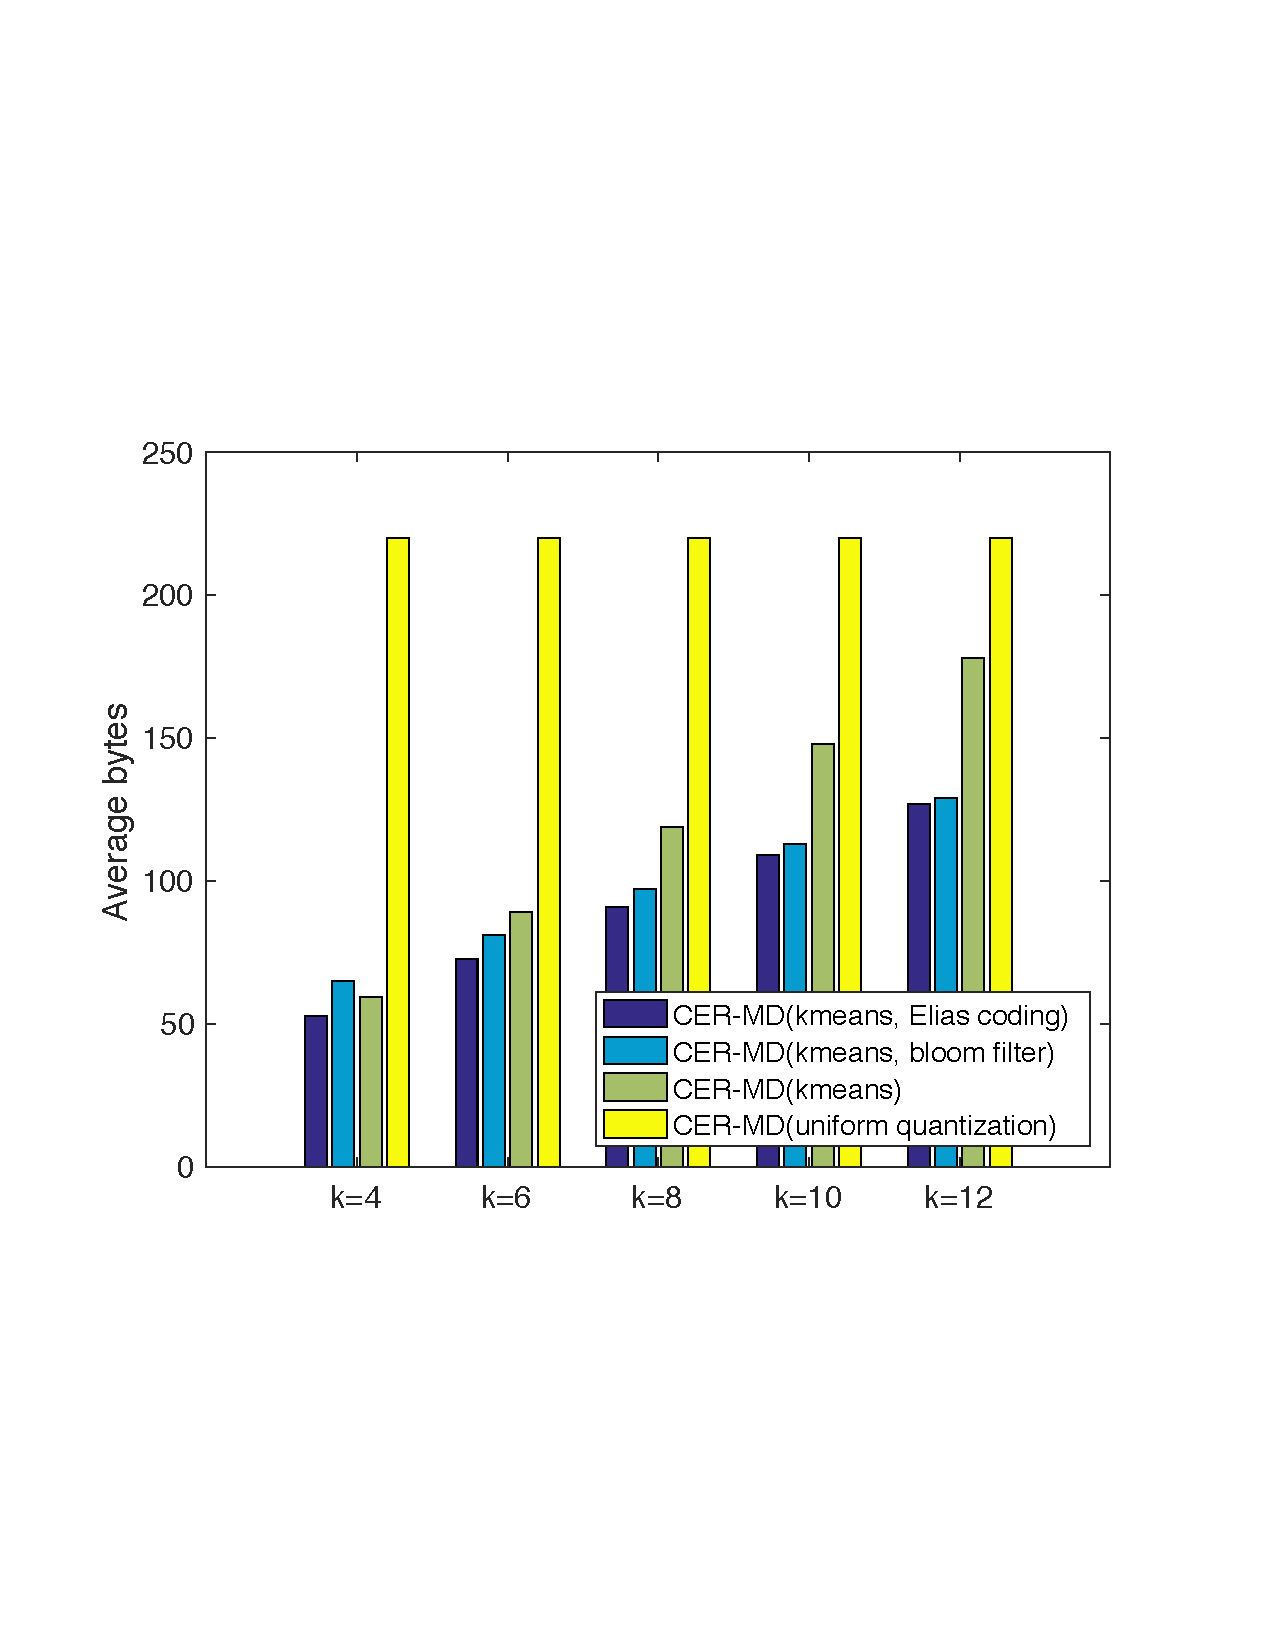
\includegraphics[width=0.325\columnwidth]{figures/figure_average_bytes_improvement_covtype}\label{figure_average_bytes_improvement_covtype}}
\subfigure[\textit{year, ridge regression}]{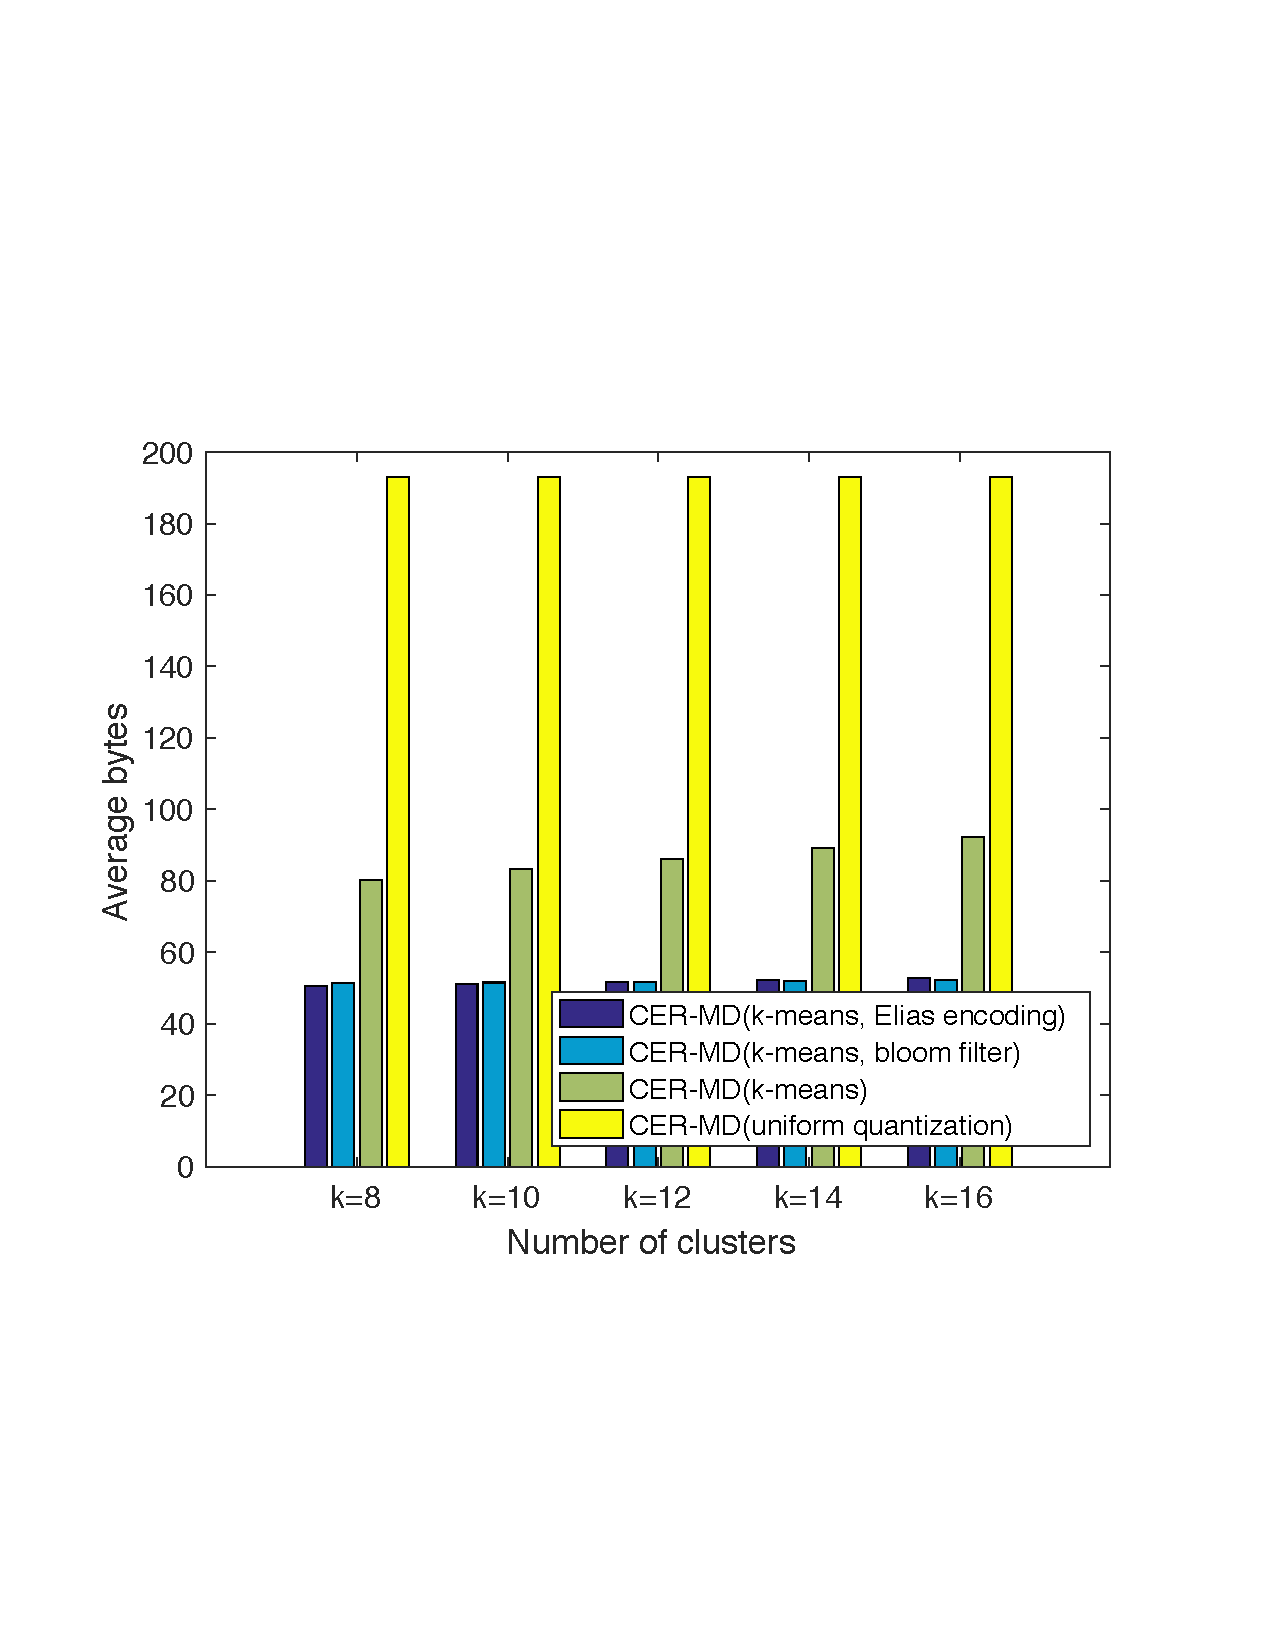
\includegraphics[width=0.335\columnwidth]{figures/figure_average_bytes_improvement_year}\label{figure_average_bytes_improvement_year}}
\subfigure[\textit{cadata, ridge regression}]{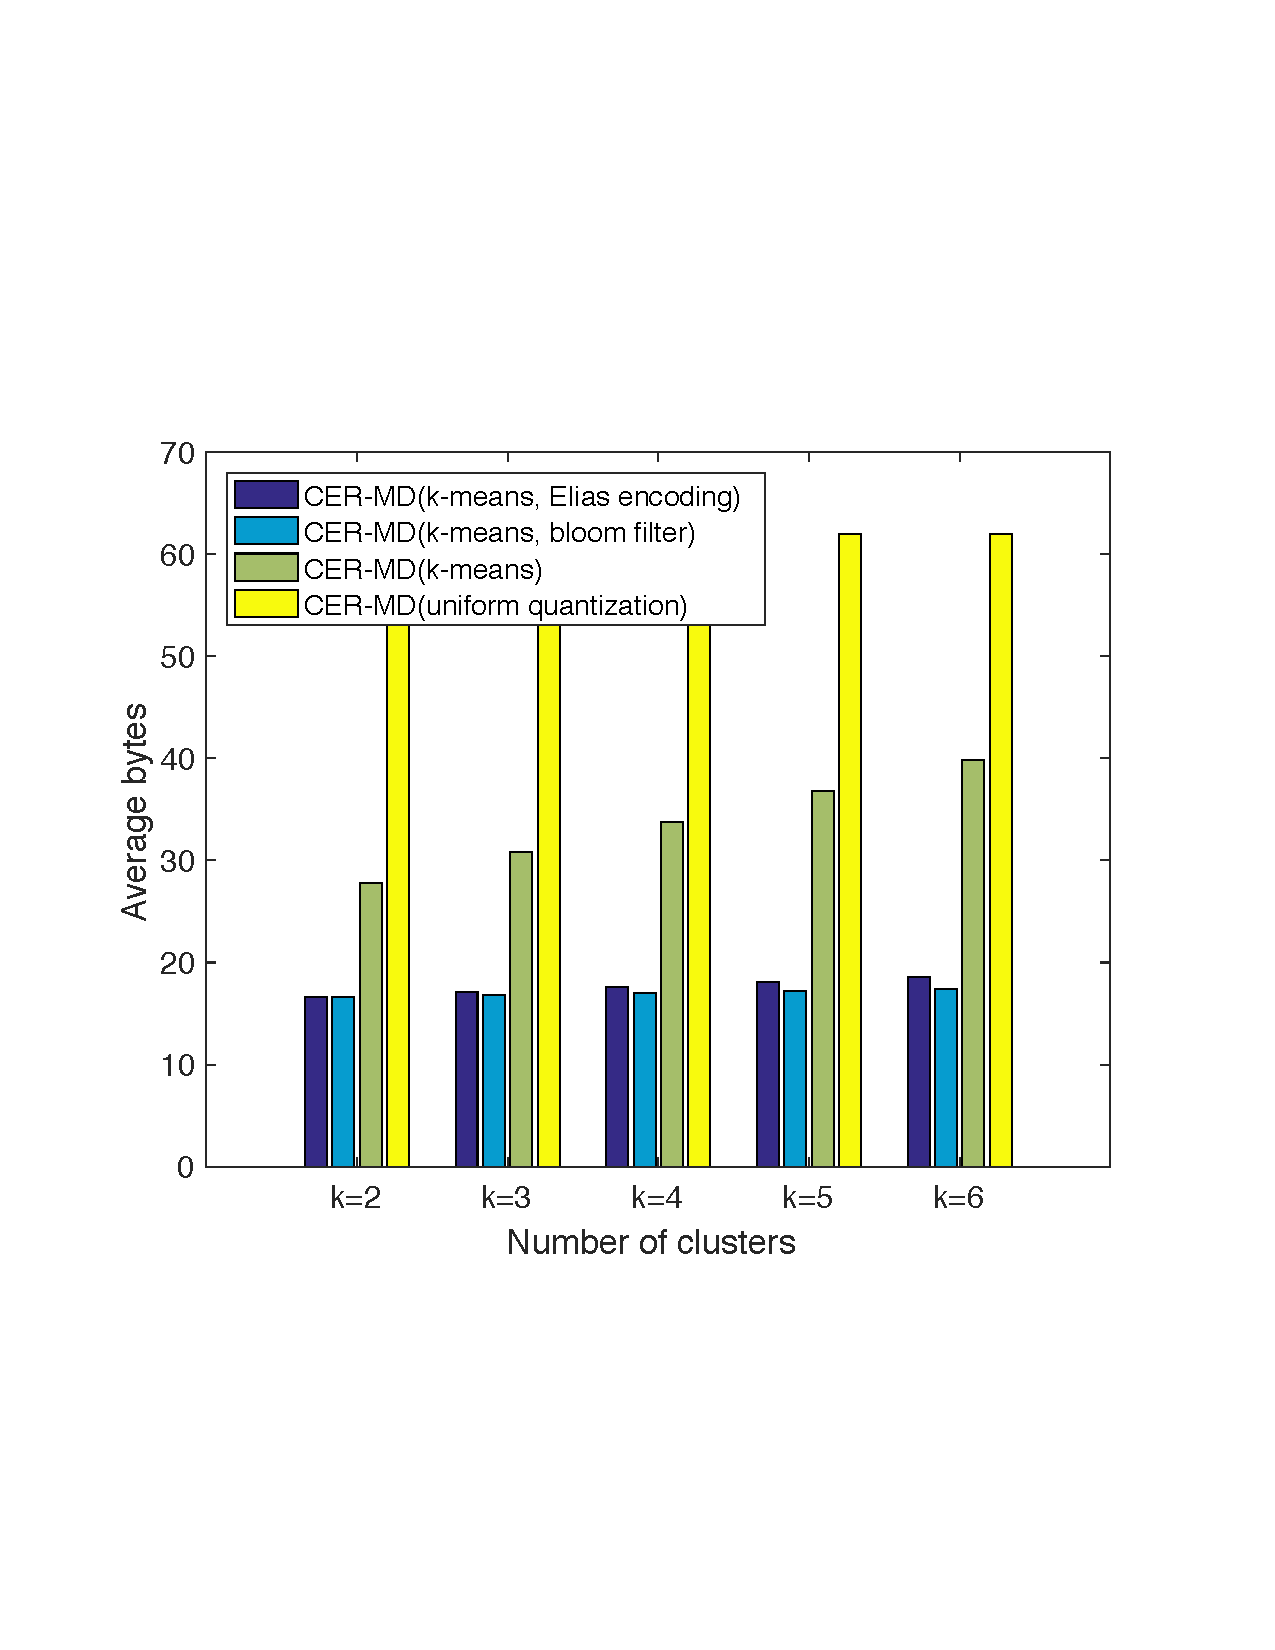
\includegraphics[width=0.325\columnwidth]{figures/figure_average_bytes_improvement_cadata}\label{figure_average_bytes_improvement_cadata}}
\subfigure[\textit{cpusmall, ridge regression}]{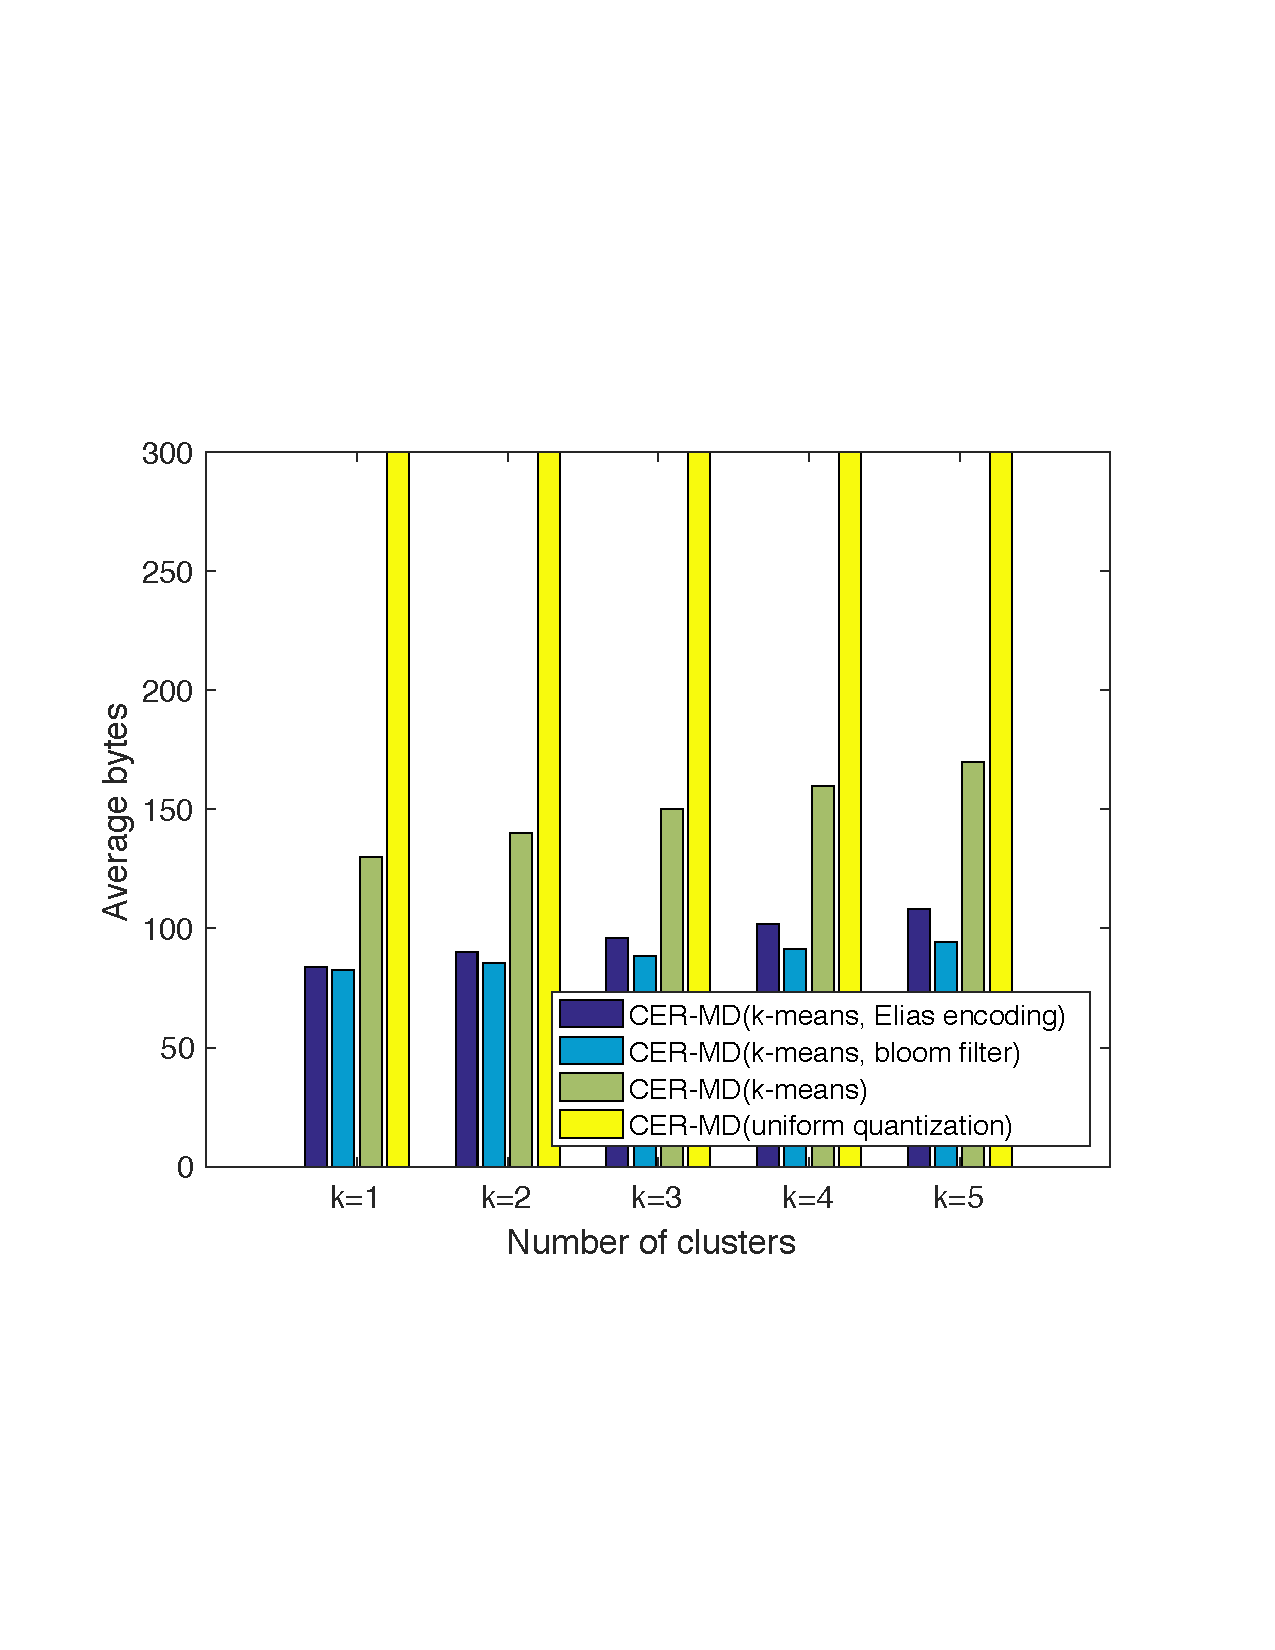
\includegraphics[width=0.325\columnwidth]{figures/figure_average_bytes_improvement_cpusmall}\label{figure_average_bytes_improvement_cpusmall}}

\caption{Comparsion of the average bytes for data transimission by varying  coding methods.}
\label{figure_average_bytes_logistic_regression_improvement}
\end{figure*}

Finally, we compare the workload of the data transmission for the proposed advanced coding methods. Those coding methods includes: \textit{kmeans clustering coding method}, \textit{uniform quantilization coding method}, \textit{kmeans clustering and Elias coding method}, and \textit{kmeans clustering and bloom filter coding method}. As illustrated in Figure \ref{figure_average_bytes_logistic_regression_improvement}, the x-axis represents the number of clusters. Since the uniform quantization method does not need to conduct clustering, the required amount of data transmission does not change with the number of clusters. We obtain some interesting observations. First, the kmeans clustering method is effective to reduce the amount of data transmission, but it leads to a large amount of data transmission with the increase of clusters. Second, with the increase of the clusters, the Elias coding method leads to more data transmission than the bloom filter method.  



\section{Conclusion}
\label{sect_conclusion}
We propose a communication efficient regularizer to jointly optimize a machine learning model and the communication efficiency. To solve it efficiently, we propose a new ADMM method. By using the linear coupling strategy, the proposed communication efficient update of the parameter obtains the sublinear convergence rate, and outperforms the state-of-the-art methods in extensive empirical studies. 


\appendix

\textbf{Proof to Lemma \ref{lemma_4}: }
\begin{proof}
Since $\y_{t+1}^{(w)} = \argmin_{\y\in\RR^d} \lrangle{\g^{(w)}_t, \y - \x_{t+1}^{(w)}} + \frac{1}{2\eta_t}\lrnorm{\Q(\y - \x_{t+1}^{(w)})}_1^2$, by setting $\eta_t = \frac{\tau\alpha_t \lrnorm{\Q}_1^2}{p-1} d^{\frac{2(p-1)}{p}}$ and denoting $C := \frac{\tau\lrnorm{\Q}_1^2}{(p-1)\sigma^2}d^{\frac{3p-2}{p}}$, we have
\begin{align}
\nonumber
& \lrangle{\g^{(w)}_t, \x_t-\v} - \frac{1}{2\eta_t}\lrnorm{\Q(\x_t-\v)}_1^2 \\ \nonumber 
\le & \lrangle{\g^{(w)}_t, \x_t-\y_{t+1}^{(w)}} - \frac{1}{2\eta_t}\lrnorm{\Q(\x_t - \y_{t+1}^{(w)})}_1^2 \\ \nonumber
\refabovecir{\le}{\textcircled{1}} & \lrangle{\g^{(w)}_t, \x_t-\y_{t+1}^{(w)}} - \frac{1}{2d\eta_t}\lrnorm{\Q(\x_t - \y_{t+1}^{(w)})}_2^2 \\ \nonumber
\refabovecir{\le}{\textcircled{1}} & \lrangle{\g^{(w)}_t, \x_t-\y_{t+1}^{(w)}} - \frac{1}{2\eta_t}\lrnorm{\Q(\x_t - \y_{t+1}^{(w)})}_2^2 \\ \nonumber
\refabovecir{\le}{\textcircled{2}} & \lrangle{\g^{(w)}_t, \x_t-\y_{t+1}^{(w)}} - \frac{\sigma^2}{2\eta_t}\lrnorm{\x_t - \y_{t+1}^{(w)}}_2^2 \\ \nonumber
\refabovecir{\le}{\textcircled{3}} & \lrangle{\g^{(w)}_t, \x_t-\y_{t+1}^{(w)}} - \frac{\sigma^2}{2d\eta_t}\lrnorm{\x_t - \y_{t+1}^{(w)}}_1^2 \\ \nonumber
= & -\lrincir{\lrangle{\nabla f(\x_t), \y_{t+1}^{(w)} - \x_t}+\frac{L_1}{2}\lrnorm{\y_{t+1}^{(w)} - \x_t}_1^2} + \lrangle{\nabla f(\x_t) - \g^{(w)}_t, \y_{t+1}^{(w)} - \x_t} \\ \nonumber 
& - \frac{1}{2}\lrincir{\frac{1}{\alpha_t C}-L_1} \lrnorm{\y_{t+1}^{(w)} - \x_t}_1^2 \\ \nonumber
\refabovecir{\le}{\textcircled{4}} & f(\x_t) - f(\y_{t+1}^{(w)})  + \frac{\tau\alpha_t\lrnorm{\Q}_1^2 d^{\frac{3p-2}{p}}\lrnorm{\nabla f(\x_{t+1}^{(w)}) - \g^{(w)}_t}_{\infty}^2}{2((p-1)\sigma^2-\tau L_1\alpha_t\lrnorm{\Q}_1^2 d^{\frac{3p-2}{p}})} \\ \nonumber %\label{equa_temp_lemma_4}
\le & f(\x_t) - f(\y_{t+1}^{(w)})  + \frac{\tau\alpha_t\lrnorm{\Q}_1^2 d^{\frac{3p-2}{p}}G}{2((p-1)\sigma^2-\tau L_1\alpha_t\lrnorm{\Q}_1^2 d^{\frac{3p-2}{p}})}.
\end{align}  $\textcircled{1}$ holds because that for any vector $\v\in\RR^d$, $\lrnorm{\v}_1\ge \lrnorm{\v}_2$. $\textcircled{2}$ holds because that for any vector $\u\in\RR^d$, $\lrnorm{\Q\u}_2 \ge \lambda_{\text{min}(\Q)}\lrnorm{\u}_2$.
$\textcircled{3}$ holds because that for any vector $\v\in\RR^d$, $\lrnorm{\v}_2 \ge \frac{1}{\sqrt{d}}\lrnorm{\v}_1$. $\textcircled{4}$ holds due to Assumption \ref{assumption_f_smooth}, and for any vectors $\u$ and $\v$,  $\lrangle{\u,\v}\le \frac{1}{2}\lrnorm{\u}_1^2 + \frac{1}{2}\lrnorm{\v}_{\infty}^2$. The proof is thus completed.

\end{proof}

\textbf{Proof to Theorem \ref{theorem}:}
\begin{proof}

Consider $\x_{t+1}^{(w)} = \tau\z_t^{(w)} + (1-\tau)\x_t$ for $0< \tau < 1$. For any vector $\u\in\RR^d$, we have 
\begin{align}
\nonumber
&f(\x_{t+1}^{(w)}) - f(\u) \le  \EE \lrangle{\g^{(w)}_t, \x_{t+1}^{(w)}-\u} \\ \nonumber
= & \lrangle{\nabla f(\x_{t+1}^{(w)}), \x_{t+1}^{(w)} - \z_t^{(w)}} + \lrangle{\nabla f(\x_{t+1}^{(w)}), \z_t^{(w)} - \u} \\ \nonumber
= & \frac{1-\tau}{\tau} \lrangle{\nabla f(\x_{t+1}^{(w)}), \x_t - \x_{t+1}^{(w)}} +  \lrangle{\nabla f(\x_{t+1}^{(w)}), \z_t^{(w)} - \u} \\ \label{equa_bound_1}
\le & \frac{1-\tau}{\tau} \lrincir{f(\x_t) - f(\x_{t+1}^{(w)})} +  \lrangle{\nabla f(\x_{t+1}^{(w)}), \z_t^{(w)} - \u}
\end{align} 



Since $\lrangle{\nabla f(\x_{t+1}^{(w)}), \z_t^{(w)} - \u} = \EE \lrangle{\g^{(w)}_t, \z_t^{(w)} - \u}$, we begin to upper bound $\lrangle{\g^{(w)}_t, \z_t^{(w)} - \u}$.
\begin{align}
\nonumber
&\lrangle{\g^{(w)}_t, \z_t^{(w)} - \u} = \lrangle{\g^{(w)}_t, \z_t^{(w)} - \z_{t+1}^{(w)}} + \lrangle{\g^{(w)}_t, \z_{t+1}^{(w)} - \u} \\ \nonumber
\refabovecir{\le}{\textcircled{1}} & \lrangle{\g^{(w)}_t, \z_t^{(w)} - \z_{t+1}^{(w)}}  + \frac{1}{\alpha_t}\lrincir{ - B_p(\z_{t+1}^{(w)}, \z_t^{(w)}) + B_p(\u, \z_t^{(w)}) - B_p(\u, \z_{t+1}^{(w)})} \\ \nonumber
\refabovecir{\le}{\textcircled{2}} & \lrangle{\g^{(w)}_t, \z_t^{(w)} - \z_{t+1}^{(w)}} - \frac{p-1}{2\alpha_t}\lrnorm{\z_{t+1}^{(w)} - \z_t^{(w)}}_p^2 + \frac{1}{\alpha_t}\lrincir{B_p(\u, \z_t^{(w)}) - B_p(\u, \z_{t+1}^{(w)})} \\ \label{equa_thm_temp1} 
\refabovecir{\le}{\textcircled{3}} & \lrangle{\g^{(w)}_t, \z_t^{(w)} - \z_{t+1}^{(w)}} - \frac{p-1}{2\alpha_t}d^{-\frac{2(p-1)}{p}}\lrnorm{\z_{t+1}^{(w)} - \z_t^{(w)}}_1^2 + \frac{1}{\alpha_t}\lrincir{ B_p(\u, \z_t^{(w)}) - B_p(\u, \z_{t+1}^{(w)})}.
\end{align}  $\textcircled{1}$ holds due to Lemma \ref{lemma_p_bregman_cosine_theorem}. $\textcircled{2}$ holds due to Lemma \ref{lemma_pnorm_strongly_convex}. $\textcircled{3}$ holds due to Lemma \ref{lemma_norms_transform}. 
%$\textcircled{5}$ holds by setting $C = \frac{1}{p-1}d^{\frac{p-1}{p}}$ with $p>1$.



Define $\v := \tau \z_{t+1}^{(w)} + (1-\tau)\y_t$. Thus, $\x_t-\v = \tau (\z_t^{(w)} - \z_{t+1}^{(w)})$. 
\begin{align}
\nonumber
& \lrangle{\g^{(w)}_t, \z_t^{(w)} - \z_{t+1}^{(w)}} - \frac{p-1}{2\alpha_t}d^{-\frac{2(p-1)}{p}}\lrnorm{\z_{t+1}^{(w)} - \z_t^{(w)}}_1^2 \\ \nonumber 
= & \frac{1}{\tau}\lrangle{\g^{(w)}_t, \x_t-\v} - \frac{p-1}{2\alpha_t \tau^2}d^{-\frac{2(p-1)}{p}}\lrnorm{\x_t-\v}_1^2 \\ \nonumber
\le &  \frac{1}{\tau}\lrincir{\lrangle{\g^{(w)}_t, \x_t-\v} - \frac{p-1}{2\tau\lrnorm{\Q}_1^2\alpha_t}d^{-\frac{2(p-1)}{p}}\lrnorm{\Q(\x_t-\v)}_1^2} \\ \label{equa_thm_temp2}
\refabovecir{\le}{\textcircled{1}}& \frac{1}{\tau} \lrincir{f(\x_{t+1}^{(w)})-f(\y_{t+1}^{(w)})} + \frac{\alpha_t\lrnorm{\Q}_1^2 d^{\frac{3p-2}{p}}G}{2((p-1)\sigma^2-\tau L_1\alpha_t\lrnorm{\Q}_1^2 d^{\frac{3p-2}{p}})}.
\end{align} $\textcircled{1}$ holds due to Lemma \ref{lemma_4}.  
Therefore, setting $\tau = \frac{1}{2}$, and substituting \eqref{equa_thm_temp2} and  \eqref{equa_thm_temp1} into \eqref{equa_bound_1}, we obtain
\begin{align}
\nonumber
& 2(f(\y_{t+1}^{(w)}) - f(\u)) \\ \nonumber
\le & f(\y_t) - f(\u)  + \frac{\alpha_t\lrnorm{\Q}_1^2 d^{\frac{3p-2}{p}}G}{2(p-1)\sigma^2- L_1\alpha_t\lrnorm{\Q}_1^2 d^{\frac{3p-2}{p}}} + \frac{1}{\alpha_t}\lrincir{ B_p(\u, \z_t^{(w)}) - B_p(\u, \z_{t+1}^{(w)})}.
\end{align} 




When $\alpha_t = \frac{(p-1)\sigma^2}{L_1\lrnorm{\Q}_1^2d^{\frac{3p-2}{p}}\sqrt{t}}$ and $\eta_t = \frac{\tau\alpha_t \lrnorm{\Q}_1^2}{p-1} d^{\frac{2(p-1)}{p}} = \frac{\sigma^2}{2L_1 \sqrt{t}}d^{-1}$, we have $2(p-1)\sigma^2- L_1\alpha_t\lrnorm{\Q}_1^2 d^{\frac{3p-2}{p}}\ge (p-1)\sigma^2$. Denote $\alpha := \frac{(p-1)\sigma^2}{L_1\lrnorm{\Q}_1^2d^{\frac{3p-2}{p}}}$, that is, $\alpha_t = \frac{\alpha}{\sqrt{t}}$. 
\begin{align}
\nonumber
2\lrincir{f(\y_{t+1}^{(w)}) - f(\u)} \le f(\y_t) - f(\u) + \frac{G}{L_1 \sqrt{t}}   + \frac{\sqrt{t}}{\alpha}\lrincir{ B_p(\u, \z_t^{(w)}) - B_p(\u, \z_{t+1}^{(w)})}.
\end{align}  Thus, we have
\begin{align}
\nonumber
& 2(f(\x_{t+1}) - f(\u)) = 2\lrincir{f\lrincir{\frac{1}{W}\sum_{w=1}^W\y_{t+1}^{(w)}} - f(\u)} \\ \nonumber
\refabovecir{\le}{\textcircled{1}} & \frac{2}{W}\sum_{w=1}^W\lrincir{f\lrincir{\y_{t+1}^{(w)}} - f(\u)} \\ \nonumber
\le & f(\y_t) - f(\u) + \frac{G}{L_1 \sqrt{t}} + \frac{\sqrt{t}}{\alpha W}\sum_{w=1}^W \lrincir{ B_p(\u, \z_t^{(w)}) - B_p(\u, \z_{t+1}^{(w)})}.
\end{align} $\textcircled{1}$ holds due to the convexity of $f(\cdot)$. Then, telescoping $t$ from $1$ to $T$, and setting $\u = \y_{\ast}$, we have
\begin{align}
\nonumber
&\sum_{t=1}^{T}(f(\y_{t}) - f(\y_{\ast})) \\ \nonumber
\le & 2(f(\y_1) - f(\y_{T+1})) + \frac{G}{L_1}\sum_{t=1}^{T}\frac{1}{\sqrt{t}} + \frac{2}{\alpha W} \sum_{w=1}^W\lrincir{B_p(\y_{\ast},\z_1^{(w)}) + \sum_{t=2}^{T}(\sqrt{t+1}-\sqrt{t}) B_p(\y_{\ast},\z_t^{(w)})} \\ \nonumber
\refabovecir{\le}{\textcircled{1}} & 2(f(\y_1) - f(\y_{T+1})) + \frac{2G\sqrt{T}}{L_1} + \frac{2}{\alpha}\lrincir{R +  R\sqrt{T+1}}. 
\end{align} $\textcircled{1}$ holds due to $\sum_{t=1}^{T}\frac{1}{\sqrt{t}} \le 2\sqrt{T}$ and $\sum_{t=2}^{T}(\sqrt{t+1}-\sqrt{t}) \le \sqrt{T+1}$.   Finally, we obtain
\begin{align}
\nonumber
& f\lrincir{\frac{1}{T}\sum_{t=1}^T\y_t} - f(\y_{\ast})  
\le \frac{1}{T}\sum_{t=1}^T\lrincir{f(\y_t) - f(\y_{\ast})} \\ \nonumber
\le  &  \frac{2(f(\y_1) - f(\y_{T+1}))}{T} + \frac{2G}{L_1\sqrt{T}} + \frac{2L_1\lrnorm{\Q}_1^2d^{\frac{3p-2}{p}}}{(p-1)\sigma^2}\lrincir{\frac{R}{T} +  \frac{R\sqrt{T+1}}{T}}.
\end{align}
\end{proof}



\section{Acknowledgments}
This work was supported by the National Key R \& D Program of China 2018YFB1003203 and the National Natural Science Foundation of China (Grant No. 61672528, 61773392, and 61671463). 



\bibliographystyle{ACM-Reference-Format}
\bibliography{reference}


\end{document}
\endinput
%%
%% End of file `sample-acmsmall.tex'.
